% abcplus_en.tex  -*- LaTeX -*-
%
% By Guido Gonzato, PhD <guido.gonzato (at) gmail.com>
%
% Last updated: March 30, 2012
%
% This document converts to PDF only!

\documentclass[a4paper,fullpage,12pt]{book}

% ----- PACKAGES

\usepackage{color}
% \usepackage[italian]{babel} % <<<=== your language here!
%
% TRANSLATORS PLEASE READ THIS:
%
% Babel modifies the behaviour of some characters. If you experience
% odd problems, please refer to Babel's documentation.
% For example, the Italian translation needs the following:
%
% \shorthandoff{"} to turn off the shorthand character "
% \char94 instead of `\^' or \textasciicircum{} to insert `^'
%
\usepackage[pdftex]{graphicx}
\usepackage{pslatex}  % PostScript fonts
\usepackage{alltt}    % verbatim with \ support
\usepackage{booktabs} % better looking tables
\usepackage{upquote}  % to fix the ' character in pdf output
\usepackage{textcomp} % for \textquotesingle
\usepackage{framed}   % framed & shaded regions
\usepackage{lettrine} % dropped capitals
\usepackage{fancybox} % for \Ovalbox
\usepackage{fancyvrb} % for fancypage
\usepackage[margin=2.6cm]{geometry}
\usepackage{setspace} 
\usepackage{supertabular} % table spanning over 2 pages
\usepackage{boxedminipage}
\usepackage{marvosym}
\usepackage{wasysym}  % for \twonotes and other symbols
\usepackage[colorlinks,linkcolor=darkred,%
urlcolor=blue,filecolor=blue,breaklinks=true]{hyperref}
\urlstyle{same}

% ----- format.tex

% ----- DEBUG
% \overfullrule=5pt
% \widowpenalty=10000
% \clubpenalty=10000

\frenchspacing % we're in Europe after all - \@ not necessary
\setlength{\parindent}{0pt}
\setlength{\parskip}{3pt}
% \setlength{\parskip}{1ex plus 0.5ex minus 0.2ex}
% \graphicspath{{./images/}}

\definecolor{defaultshadecolor}{rgb}{0.85,0.85,1}
\definecolor{shadecolor}{rgb}{0.85,0.85,1}
\definecolor{gray}{rgb}{0.7,0.7,0.7}
\definecolor{charcolor}{rgb}{1,0.85,0.85}
\definecolor{lightred}{rgb}{1,0.7,0.7}
\definecolor{darkblue}{rgb}{0,0,0.5}
\definecolor{darkred}{rgb}{0.75,0,0}

% ----- DEFINITIONS

\newcommand{\version}{March 2012} % VERSION

\newcommand{\abcmdev}{7.0.3}
\newcommand{\abcmstable}{6.6.8}
\newcommand{\abcmoldstable}{5.9.25}
\newcommand{\abcmidi}{2012\_03\_27}
\newcommand{\ABCPLUS}{\textsc{Abc Plus}}
\newcommand{\ABC}{\textsc{Abc}}
\newcommand{\abcm}{\texttt{abcm\-2ps}}
\newcommand{\abctab}{\texttt{abc\-tab\-2ps}}
\newcommand{\abcpp}{\texttt{abc\-pp}}
\newcommand{\abcmid}{\texttt{abc\-2mi\-di}}
\newcommand{\abcMID}{\texttt{abc\-MI\-DI}}
\newcommand{\abcprt}{\texttt{abc\-2prt}}
\newcommand{\jedabc}{\textsc{Jed\-Abc}}
\newcommand{\abcexplorer}{ABC\-ex\-plo\-rer}
\newcommand{\runabc}{\texttt{run\-abc.\-tcl}}
\newcommand{\easyabc}{Easy\-ABC}
\newcommand{\ps}{Post\-Script}
\newcommand{\bl}{\textbackslash}
\newcommand{\qs}{\textquotesingle}
% \newcommand{\devel}{\textcolor{darkred}{\Industry}}

% ----- NEW COMMANDS AND ENVIRONMENTS

\newcommand{\entry}[2]
{\textsf{#1/#2}}

\newcommand{\app}[1]
{\texttt{#1}}

\newcommand{\menu}[1]
{\textsf{#1}}

\newcommand{\file}[1]
{\texttt{#1}}

\newcommand{\field}[1]
{\texttt{#1}}

\newcommand{\cmd}[1]
{\texttt{#1}}

\newcommand{\icmd}[1]
{\textit{\texttt{#1}\/}}

\newcommand{\metacmd}[1]
{\texttt{\%\%#1}}

\newcommand{\parm}[1]
{\textit{$\langle$#1$\rangle$}}

\newcommand{\optparm}[1]
{\textit{[#1]}}

\newcommand{\car}[1]
{\colorbox{charcolor}{\rule{0pt}{1ex}\texttt{#1}}}

\newcommand{\notes}[1]
{\texttt{#1}}

\newcommand{\graph}[1]
{\textsc{#1}}

\newcommand{\noteseparator}
{\begin{center}
\twonotes~\twonotes~\twonotes~\twonotes~\twonotes~\twonotes~\twonotes\
\end{center}}

\newenvironment{margins}[2]
{ % begin def
\begin{list}{}
{
\setlength{\leftmargin}{#1}
\setlength{\rightmargin}{#2}
} \item
} % end def
{\end{list}}

\newenvironment{abcsource}
{ % beg def
  \begin{snugshade}
    \begin{alltt}
}
{ % end def
    \end{alltt}
  \end{snugshade}
}

\newenvironment{bytheway}
{ % beg def
  \definecolor{shadecolor}{rgb}{0.9,0.9,0.9}
  \begin{flushright}
    \begin{minipage}{0.92\linewidth}
      \begin{snugshade}
  }      
{ % end def
      \end{snugshade}
    \end{minipage}
  \end{flushright}
}

\newenvironment{note}
{ % beg def
  \definecolor{shadecolor}{rgb}{0.9,0.9,0.9}
  \begin{flushright}
    \begin{minipage}{0.92\linewidth}
      \begin{snugshade}
        {\large \Writinghand}~~\textbf{Note}
}
{ % end def
      \end{snugshade}
    \end{minipage}
  \end{flushright}
}

\newenvironment{warn}
{ % beg def
  \definecolor{shadecolor}{rgb}{1,0.85,0.85}
  \begin{flushright}
    \begin{minipage}{0.92\linewidth}
      \begin{snugshade}
         {\large \Pointinghand}~~\textbf{Warning}
}
{ % end def
  \end{snugshade}
    \end{minipage}
  \end{flushright}
}

\newenvironment{vimp}
{ % beg def
  \definecolor{shadecolor}{rgb}{1,0.85,0.85}  
  \begin{flushright}
    \begin{minipage}{0.92\linewidth}
      \begin{snugshade}
        \textcolor{red}%
	{\large \Stopsign}~~\textbf{Very important!}
}
{ % end def
      \end{snugshade}
    \end{minipage}
  \end{flushright}
}

\newcommand{\score}[1]
{
\begin{margins}{-1cm}{-1cm}
  \includegraphics[width=\linewidth]{#1.pdf}
\end{margins}
}

\newcommand{\scoreshort}[1]
{
\includegraphics{#1.pdf}
}

\newcommand{\scorepage}[1]
{
\includegraphics[width=\linewidth]{#1.pdf}
}

% ----- End of file format.tex
 % ----- low-level formatting stuff

% ----- Let's start -----

\pagestyle{headings}

\begin{document}

\frontmatter

\setcounter{tocdepth}{3}
\thispagestyle{empty}

% ----- Title page

\begin{titlepage}

  \setcounter{page}{0}

  \pagecolor{shadecolor}
  \thisfancypage{
  \Ovalbox}{}
  \centering

  {
    \null % placeholder
    \vspace{0.5cm}

    \resizebox{!}{0.6cm}{\textit{Guido Gonzato}}

    \vspace{6cm}

    \resizebox{!}{1.15cm}{Making Music with}

    \bigskip

    \resizebox{!}{1.35cm}{\ABCPLUS{}}

    \vspace{4cm}

    \setlength{\fboxsep}{1cm}
    {\includegraphics[width=.65\textwidth]{titlepage.pdf}}

    \vfill

    \resizebox{!}{0.55cm}{\textit{A guide to the notation and
    its applications}}
  
    \vspace{1cm}

  }

\end{titlepage}

% ----- Copyright (copyleft actually)

% \pagestyle{plain}
\thispagestyle{empty}
\pagecolor{white}
\null
\vfill

\textit{Making Music with \ABCPLUS}

Copyleft \textcopyright{} Guido Gonzato, PhD, 2003--2012

Latest update: \today

Typeset with \LaTeX, with the help of the
\href{http://www.jedsoft.org/jed/}{Jed editor} and
\href{http://www.ctan.org/pkg/latex4jed}{
{\LaTeX\kern-.2em\raise.3ex\hbox{\sc 4}\kern-.15em\textsc{Jed.}}
}

This manual is released under the terms of the GNU Free Documentation
License,

\url{http://www.gnu.org/licenses/fdl.html}

\bigskip

The latest version of this manual is available at:

\url{http://abcplus.sourceforge.net/#ABCGuide}

\newpage

% ----- Dedication

\thispagestyle{empty}
\null
\vfill

{\large
\begin{flushright}
\begin{itshape}
To Annarosa,

Bruno,

Lorenzo

\Heart

\end{itshape}
\end{flushright}
}

\vfill
\null
\newpage

% ----- Table of contents

\thispagestyle{empty} % for empty page before TOC
\setcounter{page}{4}
\pagestyle{plain}

%  no page numbers
% \fancypagestyle{plain}
% {
%   \fancyhead{}
%   \fancyfoot{}
% }

\tableofcontents
\listoftables
\listoffigures

% -----

\chapter{About This Book}

\lettrine{T}{his} manual explains how to make beautiful sheet music
and MIDI files using a computer, some free software, and the
\ABCPLUS{} music notation.

It's aimed at musicians with some computer expertise who don't want to
spend a lot of money on commercial music software. Both folk and
classical musicians may benefit from this guide, not to mention music
teachers!

This manual comes in printed and electronic versions; the latter is
accompanied by a few audio files. Just like the software that is used
to make the music, this manual is free and can be freely copied and
shared.

I hope you will find my work useful and enjoyable.

Cheers,

\hspace{2cm}Guido Gonzato \texttt{=8-)}

% -----

\mainmatter

\pagenumbering{arabic}
\pagestyle{headings}

\chapter{Music on the Computer with \ABCPLUS}

\section{Introduction}

\lettrine{I}{f} you are a musician and if you can use a computer, you
are lucky. First of all, because you are a musician; secondly, because
the computer is a precious tool for writing music. Lots of programs
are available, even for free.

Most music notation programs have a visual approach: one or more
staves are displayed on the screen, and the user drags and drops notes
and symbols using the mouse. An alternative approach is writing music
using a \emph{text-based notation}. This is a non-visual mode that
represents notes and other symbols using characters. A specialised
program then translates the notation into printable sheet music in
some electronic format (e.g.\ in PDF) and/or into a MIDI file.

Visual programs are easier for beginners and are probably more
intuitive, but text-based notations make for faster transcription and
have other advantages.

Many text-based notations have been invented. \ABC{}, introduced by
Chris Walshaw in 1991, is one of the best: being simple, easy to learn
yet very powerful, it has gained widespread popularity. Thousands of
tunes written in \ABC{} are available on the Internet: in fact,
this notation is the de facto standard among folk musicians. The
\ABC{} home page is \url{http://abcnotation.com}.

\ABC{} was later expanded to provide multiple voices
(po\-ly\-pho\-ny), page layout details, and MIDI commands. This was
called \ABC{} 2.1: its formal description is available at
\url{http://abcnotation.com/wiki/abc:standard:v2.1}.

A few programs implement most \ABC{} 2.1 features and provide some
extensions. In this guide, this extended notation will be informally
called \ABCPLUS. The purpose of this guide is to introduce the reader to
\ABCPLUS{} and the most important features of its related programs.
Ideally, people who could benefit from this manual are:

\begin{itemize}
  
  \item folk musicians who would like to learn as little \ABC{} as
  necessary to understand the files they find on the net. These people
  can skip the part about harmony, and probably do not need to study
  this guide thoroughly;
  
  \item classical musicians who would like to use \ABCPLUS{} for
  typesetting their scores.
  
\end{itemize}

In both cases, if you wish to print sheet music for your choir or
band, or make a song book, or perhaps just teach music, you have found
the right tool. And it's also free!

The \ABCPLUS{} home page is \url{http://abcplus.sourceforge.net}.

\paragraph{A Few Words About ``Standards''.}

While \ABC{} is formally defined, the status of \ABCPLUS{} is a bit
fuzzy. It has no official definition, and it can be described as
``whatever feature and/or extension to \ABC{} 2.* is implemented by
the best software available''. In other words, \ABC{} 2.* is a
theoretical standard, while \ABCPLUS{} is what you can do with
available programs. It should be emphasised that \ABCPLUS{} is fully
upwards compatible with \ABC; in the future, these two ``releases'' of
the same music notation language might even merge.

For the sake of simplicity, in the following I shall simply write
``\ABC{}'' instead of ``\ABCPLUS{}''.


% -----

\subsection{Requirements}

I assume that you have a PC with Windows, Mac OS X, GNU/Linux or other
Unix variants, and that you are reasonably familiar with computers.
Expertise in the Windows or Unix command line interface is not
required. It is required, however, that you can read music: the treble
clef and two octaves starting at middle C should suffice.

% -----

\subsection{Software}

The state of the art of \ABC{} is currently represented by two great
little programs: the \abcm{} typesetter, and the MIDI creator \abcmid.
Both are free software released under the GNU GPL license.

\abcm{} reads \ABC{} files and converts them to \ps. This is a format
related to PDF, and it can be viewed and printed with another free
program: Ghostscript. This application converts \ps{} files into
several formats, Acrobat PDF being the most important.

% TO DO: cite Sumatra, ps_view

The author of \abcm, an organist and programmer called Jean-Fran\c
cois Moine, releases ``stable'' and ``development'' versions of his
program. The latter has many enhancements, but it may be buggy. As of
this writing,\footnote{\today.} the stable release is \abcmstable, the
previous stable release is \abcmoldstable, the development release is
\abcmdev. This guide will only describe features of the former stable
release \abcmoldstable; the new release introduces several changes
(most notably, SVG output, UTF--8 support, and transposition) which
will be described in future versions of this guide. 

\abcmid{} converts \ABC{} files to MIDI. It is part of the \abcMID{}
package, which include other utility applications. Its usage will be
described in Part~\ref{sec:sound} (page~\pageref{sec:sound}) of this
guide.

Since \ABC{} files are plain text files, an essential tool for writing
them is a good text editor. Countless free editors exist, some of
which have facilities for editing \ABC{} files. In general, any
application that can be used to write text can also be used to write
\ABC{} files.

% \begin{note}

%   There also exist graphical applications that save music in \ABC{}
%   format, some of which are very nice. These programs make it
%   unnecessary to learn the \ABCPLUS{} notation using this manual---at
%   least the basics. Therefore, I will not describe them here.

% \end{note}

\abcm{} and \abcmid{} are \emph{command-line driven} programs: in
short, you cannot start them double-clicking on their icons. To use
these programs, you have to open a command shell (Windows Command
Prompt or Unix terminal) and type commands. Geeky stuff.

Scared off? Don't worry: the command line can be avoided. There exist
programs that gather all relevant pieces of software in a single
integrated environment:

\begin{itemize}

  \item \abcexplorer{} (Figure~\ref{fig:abcexplorer}), a Windows
  application;
  
  \item \easyabc, multiplatform;
  
  \item \jedabc{} (Figure~\ref{fig:jedabc}), primarily designed for
  GNU/Linux but also available on Windows;
  
  \item \runabc, multiplatform;
  
  \item The Folkinfo Abc Converter (Figure~\ref{fig:folkinfo}): a web
  interface to \abcm{} and \abcMID. Highly recommended.
  
\end{itemize}

I feel that none of these programs are ``perfect''; however, I would
suggest that Windows users adopt \abcexplorer, while GNU/Linux and Mac
OS X users may prefer \jedabc{} or \runabc{} to other
general-purpose editors like \app{vim} or \app{gedit}. The Folkinfo
converter is probably the easiest solution, as you don't have to
install anything.

Many more applications are available and are listed on the \ABC{}
home page.

\begin{figure}[htbp]
\centering
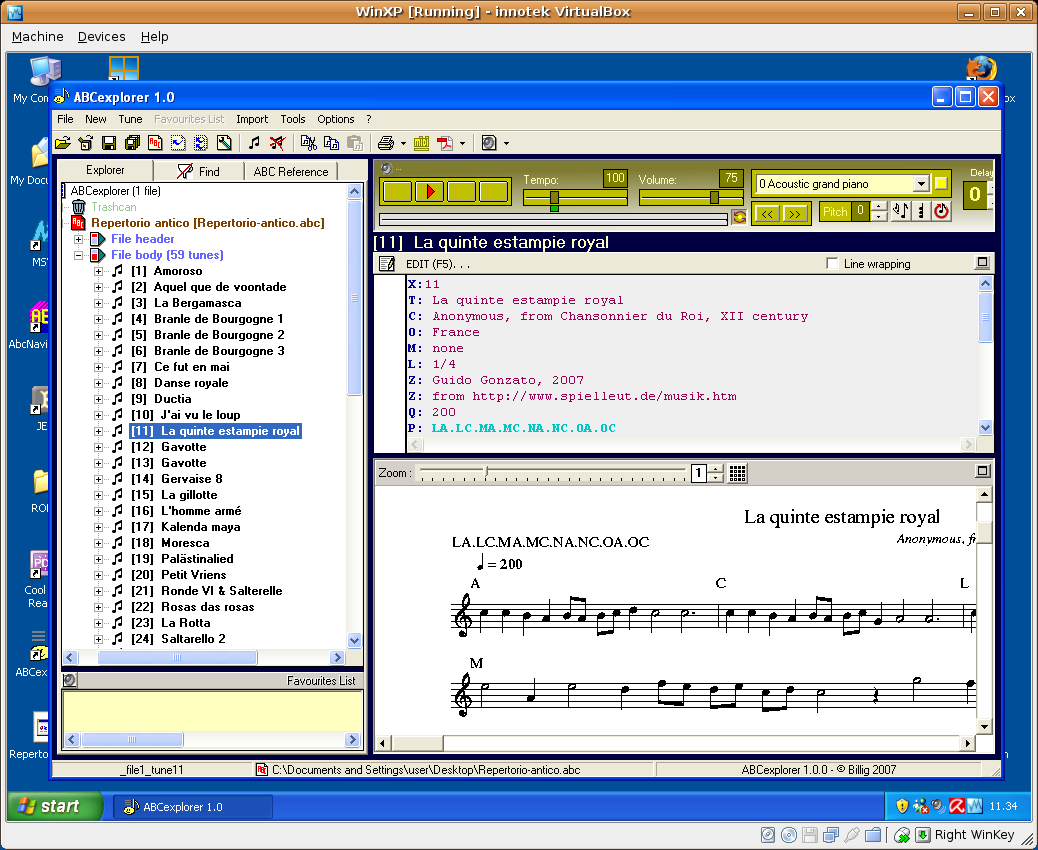
\includegraphics[width=0.8 \linewidth]{screenshot-win.png}
\caption{Managing a tune collection with \abcexplorer.}
\label{fig:abcexplorer}
\end{figure}

\begin{figure}[htbp]
\centering
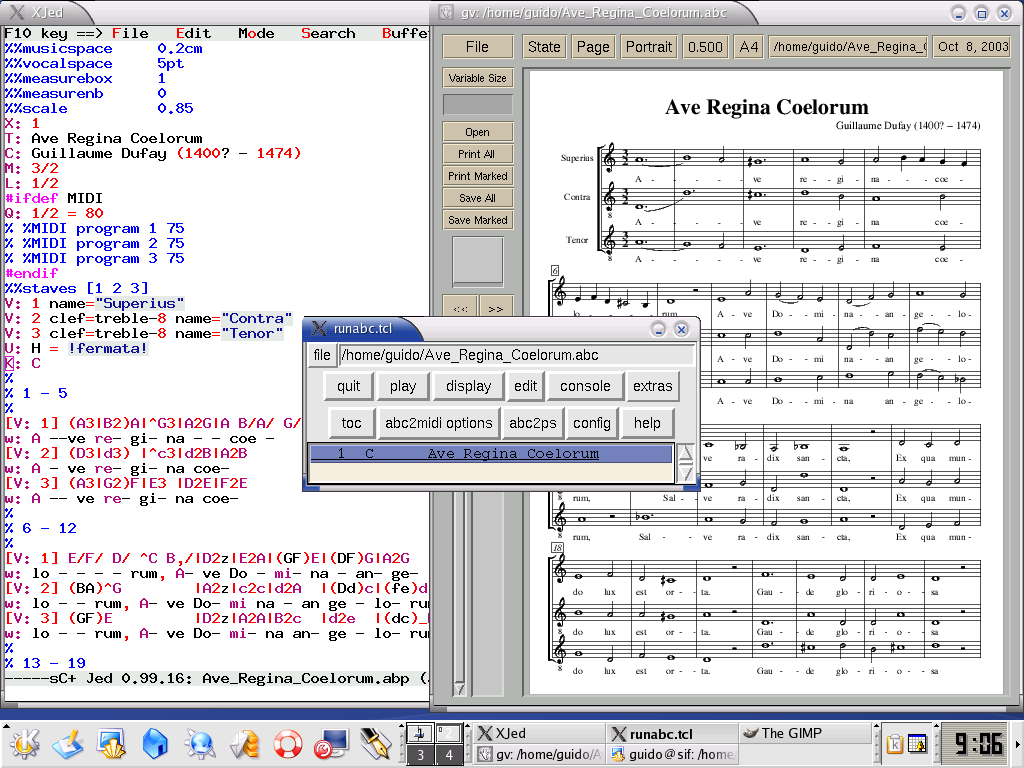
\includegraphics[width=0.8 \linewidth]{screenshot-linux.png}
\caption{Writing a tune with \jedabc{} and \runabc.}
\label{fig:jedabc}
\end{figure}

\begin{figure}[htbp]
\centering
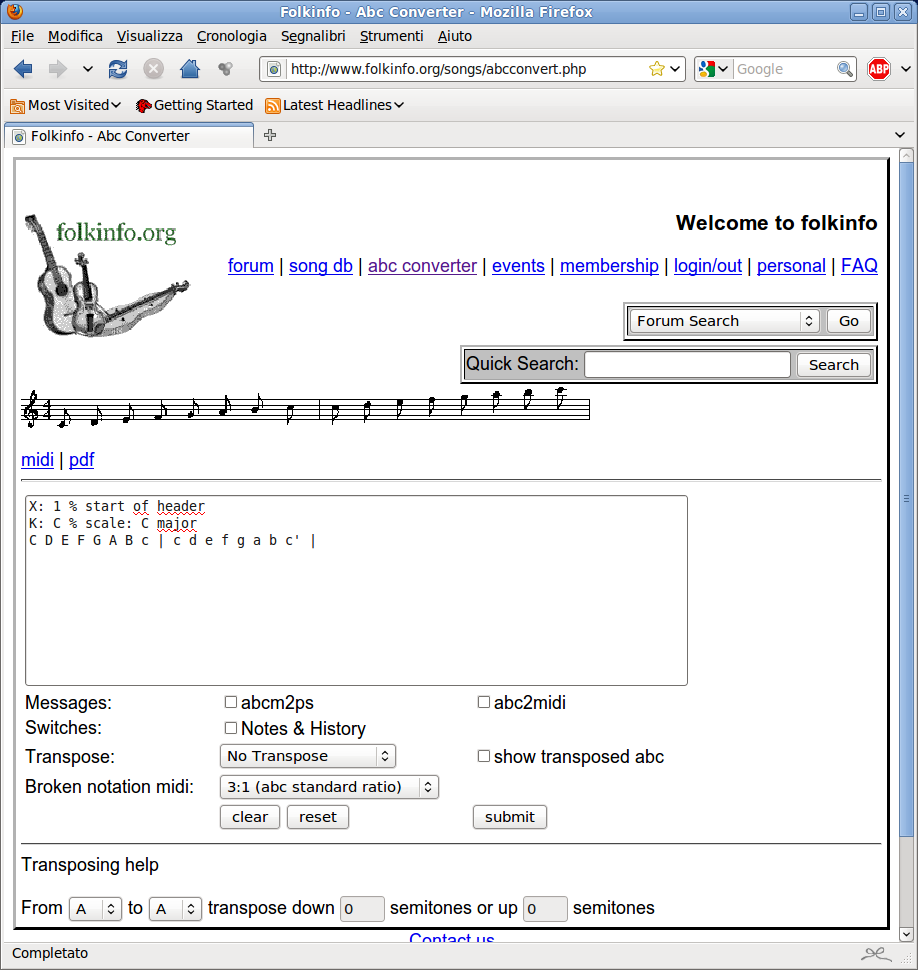
\includegraphics[width=0.8 \linewidth]{screenshot-folkinfo.png}
\caption{Writing a tune with the Folkinfo abc converter.}
\label{fig:folkinfo}
\end{figure}

% -----

\subsection{Why \ABC{}?}

I know from experience that graphical programs (nearly all are
commercial software) are considered easier to use than non-graphical
ones.\footnote{erroneously, but only expert users realize it.} So, why
should one learn \ABC?

Well, compared to graphical programs \ABC{} has many advantages:

\begin{description}
  
  \item [smart:] \ABC{} allows for small and readable files, ea\-sy
  se\-ar\-ching and indexing of tunebooks, easy creation of music
  archives, etc;
  
  \item [text only:] the importance of this feature can't be
  overemphasised. Being simple text, \ABC{} music can be read and
  written by any computer system on Earth; can be used by visually
  impaired people, texted by phone, scribbled down on beermats,
  {\ldots}
  
  \item [scalability:] with \ABC{} you can create scores from very
  simple to highly sophisticated;
  
  \item [ease of use:] \ABC{} is easy to learn, and after a little
  practice it becomes very intuitive;
  
  \item [quality:] using \abcm, \ABC{} produces publication quality
  sheet music;
  
  \item [price:] while commercial software is often expensive, nearly
  all programs for making \ABC{} music are free, and can be freely
  copied and shared with your friends or students;
  
  \item [low resources:] \ABC{} programs are very compact and can run
  on old computers, or even handhelds or smartphones;
  
  \item [portability:] music is created as \ps{} or PDF and
  MIDI files instead of proprietary file formats. This way, you can
  share your music with everybody, not only people who have the
  software to produce it;
  
  \item [flexibility:] inserting music written in \ABC{} in web pages
  or word processor files is very simple;
  
  \item [speed:] writing music in \ABC{} is \emph{much} faster than
  using any graphical program;
  
  \item [learning value:] if you teach music, \ABC{} in an invaluable
  tool that facilitates the learning of music theory;
  
  \item [fun:] in my humble opinion, writing music in \ABC{} is more
  fun!
  
\end{description}

Needless to say, there are disadvantages as well:

\begin{description}
  
  \item [learning curve:] while a graphical program may allow you to
  get started right away (at least in theory), \ABC{} requires that
  you take your time and study the syntax before you can get started;
  
  \item [file conversion:] if your work environment forces you to use a
  specific commercial program, you may find it difficult or impossible
  to convert existing music files to \ABC{} and vice versa;
  
  \item [limitations:] \ABC{} can't do everything. Currently, it can't
  deal with some types of music, such as Gregorian chant and
  non-European music.
  
\end{description}

To overcome the first hurdle, this guide is hopefully a good start;
but I also recommend that you look at some scores to see real-life
examples of \ABC{} in action. The \ABC{} home page has many links to
\ABC{} collections; on the \ABCPLUS{} page you will find more complex
choral scores.

% In my opinion, there is little reason to use other music programs
% (often an illegal copy), given the many advantages of switching to
% \ABCPLUS{}. Read this manual and see what \ABCPLUS{} can do for you.
% You will not regret it!

% -----

\section{Getting Started}

In order to write music with \ABC, you follow these steps:

\begin{enumerate}
  
  \item using an editor, write the tune using the \ABC{} syntax;
  
  \item convert the tune using \abcm{}, creating a \ps{} file;
  
  \item view the \ps{} file with Ghostscript or other viewer;
  
  \item convert the \ps{} file into PDF format;
  
  \item create a MIDI file with \abcmid;
  
  \item finally, if the music you wrote is free from copyright, publish
  it for others to enjoy!
  
\end{enumerate}

% -----

\subsection{Installing the Programs}

Relevant web pages:

\begin{itemize}
  
  \item the \abcm{} typesetter:\\
  \url{http://moinejf.free.fr}\\
  \url{http://abcplus.sourceforge.net/#abcm2ps}

  \item \abcmid:\\
  \url{http://ifdo.pugmarks.com/~seymour/runabc/top.html}\\
  \url{http://abcplus.sourceforge.net/#abcMIDI}

  \item Ghostscript and GSview:\\
  \url{http://pages.cs.wisc.edu/~ghost}
  
  A rather old but convenient version is Ghostscript 5.50, packaged
  with GSview 2.7. Unlike newer releases of GSview, this release has
  no nag screen, and is especially suitable for use with \jedabc. Get
  the installer \file{gsv27550.exe} from:
  
  \url{ftp://mirror.cs.wisc.edu/pub/mirrors/ghost/aladdin/gs550/}
  
  European mirror:\\
  \url{ftp://mirror.switch.ch/mirror/ghost/aladdin/gs550/}
  
  However, if you wish to convert the scores to PDF files you will
  need the latest release of Ghostscript from this directory:\\
  \url{http://mirror.cs.wisc.edu/pub/mirrors/ghost/GPL/}\\ and the
  latest GSview from:\\
  \url{http://mirror.cs.wisc.edu/pub/mirrors/ghost/ghostgum/}
  
  \item \abcexplorer:\\
  \url{http://abc.stalikez.info/abcex.php}

  \item \easyabc:\\
  \url{http://www.nilsliberg.se/ksp/easyabc/}

  \item \jedabc{}:\\
  \url{http://abcplus.sourceforge.net/#JedABC}
  
  \item \app{runabc}:\\
  \url{http://ifdo.pugmarks.com/~seymour/runabc/runabc.html}
  
  \item The Folkinfo converter:\\
  \url{http://www.folkinfo.org/songs/abcconvert.php}
  
\end{itemize}

Ready-to-run packages for Windows, GNU/Linux, and Mac OS X are
available from the \ABCPLUS{} web site. Besides, all GNU/Linux
distributions include Ghostscript and the \app{gv}, \app{evince}, and
\app{okular} viewers.

I assume that GNU/Linux and Mac OS X users will be able to install the
programs. On Windows, the easiest and highly recommended solution is
installing \abcexplorer, which includes all relevant programs;
alternatively, download \abcm{} and \abcmid{}, extract the \file{.exe}
files from the archives, then copy them to \path{C:\WINDOWS}.
Ghostscript and GSview are installed like any standard Windows
applications.

% -----

\subsection{\ABC{} in a Nutshell}
\label{sec:nutshell}

\ABC{} music is written in text files with extension \file{.abc} or
\file{.abp}. The extension is not obligatory, but highly recommended.

\ABC{} uses the characters you find on standard computer keyboards to
represent notes and symbols:

\begin{itemize}
  
  \item characters like \car{A B C a b c z} represent notes and rests;
  
  \item accidentals, ties, slurs etc.\ are written with characters like
  \car{= \_ - ( )} and so on;
  
  \item expression symbols are notated with words like \cmd{!fff!},
  \cmd{!fermata!}, \cmd{!tenuto!}, {\ldots}
  
  \item the metre, clef, title, and other tune properties are written
  in words called \emph{fields}, like \field{M:}, \field{K:},
  \field{T:};
  
  \item low-level details (that is, formatting parameters or MIDI
  commands) are written using \emph{commands} like \metacmd{titlefont}
  or \metacmd{MIDI program 19}.
  
\end{itemize}

In short: all musical features are written with sequences of
characters.

A tune, which is written in an \emph{\ABC{} file}, consists of two
parts: a \emph{header} and a \emph{body}. The header contains
information about the tune such as the title, author, key, etc.; these
pieces of information are written in fields. The body of the tune
contains the music.

An \ABC{} file may contain several tunes, separated by one or more
blank lines. Each tune has its own header and body. Some fields can
also appear in the body. The file containing \ABC{} music is also
called the \emph{source} of the tunes.

Strictly speaking, commands for low-level details are not part of the
notation. In fact, \ABC{} was designed for a high-level description of
tunes, with no special instructions for typesetting or sound output.
That said, \ABCPLUS{} provides commands for specifying such details;
these will be examined in Section~\ref{sec:format}.

If you don't have a US keyboard, some important characters may be
missing. To obtain these characters under Windows, turn the numeric
keypad on, keep the \fbox{Alt} key pressed and type some digits:

\begin{itemize}
  
  \item \cmd{Alt-126} to get the \emph{tilde} \car{\textasciitilde};
  
  \item \cmd{Alt-009} to get a \emph{tab character};
  
  \item \cmd{Alt-096} to get an \emph{inverted accent} \car{`}.
  
  \item \cmd{Alt-123} to get an \emph{open curly bracket} \car{\{};
  
  \item \cmd{Alt-125} to get a \emph{closed curly bracket} \car{\}};
  
  \item \cmd{Alt-091} to get an \emph{open square bracket} \car{[};
  
  \item \cmd{Alt-092} to get a \emph{closed square bracket} \car{]}.
  
\end{itemize}

% -----

\subsection{Our First Score}
\label{sec:first}

When the programs are installed, we are ready to write our first
score. As our first example, we shall write the C major scale and
study the source carefully.

In the following, I'll describe the very basic commands: the
command-line interface, plus an editor. You will see that it's not
that difficult after all. Anyhow, remember that you can use the
Folkinfo converter.

There's a very important detail to stress beforehand. Whenever you
write an \ABC{} file, you'll have to choose a file name. Any file name
will do, \emph{but}:

\begin{vimp}

  \emph{do not use file names containing spaces!}

\end{vimp}

That is: instead of, say, \file{My music file.abc}, you must write
\file{My-\-music-\-file\-.abc} or \file{My\-Music\-File\-.abc}. It's
very important, because \abcm{} cannot easily use filenames containing
spaces. Besides, file names containing spaces are not web-friendly
either.

Ok? Good. Let's proceed. Commands you must enter are printed in
\textbf{boldface}.

% -----

\paragraph{Windows.}

Start the \cmd{cmd} program. (Windows XP: from
\entry{Start}{Run{\ldots}}, insert \cmd{cmd}, then click on ``Ok''.
Windows 7: start the menu then insert \cmd{cmd} in ``Search Programs
and Files''.)

A black window will pop up showing a line that reads something like:

\begin{verbatim}
C:\Users\Guido>_
\end{verbatim}

The first time, and only the first time you use the command prompt,
type this command:

\begin{alltt}
C:\bl{}Users\bl{}Guido>\textbf{md abcmusic}
\end{alltt}

and press the \fbox{Enter} key. This command creates a directory
(folder), called \cmd{abcmusic}, where we will save our \ABC{} files.
Now, let's enter (double click) the folder:

\begin{alltt}
C:\bl{}Users\bl{}Guido>\textbf{cd abcmusic}
C:\bl{}Users\bl{}Guido\bl{}abcmusic>_
\end{alltt}

Note that the command prompt changed to confirm that you've moved to
that folder. Move to the \file{abcmusic} folder before writing tunes.

Let's now run the \cmd{notepad} editor. In our example, we'll use the
file name \file{scale1.abc}.

\begin{alltt}
C:\bl{}Users\bl{}Guido\bl{}abcmusic>\textbf{notepad scale1.abc}
\end{alltt}

Clic on ``Yes'' to create a new file, then copy this source 
\emph{verbatim}:

\begin{abcsource}
X: 1 % start of header
K: C % scale: C major
C D E F G A B c | c d e f g a b c' |
\end{abcsource}

Save it, then switch back to the command prompt.

We are ready to make the \ps{} output using \abcm:

\begin{alltt}
C:\bl{}Users\bl{}Guido\bl{}abcmusic>\textbf{abcm2ps -c -O= scale1.abc}
abcm2ps-5.9.25 (November 2, 2011)
File scale1.abc
Output written on scale1.ps (1 page, 1 title, 17899 bytes)
C:\bl{}Users\bl{}Guido\bl{}abcmusic>_
\end{alltt}

To display the \ps{} file, launch GSview and open the \file{scale1.ps}
file that you'll find in \path{C:\Documents and
Settings\user\abcmusic}. The score will look like this:

\medskip

\score{scale1}

\medskip

To convert the score into PDF, select \entry{File}{Convert{\ldots}} in
GSview, set \cmd{pdfwrite} as output type, and choose a dpi
resolution; I suggest 600 dpi.

Now, let us make a mistake on purpose: insert the \car{\#} character
instead of the first bar \car{\textbar}. Save and try to convert; you
will get this error message:

\begin{alltt}
C:\bl{}Users\bl{}user\bl{}abcmusic>\textbf{abcm2ps -c -O= scale1.abc}
abcm2ps-5.9.25 (November 2, 2011)
File scale1.abc
Error in line 3.16: Bad character
   3 C D E F G A B c # c d e f g a b c' |
                     ^
Output written on scale1.ps (1 page, 1 title, 17877 bytes)
C:\bl{}Users\bl{}user\bl{}abcmusic>_
\end{alltt}

Fix the error in the source, save it and convert it again.


% -----

\paragraph{GNU/Linux and Mac OS X.}

Open a terminal window (Ubuntu: Applications/Accessories; Mac OS X:
Applications/Utilities). The first time, and only the first time you
use the command prompt, type this command:

\begin{alltt}
$ \textbf{mkdir abcmusic}
\end{alltt}

and press the \fbox{Enter} key. This command creates a directory (folder),
called \cmd{abcmusic}, where we will save our \ABC{} files. Now, let's
enter (double click) the folder:

\begin{alltt}
~$ \textbf{cd abcmusic}
~/abcmusic$ _
\end{alltt}

The command prompt should change to confirm that you've moved to that
folder. Move to the \file{abcmusic} folder before writing tunes.

Now let's start an editor. In GNU/Linux systems, it's likely to be
\app{gedit} or \app{kate} (if it's not, please find out). In Mac OS X,
it's simply called \app{edit}. The file name is \file{scale1.abc}.

\begin{alltt}
~/abcmusic$ \textbf{gedit scale1.abc &}
\end{alltt}

Don't forget the ampersand \car{\&} at the end of the line. Copy this
source \emph{verbatim}:

\begin{abcsource}
X: 1 % start of header
K: C % scale: C major
C D E F G A B c | c d e f g a b c' |
\end{abcsource}

Save it, then switch back to the command prompt. We are ready to make
the \ps{} output using \abcm:

\begin{alltt}
~/abcmusic$ \textbf{abcm2ps -c -O= scale1.abc}
abcm2ps-5.9.25 (November 2, 2011)
File scale1.abc
Output written on scale1.ps (1 page, 1 title, 17899 bytes)
~/abcmusic$ _
\end{alltt}

To display the \ps{} output, GNU/Linux users should use the \app{gv}
or \cmd{evince} or \cmd{okular} viewer. Mac OS X has a Preview utility
that will automatically open \file{scale1.ps} and convert it into PDF
format.

\begin{alltt}
~/abcmusic$ \textbf{evince scale1.ps &}
\end{alltt}

The score will look like this:

\medskip

\score{scale1}

\medskip

Finally, to convert the file into PDF type this command:

\begin{alltt}
~/abcmusic$ \textbf{ps2pdf scale1.ps}
~/abcmusic$ _
\end{alltt}

The file \file{scale1.pdf} will be silently created.

\begin{warn}

  Probably, an environment variable needs to be set in order to get A4
  paper format from \cmd{ps2pdf}. Insert this line in
  \file{/etc/profile}:
  
  \medskip
  
  \cmd{export GS\_OPTIONS="-sPAPERSIZE=a4"}
  
  \medskip
  
  If you use the \app{gv} viewer, remember to set the correct paper
  format, otherwise the page margins will be displayed incorrectly.
  
\end{warn}

Now, let us make a mistake on purpose: insert the \car{\#} character
instead of the first bar \car{\textbar}. Save and try to convert; you
will get this error message:

\begin{alltt}
~/abcmusic$ \textbf{abcm2ps -c -O= scale1.abc}
abcm2ps-5.9.25 (November 2, 2011)
File scale1.abc
Error in line 3.16: Bad character
   3 C D E F G A B c # c d e f g a b c' |
                     ^
Output written on scale1.ps (1 page, 1 title, 17877 bytes)
~/abcmusic$ _
\end{alltt}

Fix the error in the source, save it and convert it again.

% ----

Let us now examine what we wrote in the source. It starts with two
header fields: \field{X:}, index, and \field{K:}, key; both
upper-case. These are the only obligatory fields. \field{X:} is always
followed by a number, which is used to identify the tunes written in a
file. The \car{\%} character begins a comment; everything that follows
\car{\%} till the end of the line is ignored.

Fields may contain spaces. \field{X:1} and \field{X: 1} are
equivalent.

The \field{K:} field specifies the tune key; \car{C} stands for ``C
major''. In some countries, notes are written as ``do (ut) re mi fa
sol la si (ti)''; if you live in such a country, you may want to
consult Table~\ref{tab:note} that compares notes written in English
and in Italian notation. I call it ``Italian notation'' since it was
introduced by medieval Italian composer Guido d'Arezzo.

\begin{table}[h]
\begin{center}
\begin{tabular}{ll}
\toprule % \hline
\textbf{Italian note} & \textbf{English note} \\
\midrule % \hline
Do & C \\
Re & D \\
Mi & E \\
Fa & F \\
Sol & G\\
La & A \\
Si & B\\
\bottomrule % \hline
\end{tabular}
\caption{Comparison between note names in different notations.}
\label{tab:note}
\end{center}
\end{table}

The \field{X:} field must be \emph{the first} in the header, while the
\field{K:} field must be \emph{the last}. Other fields may be inserted
in any order between \field{X:} and \field{K:}.

The next line in the source starts the body of the tune, containing
the notes. Upper-case letters correspond to the central octave, while
lower-case letters one octave higher. The \car{\textbar} character
inserts a measure bar, which can be entered at any position. That is,
you may write measures of variable length, more than or less than the
value specified by the metre.

The last \car{c} is followed by an apostrophe, which denotes an octave
higher. Note that \abcm{}, by default, automatically set the metre as
four quarters, and the note length as eighths.

It wasn't difficult, was it? We are now ready to study all the details
that will enable us to typeset beautiful scores.

\begin{note}

  If you use ``do re mi{\ldots}'', the main hurdle is getting used to
  ``C D E{\ldots}'' A trick I used was memorizing the notes as
  ``doC'', ``reD'', ``miE'', ``faF'', ``solG'', ``laA'', ``siB'' and
  the reverse.
  
\end{note}

Homework time. Try and write some \ABC{} files as an exercise. Type
random notes if you wish, but get used to writing, saving, converting,
and viewing tunes. I suggest that you do your exercises at the end of
each of the following sections.

\noteseparator

% -----

\chapter{Melody}

\section{Notes and Symbols}
\label{sec:note}

\lettrine{T}{his} part of the manual deals with basic characteristics
of notes: pitch, length, accidentals, dots, ties, slurs, tuplets,
chords, grace notes, and expression symbols.

\begin{note}

  In some of the following examples, formatting parameters were
  removed from the sources for clarity.

\end{note}

% -----

\subsection{Pitch: \icmd{A-G a-g ,'}}
\label{sec:pitch}

The following source (\file{scale2.abc}) shows how to obtain notes
under and above the staff, i.e. notes that sit on ledger lines; the
scale is C major. Instead of just writing \field{K:C} as in the
previous example, we'll add a small bit of code which will be further
explained in Section~\ref{sec:clefs}. \field{K:C treble}, besides
specifying C major, forces the treble clef. In this example it must be
specified because there are several notes much below the staff, and
\abcm{} would set the bass clef by default. Convert the source without
\cmd{-c}:

\begin{abcsource}
X: 1
K: C treble
% C major, four octaves:
C, D, E, F, G, A, B, C | C D E F G A B c |
c d e f g a b c' | c' e' g' c'' |
\end{abcsource}

\score{scale2}

The rule is: if a note is followed by one or more commas, it goes down
one or more octaves; if it is followed by one or more apostrophes, it
goes up one or more octaves.\footnote{Experts will notice some
resemblance to the Helmholtz pitch notation, shifted two octaves.} 

Note another important detail: we wrote two lines of \ABC{} notes,
which produced two lines of music. This is one of the basic rules of
the \ABC{} notation: \emph{a new line in the source starts a new
line in the score.} Exceptions will be examined in
Section~\ref{sec:battute}.

In the above example, note spacing is too wide; a single line would
probably look better. We can instruct \abcm{} to ignore line breaks
and try and format the measures optimally. This is done with \cmd{-c}
in the command line.

We'll now reformat the file using \cmd{-c}:

\begin{verbatim}
$ abcm2ps -O= -c scale2.abc
\end{verbatim}

% $

\score{scale3}

The bass clef is automatically set when we start a piece of music with
low notes (\car{F,} and below). The treble clef is then set by \abcm{}
for higher notes:

\begin{abcsource}
X: 1
M: 4/4
L: 1/8
K: C
%
C,, D,, E,, F,, G,, A,, B,, C,|C, D, E, F, G, A, B, C|
C D E F G A B c|c d e f g a b c'|
\end{abcsource}

\score{scale4}

% -----

\subsection{Note Length: \icmd{L:}}
\label{sec:length}

Unless otherwise indicated, the \emph{note length} is automatically
set in accordance to the tune metre.

The rule is: if the value of the metre is greater than or equal to
0.75, the default note length will be one eighth; if it is less than
0.75, one sixteenth. For example, when the metre is 4/4 the value is 1
(4 divided by 4 is 1), so the note length will be one eighth; if the
metre is 3/4 = 0.75, again one eighth; if the metre is 2/4 = 0.5, the
note length will be one sixteenth. By default, the metre is 4/4 and
the note length is one eighth.

The \field{L:} field is used to modify the default note length,
specifying a value as in \field{L:1/4}. (To change the metre, the
\field{M:} field is used; see Section~\ref{sec:metre}.)

To double, triple etc.\ the length of a note, you write the number 2,
3, etc.\ immediately after. To divide the value of a note by 2, 4
etc., you write \car{/2}, \car{/4}, \car{/8}{\ldots} or, equivalently,
\car{/}, \car{//}, \car{///}{\ldots} Spaces between the note and the
digit or the slash are not allowed. Let us see an example:

\begin{abcsource}
X: 1
L: 1/4
K: C
C16|C8|C4|D2 D2|E0 E E F/ F/ F/ F/|
G3 G// G/4 G/8 G/8 G/16 G/16 G/16 G/32 G/32 |
\end{abcsource}

\score{length}

Note that \abcm{} supports notes as short as 1/128 and longer than a
whole note! The first note in the example is called a \emph{longa},
and its length is four whole notes. The second note is a
\emph{brevis}, two whole notes. The spacing between notes is
proportional to their length. (We shall see in
Section~\ref{sec:format} how to make the spacing of notes constant
instead of proportional.) Another weird note is the first \car{E} in
measure 5: the trailing \car{0} denotes a stemless quarter
note.\footnote{these peculiar note lengths are sometimes found in
early music.}

Spaces between notes and measure bars can be freely inserted when the
notes are longer than one eighth, and are used to improve the
readability of the source. But \emph{spaces between notes whose length
is equal or lesser than one eighth are not optional}. If these notes
are not separated by spaces, they will be grouped under a beam:

\begin{abcsource}
X: 1
K: C
M: 4/4
% 
C D E F CDEF | C D E F C/D/E/F/G/A/B/c/ |
c/B/A/G/ F/E/D/C/ C4 |
\end{abcsource}

\score{groups}

% -----

\subsection{Rests and Spacing: \icmd{z Z x y}}
\label{sec:rests}

Rests are indicated by the character \car{z} (lowercase zed). The same
rules for note length apply to rests too, which can also be longer
than a whole and as short as 1/128.

To notate multi-measure rests, you use \car{Z} (uppercase zed)
followed by the number of measures you want to skip:

\begin{abcsource}
X: 1
L: 1/4
K: C
Z12|z16|z8|z4|C2 z2|C z C z|
C z/ z/ C z//z//z///z///z///z////z////|
\end{abcsource}

\score{rests}

The characters \car{x} and \car{y} denote, respectively,
\emph{invisible rests} and additional spacing:

\begin{abcsource}
X: 1
L: 1/4
K: C
C D E/E/E/E/ F/F/F/F/|C D E/E/E/yyE/ F/yF/yF/yF/ yyyy|xxxG|
\end{abcsource}

\score{rests2}

\car{y} can be followed by a width in \emph{points}; default is 20
points. This unit of measurement is widely used in typography; a
``point'' (\ps{} point) is $\approx$ 0.353mm.

Invisible rests are often used for transcribing piano music; examples
will be shown in Section~\ref{sec:staves}.

% -----

\subsection{Accidentals: \icmd{\textasciicircum \_ =}}

Sharp $\sharp$ is denoted by a \car{\textasciicircum} before the note,
flat $\flat$ by \car{\_} (underscore), and natural $\natural$ by
\car{=}. Spaces between the accidental and the note are not allowed.
This is the chromatic scale:

\begin{abcsource}
X: 1
L: 1/4
K: C
C ^C D ^D | E F ^F G | ^G A ^A B | c^c=cz |
c B _B A | _A G _G F | E _E D _D | C_C=Cz |
\end{abcsource}

\score{accid}

Double accidentals are indicated doubling the special character:
double sharp $\sharp\sharp$ by \car{\char94\char94} and double flat
$\flat\flat$ by \car{\_\_}.

Quarter tone accidentals are also available. That is, 1/4 and 3/4
sharps and flats can be obtained adding \car{/} after \car{\char94} or
\car{\_}, while 3/4 are obtained adding \cmd{3/2}:

\begin{abcsource}
X: 1
M: 4/4
L: 1/8
K: C
G ^/G ^G ^3/2G A4|A _/A _A _3/2A G4|G3 ^G A4|A3 _A G4|]
\end{abcsource}

\score{microtonal}

\begin{note}
  
  Unlike normal accidentals, microtonal accidentals don't propagate
  across a whole measure. This is an important thing to remember 
  when you make a MIDI file, to avoid unexpected results.
 
\end{note}

% -----

\subsection{Dotted Notes: \icmd{\textless{} \textgreater{}}}

Notes followed by a dot are printed in two ways. First, by specifying
the right length:

\begin{abcsource}
X: 1
L: 1/4
K: C
C3D|E3/2 F//G// A B| c3/2 B//A// G>F|E D C z|
\end{abcsource}

\score{dotted2}

When a note is dotted and the following is halved or vice versa, we
are talking of \emph{broken rhythm}. It is obtained using the
characters \car{\textgreater} or \car{\textless} between two notes.

When you use \car{\textgreater}, the first note is dotted (that is,
its duration increases by half) and the following note is halved. The
opposite with \car{\textless}. To indicate a note followed by two or
three dots, use \car{\textgreater\textgreater} or
\car{\textgreater\textgreater\textgreater}.

\begin{abcsource}
X: 1
L: 1/4
K: C
CEGc|C > E G >> c|C < E G < c|C/>E/ C/ > E/ C/<E/ C/ < E/|
\end{abcsource}

\score{dotted}

\begin{note}
  
  Dotted notes are rendered by \abcmid{} in a peculiar way; please see
  Section~\ref{sec:broken}.
  
\end{note}

% -----

\subsection{Ties, Slurs, Staccato: \icmd{- () .}}

A tie is obtained with the character \car{-} (hyphen) between two
notes \emph{of equal pitch}. Slurs are notated enclosing the notes in
parentheses. Finally, the staccato mark is obtained by putting a dot
before the note. Spaces between these symbols and the notes are not
allowed.

\begin{abcsource}
X: 1
L: 1/4
K: C
.C/ .C/ D - D .E/ .E/|EF-FG|(C/E/G/c/) (c/G/E/C/)|-C2 z2|]
\end{abcsource}

\score{legato}

\begin{note}

  Although ties and slurs are graphically very similar, they have a
  completely different musical meaning. Avoid the error of using ties
  to connect notes of different pitch: MIDI output (see
  Section~\ref{sec:midi}) would be wrong.

\end{note}

Dashed slurs and ties are indicated by a dot before the open
parentheses or hyphen sign. Further, the slur and tie direction may be
specified adding a \car{'} (above) or \car{,} (below):

\begin{abcsource}
X: 1
L: 1/4
K: C
.C/ .C/ D .- D .E/ .E/|EF-'FG|.('C/E/G/c/) .(c/G/E/C/)|-C2 z2|]
\end{abcsource}

\score{legato2}

% -----

\subsection{Tuplets: \icmd{(n}}

Triplets, quadruplets, etc.\ are coded with an open left parenthesis,
immediately followed by the number of notes, then by the notes.

More precisely, the notation is:

\begin{itemize}
  \item \car{(2}: 2 notes in the time of 3
  \item \car{(3}: 3 notes in the time of 2
  \item \car{(4}: 4 notes in the time of 3
  \item \car{(5}: 5 notes in the time of \parm{n} (see below)
  \item \car{(6}: 6 notes in the time of 2
  \item \car{(7}: 7 notes in the time of \parm{n}
  \item \car{(8}: 8 notes in the time of 3
  \item \car{(9}: 9 notes in the time of \parm{n}
\end{itemize}

The notes in a tuplet must have the same length. If the tune metre is
compound, that is 6/8, 9/8, 12/8 etc., \parm{n} is 3; otherwise, it is
2.

More complex tuplets are coded using the extended notation 
\cmd{(\parm{n}:\parm{t}:\parm{x}}, which means: put \parm{n} notes
into the time of \parm{t} for the next \parm{x} notes. The first
parameter is the number printed over the tuplet. Extended tuplets are
used to include notes of different lengths in a tuplet.

If the second parameter is omitted, the syntax is equivalent to that
of simple tuplets. If the third parameter is omitted, it is assumed to
be equal to the first. To make things more interesting, nested tuplets
are also possible! In fact, one of the notes can be replaced by a
tuplet:

\begin{abcsource}
X: 1
M: 2/4
L: 1/8
K: C
(3cde e2 | (6cegczg (3czg |
(3:2:2G4c2 | (3:2:4G2A2Bc | (3:2:6(3GGGA2Bc |]
\end{abcsource}

\score{tuplets}

To fine-grain the printing of tuplet indications, please see
Section~\ref{sec:tuplets}.

\begin{warn}

  \abcMID{} does not support nested tuplets, so you will not be able
  to hear them.

\end{warn}

% -----

\subsection{Chords: \icmd{[]}}

Chords are written enclosing the notes in square brackets; spaces
between the brackets and the notes are not allowed. A chord behaves as
a single note when you have to add dots, slurs, etc.\ That is, it can
be preceded by a dot for staccato, or by a symbol, and so on. To tie
two chords, each note is followed by \car{-}.

% \devel
The duration of the chord notes can also be specified adding a number
after the closing bracket.

\begin{abcsource}
X: 1
L: 1/4
K: C
CE [C2G] c| .[CEGc][C2D2G2c2] ([C/E/G/c/][E/a/B/e/])|
D^FAd|[D^FAd][D^FAd]>[D^FAd][D^FAd]|[C2-E2-G2-][CEG]z|
\end{abcsource}

\score{chords}

\begin{warn}

  Do not mistake chords for something completely different! If you
  want to get something like this:
  
  \includegraphics{nochord.pdf}
  
  these are not chords, but different \emph{voices} on the same staff.
  This will be the subject of Section~\ref{sec:polyphony}.

\end{warn}

Please note the chord in the first measure. Although \abcm{} will
allow you to write chords containing notes of different length, doing
so is not recommended because other \ABC{} programs do not support
this feature.

% -----

\subsection{Lyrics: \icmd{W: w:}}
\label{sec:lyrics}

Lyrics can be added at the end of the tune, or aligned with the notes
under the staff. In the first case, at the end of the body you add
lines that start with the \field{W:} (upper case) field, followed by
the lyrics.

Note-aligned lyrics are obviously more complex to write. Immediately
after a line of music, you write one or more lines that start with the
\field{w:} (lower case) field, followed by the lyrics split in
syllables. Alignment rules are:

\begin{itemize}
  
  \item the \car{-} character (hyphen) separates syllables of a word.
  If it is separated from the previous syllable by a space, a note is
  skipped. \parm{n} \car{-} characters separated from the previous
  syllable skip \parm{n} notes. Spaces after the \car{-} have no
  effect, and can be used for better legibility;
  
  \item \car{\textbar} skips to the next measure;
  
  \item \car{\_} (underscore) the last syllable is sung for an extra
  note, and a horizontal line is drawn;
  
  \item \car{*} skips a note;
  
  \item \car{\textasciitilde} (tilde) joins two syllables under a note;
  
  \item \car{\bl{}-} inserts a \car{-} character;
  
  \item \car{\textbackslash} continuation character; the next \field{w:}
  line continues the same line of lyrics.
  
\end{itemize}

The following tune is ``Happy Birthday'' in Italian:

\begin{abcsource}
X: 1
M: 3/4
K: F
C> C | D2C2F2 | E2-E z C> C | D2C2G2 | F2-F z C> C |
w: tan- ti~au- gu- ri a te,_ tan- ti~au- gu- ri a te, * tan- ti~au-
c2A2F2 | E2D z B> B | A2F2G2 | F6 |]
w: gu- ri fe- li- ci, tan- ti~au- gu- ri a te!
%
W: Tanti auguri a te, tanti auguri a te,
W: tanti auguri felici, tanti auguri a te!
\end{abcsource}

\score{happyb}

\begin{note}
  
  Believe or not, ``Happy Birthday'' is a copyrighted song---even if
  it existed over a century ago. Have a look on Wikipedia. You might
  want to write to the copyright holder to tell them what you think
  about it.
  
\end{note}

Beware of the difference between \car{-} (hyphen) and \car{\_}
(underscore). Usually, \car{-} is used to skip syllables within a
word, while \car{\_} is used at the end of a word. For instance:

\begin{abcsource}
X: 1
L: 1/4
K: C
CDEF|GAGF|EFED|C/D/C/B,/ C2|
w: A ---ve___ Ma___ri ---a.
\end{abcsource}

\score{syllables}

In the third measure, \car{-} (hyphen) should be used.

If a \field{w:} line contains digits, these will not be aligned with
the notes but moved a bit to the left; this feature is used to
enumerate subsequent \field{w:} lines. The digit must be followed by a
\car{\textasciitilde} and joined with the following syllable. If you
want to align digits with notes (i.e.\ for fingerings), all you have
to do is insert a \car{\textasciitilde} character just before the
number.

\begin{abcsource}
X: 1
L: 1/4
K: C
CDEF|GABc|c2z2|z4|
w: 1.~do re mi fa sol la si do doooo
w: 2.~~~la la la la 1 2 ~3 ~4 laaaa
\end{abcsource}

\score{stanzas}

Accidentals can be written in all strings, including \field{w:} lines,
using special codes: \bl{201} prints $\sharp$, \bl{202} prints
$\flat$, and \bl{203} prints $\natural$.

\begin{vimp}

  Take special care to write a number of syllables that matches the
  number of notes! Mismatch between notes and syllables is one of the
  most common causes of error.

\end{vimp}

% -----

\subsection{Foreign Characters}

As long as you write lyrics in English, no problem. Things get tricky
when you have to write lyrics in foreign languages like Italian,
German, Hungarian{\ldots} you will need accented characters that don't
appear on standard US keyboards.

The problem is solved by using special character sequences: you start
with \car{\bl}, then a special character, then the character to be
altered. These sets of characters are called \emph{backslash
sequences}. It is easier to do than to explain: please see
Table~\ref{tab:chars}. Note the difference between the acute \car{'}
(ASCII 39) and grave \car{`} (ASCII 96) accents.

A complete table of symbols is shown in Appendix~\ref{sec:isolatin}.

\begin{table}[h]
\begin{center}
\begin{tabular}{ll}
\toprule % \hline
\textbf{Letter} & \textbf{Sequence}\\
\midrule % \hline
\`a \`e \'a \'e & \verb|\`a| \verb|\`e| \verb|\'a| \verb|\'e| \\
\"U \"u \"e \"o & \verb|\"U| \verb|\"u| \verb|\"e| \verb|\"o|\\
\~N \~n & \verb|\~N| \verb|\~n| \\
\ss{} \o{} \O{} \aa{} \AA &
\verb|\ss| \verb|\/o| \verb|\/O| \verb|\aa| \verb|\AA|\\
\^O \^o \c c \c C & \verb|\^O| \verb|\^o| \verb|\cc| \verb|\cC| \\
\AE{} \OE{} \ae{} \oe & \verb|\AE| \verb|\OE| \verb|\ae| \verb|\oe| \\
\bottomrule % \hline
\end{tabular}
\caption{How to obtain characters of foreign languages.}
\label{tab:chars}
\end{center}
\end{table}

% -----

\subsubsection{Never Type Accented Letters!}

Let's suppose that your computer keyboard, like mine, provides
accented letters. You may be tempted not to use backslash sequences.
After all, the letters you need are there. Typing them directly is
handy, so why bother?

Below, I'll tell you the reason why you should bother. But let me
start with a strong statement:

\begin{vimp}
  
  \emph{never ever} write accented letters directly, \emph{always} use
  backslash sequences instead!
  
\end{vimp}

The reason is somewhat technical. Different computers employ different
character encodings: ISO 8859--1, UTF--8, and many others. A
\file{.abc} file encoded in, say, UTF--8, could be unreadable on
computers that use an ISO encoding; or vice versa.

More importantly, \abcm{} only understands ISO 8859. Let's suppose
that the following source is encoded in UTF--8. Apparently it's OK,
but look what happens when you feed it to \abcm:

\begin{abcsource}
X: 1
T: Wrong letters: \`a \`e \`\i{} \`o \`u
L: 1/4
K: C
CDEF|GABc|CEGc|cGEC|
\end{abcsource}

\score{utf8_en}

(The \field{T:} field will be explained later on.) As you can see, the
title is completely wrong! Now, a question for you: are you sure that
your editor or \ABC{} application is properly configured to encode its
files in ISO 8859?

Unless you're a geek and you know what you're doing, the obvious
conclusion is simple: to obtain foreign characters, always use
backslash sequences. More information will be given in
Appendix~\ref{sec:isolatin}.

\begin{note}
  
  The latest stable version of \abcm{} supports UTF--8, so the 
  problems with accented letters are solved. But beware: what encoding
  does your editor use? Can you change it?
  
\end{note}

% -----

\subsection{Grace Notes: \icmd{\textasciitilde{} \{\}}}

The \car{\textasciitilde{}} (tilde) character denotes a \emph{generic
gracing}. Its meaning and method of execution depend on the player's
interpretation. For instance, a fiddler may play a roll or a cut.

To notate grace notes, one or more notes are enclosed in curly brackets
before the main note. To add a slash to a grace note
(\emph{acciaccatura}), the open curly bracket is followed by \car{/},
then by a single note. Grace notes can also be written without tying
them to a note.

% abc2midi compatibility!

A grace note length can also be specified. (Music theorists need not
apply{\ldots}.) The grace note length does not depend on \field{L:} or
\field{M:}; it is always 1/8 for a single grace note, 1/16 for two or
more, and 1/32 in bagpipe tunes.\footnote{\abcm{} has special support
for Great Highland Bagpipe music.}

% TO DO: explain bagpipe music!

\begin{abcsource}
X: 1
L: 1/4
K: C
~c2 {/d}c {c2d2}c|{d/c/d/}c {ede}d {fef}e f|
c/{gfef}d/e/f/ f/e/{gfedc}d/c/|c G E {cBAGFED}C|
\end{abcsource}

\score{grace}

To remove the slur joining grace notes to the main note, you use the
\cmd{-G} option of \abcm, or a formatting parameter that we'll see
later.

% -----

\subsection{Forcing Line Breaks: \icmd{!}}

If you don't use the \cmd{-c} option of \abcm, you can force staff
breaks with a single \car{!} character. In the next example, we will
get two lines of music: the first with two measures, the second with
four:

\begin{abcsource}
X: 1
L: 1/4
K: C
CDEF|GABc|! CDEF|GABc|cdef|gabc'|
\end{abcsource}

\score{bang}

Needless to say, the above score looks awful{\ldots} forcing line
breaks should be done with care to avoid ugly results.

% -----

\subsection{Avoiding Line Breaks: \icmd{\textbackslash{}}}
\label{sec:battute}

Usually, \parm{n} measures in a source line produce \parm{n} measures
in the score. Sometimes is not convenient to write, say, six measures
on the same line, because the source becomes less readable.

In such cases, the \car{\bl} character can be added to the end of a
line to indicate that the staff is to be continued. Similarly, a
lyrics line (\cmd{w:}) may be broken into several lines in the same
manner.

The first part of a music line that ends in \car{\bl} must be followed
by the corresponding \field{w:} line, if any.

The following example yields two staves, four measures each. Do not
use the \cmd{-c} switch:

\begin{abcsource}
X: 1
T: Brother John
C: Traditional
L: 1/4
K: C
CDEC|CDEC|EFGz|\ % continues
w: Are you slee-ping, Are you slee-ping, Bro-ther John!\ % continues
EFGz|
w: Bro-ther John!
G/ A/ G/ F/ EC|G/ A/ G/ F/ EC|\ % continues
w: Mor-ning bells are rin-ging, Mor-ning bells are rin-ging,\ % continues
DG,Cz|DG,Cz|]
w: ding ding dong, ding ding dong!
\end{abcsource}

\score{measures_en}

% -----

\subsection{Inline Fields}
\label{sec:inline}

When one wants to change metre or other music properties, a new field
is entered on a line on its own. However, there's another method that
avoids splitting the music into lines: \emph{inline fields}.

Inline fields are inserted enclosing a field in square brackets, with
no leading and trailing spaces. Inline fields are used in this example
to change the note length and the meter:

\begin{abcsource}
X: 1
L: 1/4
M: C
K: C
CDEF|GABc| [M:6/8][L:1/8] CDE FFF|GAB c2 z|
\end{abcsource}

\score{inline}

% -----

% \noteseparator
% \newpage

% -----

\section{Music Properties}

\subsection{Key signatures and Clefs: \icmd{K:}}
\label{sec:clefs}

So far, we have written our examples in treble clef and C major scale.
The \field{K:} field may be used to alter both the key signature and
the clef.

% -----

\subsubsection{Key Signatures}

\field{K:} must be followed by a note name in upper case, followed by
\car{m} or \field{min} when the mode is minor. Accidentals are written as
\car{\#} for $\sharp$ and \car{b} for $\flat$; e.g. \field{Bb}, or
\field{F\#m}.

I remind you the simple rule to find out the major key according to
the number of sharps or flats: \emph{one tone} higher than the last
sharp note, or \emph{one fourth} below the last flat note. For your
convenience, Table~\ref{tab:keys} shows the keys that correspond to a
specified number of sharps or flats.

Peculiar key signatures are \field{K:HP} and \field{K:Hp}, which are
used for Great Highland Bagpipe music. \field{K:Hp} marks the staff
with F$\sharp$, C$\sharp$ and G$\natural$; both force note beams to go
downwards.

\begin{table}[h]
\begin{center}
\begin{tabular}{ll}
\toprule % \hline
\textbf{Keys with sharps} & \textbf{Keys with flats}\\
\midrule % \hline
none: C (Am) & \\
1 sharp: G (Em) & 1 flat: F (Dm) \\
2 sharps: D (Bm) & 2 flats: B$\flat$ (Gm) \\
3 sharps: A (F$\sharp$m) & 3 flats: E$\flat$ (Cm) \\
4 sharps: E (C$\sharp$m) & 4 flats: A$\flat$ (Fm) \\
5 sharps: B (G$\sharp$m) & 5 flats: D$\flat$ (B$\flat$m) \\
6 sharps: F$\sharp$ (D$\sharp$m) & 6 flats: G$\flat$ (E$\flat$m) \\
7 sharps: C$\sharp$ (A$\sharp$m) & 7 flats: C$\flat$ (A$\flat$m) \\
\bottomrule % \hline
\end{tabular}
\caption{Correspondence between the key and the number of sharps or
flats.} \label{tab:keys}
\end{center}
\end{table}

Western classical music only uses major and minor modes, but others
exist that are still used in other musical traditions. A case in point
is Irish traditional music, which widely employs \emph{modal scales}.
I am not going to explain what they are; suffice it to say that you
may come across strange key signatures such as \cmd{AMix} or
\cmd{EDor}, that is ``A Mixolydian'' and ``E Dorian''.
Table~\ref{tab:modes} lists them all.

\begin{table}[h]
\centering
\begin{tabular}{llllllll}
\toprule % \hline
\textbf{Sharps /} & \textbf{Major} & \textbf{Minor} & \textbf{Mixolydian} &
\textbf{Dorian}  & \textbf{Phrygian} & \textbf{Lydian} & \textbf{Locrian} \\
\textbf{Flats}   & \textbf{Ionian} & \textbf{Aeolian} & ~ & ~ & ~ & ~ & ~ \\
\midrule % \hline
7 sharps & \texttt{C\#} &  \texttt{A\#m} & \texttt{G\#Mix} &
\texttt{D\#Dor} & \texttt{E\#Phr} & \texttt{F\#Lyd} & \texttt{B\#Loc} \\

6 sharps & \texttt{F\#} &  \texttt{D\#m} & \texttt{C\#Mix} &
\texttt{G\#Dor} & \texttt{A\#Phr} & \texttt{BLyd}   & \texttt{E\#Loc} \\

5 sharps & \texttt{B}   &  \texttt{G\#m} & \texttt{F\#Mix} &
\texttt{C\#Dor} & \texttt{D\#Phr} & \texttt{ELyd}   & \texttt{A\#Loc} \\

4 sharps & \texttt{E}   &  \texttt{C\#m} & \texttt{BMix}   &
\texttt{F\#Dor} & \texttt{G\#Phr} & \texttt{ALyd}   & \texttt{D\#Loc} \\

3 sharps & \texttt{A}   &  \texttt{F\#m} & \texttt{EMix}   &
\texttt{BDor}   & \texttt{C\#Phr} & \texttt{DLyd}   & \texttt{G\#Loc} \\

2 sharps & \texttt{D}   &  \texttt{Bm}   & \texttt{AMix}   &
\texttt{EDor}   & \texttt{F\#Phr} & \texttt{GLyd}   & \texttt{C\#Loc} \\

1 sharp  & \texttt{G}   &  \texttt{Em}   & \texttt{DMix}   &
\texttt{ADor}   & \texttt{BPhr}   & \texttt{CLyd}   & \texttt{F\#Loc} \\

0 sharps & \texttt{C}   &  \texttt{Am}   & \texttt{GMix}   &
\texttt{DDor}   & \texttt{EPhr}   & \texttt{FLyd}   & \texttt{BLoc} \\

1 flat   & \texttt{F}   &  \texttt{Dm}   & \texttt{CMix}   &
\texttt{GDor}   & \texttt{APhr}   & \texttt{BbLyd}  & \texttt{ELoc} \\

2 flats  & \texttt{Bb}  &  \texttt{Gm}   & \texttt{FMix}   &
\texttt{CDor}   & \texttt{DPhr}   & \texttt{EbLyd}  & \texttt{ALoc} \\

3 flats  & \texttt{Eb}  &  \texttt{Cm}   & \texttt{BbMix}  &
\texttt{FDor}   & \texttt{GPhr}   & \texttt{AbLyd}  & \texttt{DLoc} \\

4 flats  & \texttt{Ab}  &  \texttt{Fm}   & \texttt{EbMix}  &
\texttt{BbDor}  & \texttt{CPhr}   & \texttt{DbLyd}  & \texttt{GLoc} \\

5 flats  & \texttt{Db}  &  \texttt{Bbm}  & \texttt{AbMix}  &
\texttt{EbDor}  & \texttt{FPhr}   & \texttt{GbLyd}  & \texttt{CLoc} \\

6 flats  & \texttt{Gb}  &  \texttt{Ebm}  & \texttt{DbMix}  &
\texttt{AbDor}  & \texttt{BbPhr}  & \texttt{CbLyd}  & \texttt{FLoc} \\

7 flats  & \texttt{Cb}  &  \texttt{Abm}  & \texttt{GbMix}  &
\texttt{DbDor}  & \texttt{EbPhr}  & \texttt{FbLyd}  & \texttt{BbLoc} \\
\bottomrule % \hline
\end{tabular}
\caption{Modal scales.}
\label{tab:modes}
\end{table}

\emph{Explicit accidentals} can also be specified by appending them to
the key signature. For example, \field{K:D exp =c \^{}g} would set the
key of D major but mark every \car{C} as natural, and every \car{G} as
sharp.\footnote{The keyword \field{exp} may be omitted, but \abcmid{}
needs it.} Lower case letters must be used, separated by spaces. When
present, explicit accidentals always override the accidentals in the
key signature.

The keyword \field{none}, meaning ``no accidentals'', can also be
used; e.g. \field{K: G none}.

Since many people don't have formal music training, I suggest that a
comment be added after the \field{K:} field to indicate the number of
accidentals: \field{K: AMix \% 2 sharps}

% -----

\subsubsection{All Seven Clefs}

As we saw in Section~\ref{sec:pitch}, the clef is automatically set by
\abcm{} according to the pitch of the notes it encounters. For
example, if you start a tune with notes much below the staff (notes
with commas), \abcm{} will select the bass clef. However, you can set
the clef with the \field{K:} field at the start of the tune; you can
also choose not to have any clef at all.

The general syntax of the \field{K:} field is:

\medskip

\field{K:} \parm{key} \optparm{clef=} \optparm{clef type}
\optparm{line number} \optparm{+8} \optparm{-8}
\optparm{middle=\parm{pitch}} \optparm{transpose=}\\
\optparm{stafflines=\parm{number}} \optparm{staffscale=\parm{number}}

\medskip

where:

\begin{itemize}
  
  \item \field{clef=} may be omitted before the clef type when it's not
  \field{none};
  
  \item clef types can be:
  
  \begin{itemize}
    
    \item a note pitch: \car{G} or \car{g} (treble clef), \car{C} or
    \car{c} (alto clef), \car{F} or \car{f} (bass clef) are allowed.
    The specified note will be positioned on the relevant line, as
    explained below;
    
    \item a clef name: \field{treble}, \field{alto}, \field{tenor},  
    \field{bass};
    
    \item the word \field{none} indicates that there is no clef;
    
    \item the word \field{perc} indicates a clef for percussion 
    instruments.

  \end{itemize}

  \item \parm{line number} indicates the staff line on which the clef
  is drawn;
  
  \item \field{+8} and \field{-8} draws ``8'' above or below the staff;
  
  \item \field{middle=}\parm{pitch} (or \field{m=}\parm{pitch})
  specifies the note on the third (middle) line of the staff;
  
  \item \field{transpose=} (or \field{t=}) currently does nothing, but
  is supported by \abcMID;
  
  \item \field{stafflines=}\parm{n} sets the number of lines of the
  associated staff;
  
  \item \field{staffscale=}\parm{n} sets the scale of the associated
  staff. Default is 1, maximum value is 3, minimum is 0.5.
  
\end{itemize}

% TO BE WRITTEN: +8 -8 quirks

To sum up, available clefs and the corresponding fields are listed in
Table~\ref{tab:clefs} and in the following example:

\begin{table}
\begin{center}
\begin{tabular}{ll}
  \toprule % \hline
  \textbf{Clef} & \textbf{Field} \\
  \midrule % \hline
  Treble & \field{K: treble} (default)\\
  Treble, 1 octave below & \field{K: treble-8}\\
  Treble, 1 octave above & \field{K: treble+8}\\
  Bass & \field{K: bass}\\
  Baritone & \field{K: bass3}\\
  Tenor & \field{K: alto4}\\ Alto & \field{K: alto}\\
  Mezzosoprano & \field{K: alto2}\\
  Soprano & \field{K: alto1}\\
  G on third line & \field{K: middle=G}\\
  no clef & \field{K: clef=none}\\
  percussions & \field{K: perc}\\
  \bottomrule % \hline
\end{tabular}
\caption{Clefs and associated \field{K:} fields.}
\label{tab:clefs}
\end{center}
\end{table}

\begin{abcsource}
X: 1
L: 1/4
K: C clef=none
CEGc | [K: C treble] CEGc |[K: Cm bass]C,E,G,C |
w: none | treble | bass |
[K: C bass3]C,E,G,C | [K: Cm alto4]CEGc| [K: C alto]CEGc |
w: baritone | tenor | alto |
[K: Cm alto2]CEGc | [K: C alto1]CEGc | [K: perc] cdef |]
w: mezzosoprano | soprano | percussions |
\end{abcsource}

\score{clefs_en}

The \field{clef=} field is very useful if you don't want to write
notes in bass or alto clefs with all those commas. When you specify
for instance \field{K: C clef=f}, the \car{f} note will be placed on
the fourth line; with \field{K: C clef=c}, the \car{c} note will be
placed on the third line.

The following example shows how the very same notes can be set in
different clefs:

\begin{abcsource}
X: 1
M: C
L: 1/4
K: C clef=f
%
CDEF|GABc||
K: C clef=F
CDEF|GABc||
K: C clef=c
CDEF|GABc||
K: C clef=C
CDEF|GABc||
\end{abcsource}

\score{bassalto}

% -----

\subsubsection{Bass and Alto Clefs Compatibility Issues}
\label{sec:bassclef}

Previous versions of \abcm{} dealed with notes in bass and alto clefs
in a peculiar way. \abcm{} could automatically transpose the music one
or two octaves; besides, in bass clef the two notes \cmd{c} and
\cmd{C,} could be equivalent, depending on the context.

This was quite confusing, and fortunately this scheme is now gone.
However, problems may occur when you come across files that were
written for the old scheme. You could see that some notes are printed
one or two octaves higher than expected.

There are three ways to deal with these files:

\begin{itemize}
  
  \item the long way: manually change every note to transpose it two
  octave lower, i.e.\ change \cmd{c} to \cmd{C,};
  
  \item the quick and dirty way: include the following command at the
  beginning of the file: \metacmd{abc2ps\-compat 1}
  
  \item the quick and correct way: specify the key using the appropriate
  \field{clef=} field.

\end{itemize}

I'll throw in a real-life example. A viola player asked me to transpose
some Irish music from treble to alto clef. The right way to do it was
changing the \field{K:} field from \field{K: D} to \field{K: D alto},
and adding the \metacmd{abc2pscompat 1} line before the tunes.

\begin{note}

  The \metacmd{abc2pscompat} command starts with \car{\%}, so it
  should be ignored as a comment. It is not the case; in fact, some
  commands start with \car{\%\%} and are called \emph{meta-comments}
  or \emph{pseudo-comments}. They are defined this way for
  compatibility reasons: applications that don't support certain
  advanced features of \ABC{} can read the same source just ignoring
  the meta-comments.
  
  We shall examine meta-comments in detail in
  Section~\ref{sec:format}.

\end{note}

% -----

\subsection{Metre: \icmd{M:}}
\label{sec:metre}

The \field{M:} field specifies the tune metre in different ways:

\begin{itemize}
  
  \item as a fraction, i.e.\ \field{M:4/4} or \field{M:3/4}. Complex
  indications can be used, such as \field{M:5/4 (2/4+3/4)} or
  \field{M:7/8 (3+2+2)}. There can be no space between digits and
  the \car{+} character;
  
  \item as an integer value: \field{M:2};
  
  \item as a textual indication: \field{M:C} or \field{M:C|} denote the
  metre of 4/4 and cut time (``alla breve''). Ancient metre
  indications are supported: \field{M: c} \field{M: c.} \field{M: o}
  \field{M: o.};

  \item as an explicit measure duration: \field{M:C|=2/1};

  \item if there is no metre, use \field{M:none}.
  
\end{itemize}

Needless to say, the metre can change in the middle of a tune. In this
case, you insert an inline \field{M:} field in the body:

\begin{abcsource}
X: 1
M: C
K: C
L: 1/4
C D E F |G A B c| [M: 3/4] c d e|f g a| [M: 2/4] b c'|cG|EC|
\end{abcsource}

\score{metre}

The recommended order of fields related to note length is \field{M:},
\field{L:}, and \field{Q:}. % TO DO: explain better

% -----

\subsection{Bars and Repeats: \icmd{\textbar{} / : [ ]}}

In addition to the basic measure bar, others types of bars can be
obtained using combinations of these characters: \car{\textbar{}},
\car{.}, \car{[}, \car{]}, and \car{:}.

\begin{abcsource}
X: 1
L: 1/4
K: C
CDEF .| GFED [| CDEF |: GFED :|CDEF :: GFED || CDEF [|] GFED
CDEF |[| GFED :::|] CDEF : GFED |]
\end{abcsource}

\score{bars}

Please note that \cmd{[|]} prints nothing; it is an \emph{invisible
bar}, and it can be used as a placeholder for an ornament. The same
can be accomplished using \cmd{[]}. Also, note that \cmd{:} is the
same as \cmd{.|}.

To indicate that a section has two (or more) different repeats, use
the symbols \cmd{[1}, \cmd{[2}, {\ldots} as in the following example.
When repeats symbols are close to a bar, they can be shortened using
\cmd{\textbar1}, \cmd{\textbar2}, {\ldots} The end of the last repeat
is set with \cmd{\textbar\textbar}, or \cmd{\textbar]} if at the end
of the tune.

\begin{abcsource}
X: 1
L: 1/4
K: C
|: C D E F | G F E D |[1 C2 G2 :|2 C2 C2|| c3 z |]
\end{abcsource}

\score{repeat}

\abcm{} also supports other types of repeats. Not only digits, but
also dots, commas, hyphen signs and text in double quotes can be used:

\begin{abcsource}
X: 1
L: 1/4
K: C
|: C D E F |1-3 c d e f :|4,5 C2 G2 :|["last time" C G C z |]
\end{abcsource}

\score{repeat2_en}

% TO DO: does abc2midi support |1-3 and |"stuff"?

Most commonly, the start repeat bar \cmd{|:} is left out. This is not
a problem in printed music, but \abcMID{} is a bit more restrictive
and expects to find it. In Section~\ref{sec:ornaments} we will see how
to include \cmd{|:} in the source, but hide it in printed output.

\begin{warn}

  Unfortunately, repeats are a field where incompatibilities between
  \abcm{} and \abcMID{} emerge:
  
  \begin{itemize}
    
    \item to repeat a run of notes three times, \cmd{|:: ::|} will not
    work. A simple workaround is: \cmd{|:|1-3 notes :|}.
    
    \item text indications in repeat bars (as \cmd{"last time"} above)
    are not recognised.    
    
  \end{itemize}

\end{warn}

% -----

\subsection{Title, Composer, Tempo: \icmd{T: C: Q:}}

Our scores still miss something{\ldots} In the next example we
introduce the \field{T:} (title, subtitle), \field{C:} (composer) and
\field{Q:} (tempo) fields:

\begin{abcsource}
X: 1
T: Happy Birthday     % title
T: (Tanti auguri a te)  % subtitle
C: traditional        % composer
C: (transcription Guido Gonzato)
M: 3/4
Q: "Allegro" 1/4 = 120 % tempo
K: F
C> C | D2C2F2 | E2-E z C> C | D2C2G2 | F2-F z C> C |
w: Hap-py birth-day to you,_ Hap-py birth-day to you,_ hap-py
c2A2F2 | E2D z _B> B | A2F2G2 | F6 |]
w: birth-day dear fel-low, hap-py birth-day to you!
\end{abcsource}

\score{happyb2_en}

The text indication in the \field{Q:} field (``Allegro'' in our
example) may be omitted. In Section~\ref{sec:format} we will learn how
to change the title fonts.

% -----

\subsection{Parts: \icmd{P:}}
\label{sec:parts}

% TO DO: P: in multivoice tunes

Some tunes are made of different parts, possibly repeated in several
ways. To specify the order in which parts are played, the \field{P:}
field is used. In the header, this field specifies the order in which
parts should be played; in the body, it marks the beginning of each
part.

Part names must be upper-case letters, \car{A}\ldots\car{Z}.

% TO DO: sure? what about P: Trio?

\begin{abcsource}
X: 1
T: Song in three parts
L: 1/4
P: AABBC % or: P: A2.B2.C
K: C
[P: A] C D E F|C D E F|G G G G|G2 z2||
[P: B] C E G c|C E G c|c c c c|c2 Cz||
[P: C] C/E/G/c/ C2|C/E/G/c/ C2|C4|]
\end{abcsource}

\score{parts_en}

Note that when the \field{P:} field is used in the header, the part
name may be followed by a number indicating the number of repeats.
Thus, \cmd{P:A3} is the same as \cmd{P:AAA}; \cmd{P:(AB)3C2} is
equivalent to \cmd{P:ABABABCC}. To make the text more readable, dots
may be used to separate the parts.

There you are a more complex example: \cmd{P:((AB)3.(CD)3)2} is
equivalent to \cmd{P:ABAB\-ABCD\-CDCD\-ABAB\-ABCD\-CDCD}. Try and
count carefully!

\begin{vimp}

  \field{P:} cannot be inserted within repeats (i.e.
  \cmd{|:}{\ldots}\cmd{:|}), because \abcmid{} gets confused and
  produces wrong MIDI output.

\end{vimp}

% -----

\subsection{Accompaniment Chords: \icmd{""}}
\label{sec:acchords}

In many songbooks, accompaniment chords (say, for the guitar) are
notated as ``A'', ``C7'', ``Dm'', ``F\#'' etc.\ above the staff. Such
chords are notated writing the chord name between double quotes
\car{"} immediately before the note.

An accompaniment chord has this format:

\medskip

\parm{note} \optparm{accidental} \optparm{type} \optparm{/bass note}

\medskip

The note is \car{A}{\ldots}\car{G} (upper case only;\footnote{lower
case is possible, but not recommended; \abcMID{} uses it}) the
accidental is indicated with \car{\#} for $\sharp$, \car{b} for
$\flat$, or \car{=} for natural; the chord type is one of those listed
in Table~\ref{tab:chords}.

A slash \car{/} followed by a note \car{A}{\ldots}\car{G} denotes
either an optional bass note, or a \emph{chord inversion}. Spaces
between the chord and the following note are not allowed. Chord
inversion and optional bass notes are rendered by \abcmid{}; please
refer to Section~\ref{sec:midichords} for explanations. 

\begin{abcsource}
X: 1
T: Happy Birthday
T: (version with chords)
C: traditional
M: 3/4
Q: "Allegro" 1/4 = 120 % tempo
K: F
C> C|"F"D2C2F2|"C"E3 z C> C|"C"D2C2G2|
w: Hap-py birth-day to you, Hap-py birth-day to
"F"F3 z C> C|"F"c2A2F2|"Bb"E2D z B> B|
w: you, hap-py birth-day dear fel-low, hap-py
"F"A2F2"C"G2|"F"F6|]
w: birth-day to you!
\end{abcsource}

\score{happyb3_en}

\begin{table}
\begin{center}
\begin{tabular}{ll}
\toprule % \hline
\textbf{Type} & \textbf{Meaning} \\
\midrule % \hline
\texttt{m} or \texttt{min} & minor \\
\texttt{maj} & major \\
\texttt{dim} & diminished \\
\texttt{+} or \texttt{aug} & augmented \\
\texttt{sus} & sustained \\
\texttt{7}, \texttt{9}, {\ldots} & seventh, ninth, ecc. \\
\bottomrule % \hline
\end{tabular}
\caption{Types of accompaniment chords.}
\label{tab:chords}
\end{center}
\end{table}

\begin{vimp}

  If you need to write accompaniment chords using Italian notes, i.e.\
  \cmd{"Sol7"} instead of \cmd{"G7"}, \emph{don't write them this
  way}. \ABC{} requires that only notes in English notation be
  used; programs for translating sources into MIDI files conform to
  this standard. However, \abcm{} has a trick for printing
  accompaniment chords as Italian notes: please refer to
  Section~\ref{sec:itachords}.

\end{vimp}

Multiple chords per note are possible. They can be notated writing two
or more consecutive chords before the same note, or using the
separating characters \car{;} or \car{\bl{}n}:

\begin{abcsource}
X: 1
M: 4/4
L: 1/4
K: C
%
"C""G"CCCC|"G""G7"GGGG|"C;C7"CCCC|]
\end{abcsource}

\score{multiplechords}

Although \car{\bl{}n} is allowed, one should avoid using it and always
employ \car{;} instead, since \abcmid{} only supports the latter.

% -----

\subsection{Text Annotations: \icmd{"\^\_\textless\textgreater{}@"}}

Text annotations can be added in different ways. The first method is
to write the annotation as an accompaniment chord; that is, enclosing
it between double quotes, but preceding the text by a special
character. Another method is to use the \field{P:} (part) field.
Finally, \field{Q:} fields can be inserted to specify tempo changes.

Text annotations must begin with one of these special characters:
\car{\^\_\textless\textgreater{}@}. These characters set the logical
difference between an annotation and an accompaniment chord, and
specify the position of the annotation:

\begin{itemize}

  \item \car{\textasciicircum} above the staff;
  
  \item \car{\_} below the staff;
  
  \item \car{\textless} to the left of the note;
  
  \item \car{\textgreater} to the right of the note;
  
  \item \car{@} must be followed by two numbers \cmd{X} and \cmd{Y},
  separated by a comma and optionally followed by a space. The
  annotation will be printed from the centre of the note head (the
  lowest note, if in a chord), with an offset of \cmd{X} horizontal
  and \cmd{Y} vertical points.
  
\end{itemize}

\begin{vimp}

  A common mistake is writing text annotations leaving out one of the 
  \car{\^\_\textless\textgreater{}@} characters. This ``annotation''
  will be interpreted as an accompaniment chord, which will be almost
  certainly malformed and will wreak havoc in both printed and MIDI
  output.

\end{vimp}

To include accidentals in text annotations, use \car{\bl{}\#},
\car{\bl{}b}, and \car{\bl{}=}; note the leading \car{\bl{}}. Multiple
annotations are notated like multiple chords, as seen in
Section~\ref{sec:acchords}.

Let us see an example that uses all methods:

\begin{abcsource}
X: 1
Q: "Dolcemente" 1/4=60
L: 1/4
K: C
CDEF|[P:piano]GFED|"^above"CDEF|"_below"GFED|"<left"c'">right"A,DE|
[Q: "sostenuto"] FGC"@-15,5.7 anywhere"D|
\end{abcsource}

\score{annotations_en}

% -----

\subsubsection{Figured Bass}

Most symbols of figured bass notation can be written using \field{s:}
lines, containing text annotations instead of symbols:

\begin{abcsource}
X: 1
T: Figured Bass
M: none
L: 1/4
K: C bass
%
C,4 C,4 C,4 C,4 C,4 C,4 C,4 C,4 C,4]
s: "_6;4" "_\#" "_\b6;\b" "_6+" "_6-" "_-" "_\bl{}\bl{}6" "_/6" "_6 4"
\end{abcsource}

\score{figuredbass}

% TO DO: check it out
% TO DO: add reference

Please note that all annotations have a leading \car{\_} (underscore)
character, so they are printed below the staff.

% -----

\subsection{Ornaments: \icmd{!symbol!}}
\label{sec:ornaments}

% TO DO: move this section elsewhere!

Ornaments are notated using the general form \cmd{!symbol!}: the
ornament name (\textbf{\textit{ff}}, \textbf{\textit{ppp}},
\textit{cresc.}{\ldots}) enclosed in exclamation marks. Ornaments,
also known as ``embellishments'' or ``decorations'', are written
immediately before the note; two or more ornaments per note are
possible. Most ornaments can also be applied to grace notes or measure
bars.

\begin{abcsource}
X: 1
M: 4/4
L: 1/4
K: C
%
!p!GGG!>!!f!G|!segno!GG!trill!G2|!coda!GGG!fine!G|
\end{abcsource}

\score{deco}

As shown above, some symbols are printed above the staff by default,
while others are printed under the staff. Forcing ornaments under or
above the staff is possible; please refer to Section~\ref{sec:format}.

Supported ornaments are listed in Figure~\ref{fig:alldeco}. You will
probably notice that some symbols you need are missing. Don't worry:
new symbols can be added, as we will see in
Section~\ref{sec:decopers}.

\begin{center}
\begin{figure}[htbp]
\score{alldeco_en}
\caption{Standard expression symbols.}
\label{fig:alldeco}
\end{figure}
\end{center}

% TO DO: decorations introduced in the development version

If the tune contains many ornaments, an alternative notation may be
handy. After a line of music, one writes a line that starts with the
\field{s:} field (or, equivalently, \field{d:}). This line will
contain only symbols.

Rules for matching notes and symbols are those explained in
Section~\ref{sec:lyrics}. \field{s:} lines and note-linked symbols can
be used at the same time.

\begin{abcsource}
X: 1
L: 1/4
K: C
C/D/ E/F/ G/A/ B/c/|c/B/ A/G/ F/E/ D/C/|e2!fermata!c2|z4|]
s: !>! !>! * !ff! !p! !mp! * !ff! !>! !>! !>! !ff! * * * !ff! |
\end{abcsource}

\score{decoline}

While most symbols just print something over a note and are
self-explanatory, some of them act on multiple notes or other printed
elements:

\begin{itemize}
  
  \item symbols that include an open parenthesis \car{(} in their
  definition start a multi-note ornament, which is ended by the
  corresponding symbol with a closed parenthesis \car{)}. For example,
  \cmd{!<(!} starts a crescendo hairpin, \cmd{!<)!} ends it. The same
  holds for \cmd{!>(!}, \cmd{!>)!}, and their long-name counterparts;
  
  \item \cmd{!beambr1!} and \cmd{!beambr2!} act on notes connected by
  beams, leaving only 1 or 2 beams;
  
  \item \cmd{!beamon!} prevents a beam from being broken across
  measures;
  
  \item \cmd{!invisible!} makes the next note or measure bar
  invisible;
  
  \item finally, \cmd{!xstem!} will be explained in
  Section~\ref{sec:grandstaff}.
  
\end{itemize}

The following tune shows a three-times repeat with a hidden start
repeat bar:

\begin{abcsource}
X: 1
M: 4/4
L: 1/4
K: C
GGGG !invisible!|: |1-3 CDEF |G!rbstop!ABc:|
\end{abcsource}

\score{repeat3}

% \begin{note}
  
%   The \ABC{} 2.0 standard dictates that decorations be written
%   using the \cmd{+symbol+} form, and that \cmd{!symbol!} should be
%   avoided. I beg to differ. Thousands of \ABC{} files on the net
%   use \cmd{!symbol!} and will never be changed (mine included), and I
%   cannot see any reason for using \cmd{+symbol+} instead.
  
%   In the following I will shamelessy disobey this rule, and will
%   always employ \cmd{!symbol!}.
  
% \end{note}

% -----

\subsection{Redefinable Symbols: \icmd{U:}}

Most symbol names are quite verbose, and may make the source difficult
to read. To solve this snag, you can assign a single letter to a
symbol using the \field{U:} field.

The field is followed by an upper-case letter from \car{H} to \car{Y}
or by a lower-case letter from \car{h} to \car{y}, then by \car{=},
then by the symbol. For example, the following \field{U:} fields
define \car{T} as equivalent to \cmd{!trill!}, \car{H} to
\cmd{!fermata!}, and \car{M} to \cmd{!tenuto!}:

\begin{verbatim}
U: T = !trill!
U: H = !fermata!
U: M = !tenuto!
\end{verbatim}

% TO DO: add letters that can't be redefined, H L M R T

To reset the definition of a \field{U:} field, you use a definition
like:

\begin{verbatim}
U: T = !nil!
U: H = !nil!
U: M = !nil!
\end{verbatim}

% In theory, \field{U:} could be followed by letters from \car{A} to
% \car{G} (or \car{a} to \car{g}). Obviously you don't want to redefine
% them, as they represent notes.

The letters \car{uvTHLMPSO} are predefined abbreviations for common
symbols; definitions are shown in Table~\ref{tab:deco}.

\begin{table}
\begin{center}
\begin{tabular}{ll}
\toprule % \hline
\textbf{Abbreviation} & \textbf{Symbol} \\
\midrule % \hline
\cmd{u} & \cmd{!upbow!} \\
\cmd{v} & \cmd{!downbow!} \\
\cmd{T} & \cmd{!trill!} \\
\cmd{H} & \cmd{!fermata!} \\
\cmd{L} & \cmd{!accent!} or \\
~ & \cmd{!emphasis!} \\
\cmd{M} & \cmd{!lowermordent!} \\
\cmd{P} & \cmd{!uppermordent!} \\
\cmd{S} & \cmd{!segno!} \\
\cmd{O} & \cmd{!coda!} \\
\bottomrule % \hline
\end{tabular}
\caption{Standard abbreviations for common symbols.}
\label{tab:deco}
\end{center}
\end{table}

% TO DO: letters supported by abc2midi.

% -----

\subsection{Information Fields}

In Section~\ref{sec:first} I explained that \ABC{} files may
contain several tunes. This feature, together with the ease of use of
\ABC{}, spurred the creation of many \ABC{} music archives on
the Internet. As stated before, \ABC{} has become \emph{the}
standard to spread folk and traditional music.

There are fields for describing tune properties such as the source
area, rhythm, annotations, and more. These information fields can be
used when browsing a database for a special kind of music. If you
contribute \ABC{} files to public sites such as
\url{http://www.thesession.org/}, it might be a good idea to include
at least the \field{O:}, \field{R:}, and \field{D:} fields.

\begin{description}
  
  \item [\field{A:}] area. Used to specify an area within the country
  where the tunes originates. Example: \field{A:Dublin}
  
  \item [\field{B:}] book. Example: \field{B:Francis O'Neill:
  "The Dance Music of Ireland" (1907)}
  
  \item [\field{D:}] discography. Example: \field{D:"The Chieftains 4"
  by The Chieftains}
  
  \item [\field{F:}] file name. Example:
  \field{F:DrowsyMaggie.abc}
  
  \item [\field{G:}] group. Usually used to specify the instrument on
  which the tune is played. Example: \field{G:\-whis\-tle, flute}
  
  \item [\field{H:}] history. Example: \field{H:this tune was
  collected by{\ldots}}
  
  \item [\field{I:}] information. Example:
  \field{I:version without ornamentation}. The \field{I:} field can also
  replace command lines, see Section~\ref{sec:changepar}.
  
  \item [\field{N:}] notes. Example:
  \field{N:sometimes spelt "Drowsey Maggie"}
  
  \item [\field{O:}] origin. Used to specify the country of origin
  of the tune. Example: \field{O:Ireland}
  
  \item [\field{R:}] rhythm. Example: \field{R:Reel}
  
  \item [\field{S:}] source. Used to specify where the \ABC{} tune
  was found. Example: \field{S:from John Chambers' site}
  
  \item [\field{Z:}] transcription notes. Example:
  \field{Z:Transcribed in C, originally in D}
  
\end{description}

All of these fields can be printed in titles by means of the
\metacmd{titleformat} command, or after the tunes by using
\metacmd{writehistory} and \metacmd{infoname}.

% TO DO: move this piece of information elsewhere

% -----

\noteseparator

% -----

% \newpage

\chapter{Harmony}

\section{Polyphony in \ABC}
\label{sec:polyphony}

\lettrine{S}{o} far, we only have seen melodies: music written for a
single voice or instrument. This is all that \ABC{} 1.6 is able to
do---and it is a lot: folk musicians do not need anything more.

Let us now turn our attention to \ABCPLUS{} and its extensions for
polyphonic music, using choral pieces for our examples.

% -----

\subsection{Voices and Systems: \icmd {V:}}

Let us review a bit of music theory. There can be one or more lines of
music on a staff; that is, one or more \emph{voices}. Voices belong to
one or more \emph{instruments}, some of which have a single voice
(e.g.\ woodwinds) or more than one (piano, organ). A set of staves
related to instruments that play together in the piece is called a
\emph{system}.

\begin{note}

  \abcm{} allows to typeset music for up to 16 voices, but this
  limitation can be easily overcome modifying and recompiling the
  program sources. Ask your local geek.

\end{note}

We will begin by writing a piece for two voices on two staves. The
\field{V:} field, followed by a voice name, indicates that the
following music belongs to that voice. The voice name may be a number
or a string (e.g.\ ``Tenor''). The \field{V:} field can be written on
a line by itself, or enclosed in square brackets at the start of a
note line.

\begin{abcsource}
X: 1
T: Brother John
C: Traditional
L: 1/4
K:E
V: 1
EFGE|EFGE|GABz|GABz|B/c/B/A/ GE|B/c/B/A/ GE|
V: 2
z4  |z4  |EFGE|EFGE|GABz       |GABz       |
V: 1
FB,Ez      |FB,Ez      |z4   |z4   |
V: 2
B/c/B/A/ GE|B/c/B/A/ GE|FB,Ez|FB,Ez|
\end{abcsource}

\score{brother1}

This score was written alternating the lines of voices 1 and 2, as in
real sheet music. We could have written all of the music of voice 1,
then all of voice 2: the result would have been the same.

We can add some declarations in the header that specify the properties
of each voice. The syntax is:

\medskip

\field{V:} \parm{voice name} \optparm{clef=} \optparm{clef type}
\optparm{name=} \optparm{sname=} \optparm{merge} 
\optparm{stem=} \optparm{up \textbar{} down \textbar{} auto}
\optparm{gstem=} \optparm{up \textbar{} down \textbar{} auto}
\optparm{dyn=} \optparm{up \textbar{} down \textbar{} auto}
\optparm{lyrics=} \optparm{up \textbar{} down \textbar{} auto}
\optparm{gchord=} \optparm{up \textbar{} down \textbar{} auto}
\optparm{scale=} \optparm{staffscale=} \optparm{stafflines=}

\medskip

The voice name may be a digit or a word (e.g.\ ``Tenor''). Possible
\emph{definitions} are:

\begin{itemize}
  
  \item \cmd{clef=} specifies the clef of the voice; you use the same
  parameters examined in Section~\ref{sec:clefs}.
  
  \item \cmd{name=}\parm{name} or \field{nm=}\parm{name} specifies the
  name that appears at the left of the first staff.
  
  \item \cmd{sname=}\parm{name} or \field{snm=}\parm{name} specifies the
  name that appears at the left of all the staves after the first one.
  
  \item \cmd{merge} indicates that this voice belongs to the same staff as
  the previous voice.
  
  \item \field{stem=} \field{up}, \field{down}, or \field{auto} forces
  the note stem direction. The \field{stem=} keyword may be omitted.

  \item \field{gstem=}\parm{up}, \field{down} or \field{auto}
  forces the grace note stem direction.
  
  \item \field{dyn=}\parm{up}, \field{down} or \field{auto}
  forces the placement of dynamic marks.

  \item \field{lyrics=}\parm{up}, \field{down} or \field{auto}
  forces the placement of lyrics lines.

  \item \field{gchord=}\parm{up} or \field{down} forces the placement of
  accompaniment chords.

  \item \field{scale=}\parm{n} sets the scale of the voice. Default is
  1, maximum value is 2, minimum is 0.5.

  \item \field{staffscale=}\parm{n} sets the scale of the voice and the
  associated staff. Default is 1, maximum value is 3, minimum is 0.5.
  
  \item \field{stafflines=}\parm{n} sets the number of lines of the
  associated staff.
  
\end{itemize}

All of these fields are optional. Here is the same tune with some
improvements:

\begin{abcsource}
X: 1
T: Brother John
C: Traditional
L: 1/4
V: 1 clef=treble name="Soprano" sname="S"
V: 2 clef=treble name="Contralto" sname="VB"
K: E
%
[V: 1] EFGE|EFGE|GABz|GABz|B/c/B/A/ GE|B/c/B/A/ GE|
[V: 2] z4  |z4  |EFGE|EFGE|GABz       |GABz       |
%
[V: 1] FB,Ez      |FB,Ez      |z4   |z4   |
[V: 2] B/c/B/A/ GE|B/c/B/A/ GE|FB,Ez|FB,Ez|
\end{abcsource}

\score{brother2}

Fancy staves can be obtained using \cmd{staffscale} and
\cmd{stafflines}. Percussion notes (cross-shaped note heads) are
obtained using sharps:

\begin{abcsource}
X: 1
T: Special Staves
M: 4/4
L: 1/4
V: 1 stafflines=6 staffscale=0.7 
V: 2 stafflines=4 scale=1.2
V: 3 stafflines=1 staffscale=1.4 perc
K: C
%
[V:1] "^6 staff lines, staffscale=0.7"CDEF|GABc|cBAG|FEDC|
[V:2] "^4 staff lines, staffscale=1, scale=1.2"CCCC|GGGG|EEEE|G2z2|
[V:3] "^1 staff line, staffscale=1.4"^c/^c/^c/^c/ ^c/^c/^c/^c/|z4| \bl
       ^c/^c/^c/^c/ ^c/^c/^c/^c/|cccc|
\end{abcsource}

\score{specialstaves_en}

% -----

\subsection{Positioning Voices: \icmd{\%\%staves} and \icmd{\%\%score}}
\label{sec:staves}

% TO DO: floating staves

A polyphonic piece is played by several instruments, which have one or
two staves associated to them. One or more voices belong to each
staff. To specify how voices and instruments are positioned on the
score, you use either the \metacmd{staves} or \metacmd{score} command.
They are basically equivalent, with one exception I shall explain
later on.

The \metacmd{staves} command must be followed by voice names,
optionally enclosed by a pair of delimiters: \field{[]}, \field{\{\}},
and \field{()}. As other commands in the header, \metacmd{staves} must
appear before \field{K:}. In the tune body, if voices exist that were
not declared in the header, they will be ignored.

The delimiters are used following these rules:

\begin{itemize}
  
  \item when voices are not enclosed by any delimiter, they will be
  simply printed on separate staves. The uppermost voice in the system
  will be the first voice in the list. For example: \metacmd{staves
  SATB}
  
  \item when two or more voices are enclosed in square brackets, their
  staves will be joined by a thick bracket. This arrangement is often
  used for the choral part of a system. For example: \metacmd{staves
  [SATB]}
  
  \item when two or more voices are enclosed in curly brackets,
  their staves will be joined by a bracket. This is typically used for
  the piano or organ part of a system: \metacmd{staves \{MS MD\}}
  
  \item if two or more voices are enclosed between parentheses,
  they will be printed on the same staff. For example: \metacmd{staves
  [(SA) (TB)]}
  
  \item by default, measure bars cross the staves. To keep measure bars
  within each staff, use the character \car{\textbar} between all
  voice names: \metacmd{staves [S|A|T|B]}
  
\end{itemize}

The command \metacmd{score} accepts the same parameters as
\metacmd{staves}, but measure bar indications work the opposite way:
by default, they \emph{do not} cross the staves. Therefore,
\metacmd{staves [S|A|T|B]} is the same as \metacmd{score [SATB]},
while \metacmd{staves [SATB]} is the same as \metacmd{score
[S|A|T|B]}.

When two voices are printed on the same staff, the stem direction
indicates the first voice (up) or the second (down).

Here is an example of piano music. There are three voices, two of
which are played with the left hand. When one of these voices is
silent, normal rests are replaced by invisible rests we studied in
Section~\ref{sec:rests}.

\begin{abcsource}
X: 1
T: Studio Op. 10 - N. 3
C: F. Chopin
M: C
%%staves {RH1 (LH1 LH2)}
V: RH1 clef=treble name="Piano"
V: LH1 clef=bass
V: LH2 clef=bass
K: F
%
[V: RH1] (agfd edcG    |A)(dcA B^FG) (C                   |
[V: LH1] A,CA,C B,CB,C-|Cz ([^D,2^F,2][E,G,][D,A,][E,2B,2]|
[V: LH2] F,4 [F,4G,4]  |[F,A,] x x2 C,4                   |
%
[V: RH1] F2 EF [E4G4]-    |
[V: LH1] [F,A,]CA,C C,CB,C|
[V: LH2] x4 x4            |
\end{abcsource}

\score{studio}

Let us now try a more complex piece. These are the first four measures
of Mozart's famous ``Ave Verum'', for organ and SATB:

\begin{abcsource}
X: 1
T: Ave Verum
C: W. A. Mozart
M: 4/4
L: 1/4
Q: "Adagio"
%%staves [(S A) (T B)] | {(MD1 MD2) (MS1 MS2)}
V: S clef=treble name="Soprano" sname="S"
V: A clef=treble name="Alto" sname="A"
V: T clef=bass name="Tenore" sname="T"
V: B clef=bass name="Basso" sname="B"
V: MD1 clef=treble name="Organo"
V: MD2 clef=treble
V: MS1 clef=bass
V: MS2 clef=bass
K: D
%
[V: MD1] (DA,D[CE])|([DF]D[DF][EG])|[FA][DF][Fd][DF]|A^G=GG  |
[V: MD2] x4        |x4             |x4              |E4      |
[V: MS1] F,2F,A,   |A,F,A,2-       |A,4             |B,4     |
[V: MS2] D,4-      |D,4-           |D,4-            |D,4     |
[V: B] z4          |z4             |D,2D,2          |D,2D,2  |
w: A- ve, A- ve,
[V: T] z4          |z4             |A,2A,2          |B,2B,2  |
[V: A] z4          |z4             |F2F2            |E2E2    |
[V: S] z4          |z4             |A2(dF)          |(A^G)=G2|
w: A- ve, * A - ve,
\end{abcsource}

\score{ave}

Note that the voices were intentionally written in reverse order. The
\metacmd{staves} command rearranged staves and voices in the right
order. Normally, you will want to write voices in the same order as
specified in \metacmd{staves}.

\begin{note}

  The \metacmd{staves} command is a strong point of the \ABC{}
  notation compared to graphical programs. For example, in a four
  voice score laid out for SATB, you only need to modify the
  \metacmd{staves} command to change the layout to two staves, two
  voices per staff. With most graphical programs, you would have to
  rewrite the score from scratch!

\end{note}

In general, writing the voices in the same order as they appear in a
real score is preferable.

As a last example, a piece written in an unusual manner: the ``Kyrie''
from Andrea Gabrieli's Missa Brevis. This music has no metre, and each
voice follows its own tempo: in this situation \field{M:none} must be
used. The length of each measure is different for each voice,
consequently the \cmd{!longphrase!} symbol replaces measure bars. We
also want ``cut time'' tempo indicated. This is how the piece is
written:

% TO DO: remove parameters

{\small
\begin{abcsource}
%%topmargin 2cm
%%scale 0.7
%%leftmargin 1cm
%%rightmargin 1cm
%%squarebreve 1
X: 1
T: Missa Brevis
C: Andrea Gabrieli (1510? - 1586)
M: C|
L: 1/4
%%staves [1 2 3 4]
V: 1 clef=treble
V: 2 clef=treble
V: 3 clef=treble-8
V: 4 clef=bass
U: L = !longphrase!
K: F
%
[P: Kyrie]
[V: 1] [M:none] F4 c2d2c2LG2 A2B2c2A2G2LF2 G2 c4 =B2 Lc4 z2 G2
w: Ky- ri - e e- lei ---son e- lei --son Ky-
[V: 2] [M:none] Lz8 C4 F2G2 FECD E2 F4 E2C2G2A2G2F2E2
w: Ky- ri - e * * e- lei --son e- lei ---
[V: 3] [M:none] z8 Lz8 F4 c2d2c2G2A2d2f2e2d2c2
w: Ky- ri - e e- lei -----
[V: 4] [M:none] z8 z8 Lz8 C,4 F,2G,2F,2LC,2 D,2E,2
w: Ky- ri - e e- lei -
%
[V: 1] c2d2c2LG2 A2B2A3 GAB c2 d4 c3 B/LA/ G4 A16      |]
w: ri - e e- lei -----------son.
[V: 2] A2 F4 E2F2D2 F4 F2 G3 F LF2 E2 F4 E2 F16        |]
w: ---son Ky- ri- e~e- lei -----son.
[V: 3] A3 =B Lc4 z2 G2c2d2c2LG2 A2_B2G2LA2 c4 c16      |]
w: son__ Ky- ri - e e- lei ----son.
[V: 4] LF,4 z2 C,2F,2G,2F,2LD,2 F,2E,2D,2LB,,2 C,8 F,16|]
w: son Ky- ri - e e- lei ----son.
\end{abcsource}
}

\score{kyrie}

% -----

\subsection{Voice Splitting: \icmd{\&}}

In some pieces of music, a voice splits in two in some measures only.
To avoid introducing an additional and almost identical voice, you can
use the \car{\&} symbol. When placed within a measure, it splits the
current voice and attributes the notes that follow to the ``second''
voice. This is also called ``voice overlay''.

\begin{abcsource}
X: 1
L: 1/4
K: C
C>CE>E|G>GG2 & G2E2|C>CE>E|G>GG2 & x2E2|
\end{abcsource}

\score{double}

% \devel
To end a voice overlay, \cmd{\&)} may be used.

The above piece can be equivalently written as:

\begin{abcsource}
X: 1
L: 1/4
%%staves (1 2)
K: C
[V:1] C>CE>E|G>GG2|C>CE>E|G>Gc2|
[V:2] x4    |G2E2 |x4    |x2E2 |
\end{abcsource}

which is more verbose.

% -----

\subsection{Change of System}

In pieces of some complexity (say, for soloist, choir, and orchestra),
not all instruments play at the same time. Writing all parts, mostly
containing rests, would be a waste of time and space when only one
instrument is playing.

The \metacmd{staves} field can be changed as needed, specifying only
the voices that are actually playing. Here is as example ``Riu riu
chiu'', a well-known 16th century villancico. The result is shown in
Figure~\ref{fig:riuriuchiu}.

The \metacmd{vskip 0} command is used to make a small vertical break
between parts. \metacmd{vskip} always inserts a break, even if one
specifies 0. % TO DO: EXPLAIN BETTER

Please note that strange \cmd{\bl{}241} in the title. It is the octal
code of the \car{!`} character in the ISO 8859-1 (Latin1) character
set. We will cover this topic in Appendix~\ref{sec:isolatin}.

% WARNING - \bl added

{\small
\begin{abcsource}
%%scale 0.6
%%barsperstaff 6
X: 1
T: Riu, riu, chiu, \bl{}241la guarda ribera!
C: Villancico (Spain, XVIth century)
M: C|
L: 1/2
Q: 1/2 = 240
%%staves 3
V: 3 clef=treble-8 name="Tenor\bl{}nBass"
K: Am
% men only
[V: 3] [M:none] AAGA|F2ED2EFG|A2A2|
w: Ri-u, ri-u, chi-u, \bl{}241la guar-da ri-be-ra!
[V: 3] AAGA         |F2EG2GEF|D2D2|
w: Di\'os guar-d\'o el lo-bo de nue-stra cor-de-ra,
[V: 3] AAGA         |F2EG2GEF|D2D2|
w: Di\'os guar-d\'o el lo-bo de nue-stra cor-de-ra.
% CHANGE OF SYSTEM: everyone
%%vskip 0
%%staves [1 2 3 4]
V: 1 clef=treble   name="S" sname="S"
V: 2 clef=treble   name="A" sname="A"
V: 3 clef=treble-8 name="T" sname="T"
V: 4 clef=bass     name="B" sname="B"
[V: 1]AAGA|F2ED2EFG |A2A2z2|
w: Ri-u, ri-u, chi-u, \bl{}241la guar-da ri-be-ra!
[V: 2]FFEC|D2EF2EDD |C2C2z2|
[V: 3]cccG|A2AA2ADD |E2E2z2|
w: Ri-u, ri-u, chi-u, \bl{}241la guar-da ri-be-ra!
[V: 4]F,F,C,F,|D,2A,,D,2C,_B,,B,,|A,,2A,,2z2|
%
[V: 1] z4      |AAGA   |F2EF2FEE|D2D2z2|
w: Di\'os guar-d\'o el lo-bo de nue-stra cor-de-ra,
[V: 2] z2EE    |DCEC   |D2CD2DCC|D2D2z2|
w: Di\'os guar-d\'o el lob', el lo-bo de nue-stra cor-de-ra,
[V: 3] ccBc    |A2BA   |A2AA2AAA|A2A2z2|
w: Di\'os guar-d\'o el lo-bo, el lo-bo de nue-stra cor-de-ra,
[V: 4] A,A,G,A,|F,2E,F,|D,2A,,D,2D,A,,A,,|D,2D,2z2|
%
[V: 1] z4      |AAGA   |F2ED2DCC    |D2D2  |
w: Di\'os guar-d\'o el lo-bo de nue-stra cor-de-ra.
[V: 2] z2EE    |DCEC   |D2CA,2A,A,A,|A,2A,2|
w: Di\'os guar-d\'o el lob', el lo-bo de nue-stra cor-de-ra.
[V: 3] ccBc    |A2BA   |A2AF2FEE    |D2D2  |
w: Di\'os guar-d\'o el lo-bo, el lo-bo de nue-stra cor-de-ra.
[V: 4] A,A,G,A,|F,2E,F,|D,2A,,D,2D,A,,A,,  |D,2D,2  |
% CHANGE OF SYSTEM: men only
%%vskip 0
%%staves 3
[V: 3] AAGA|F2EG2GEF|D4|AAGA|
w: El lo-bo ra-bio-so la qui-so mor-der, Mas Di\'os po-de-
[V: 3] F2FEGGEF|D4|AAGA|F2FEDEFG|
w: ro-so la su-po de-fen-der; qui so-le ha-ce que no pu-die-sce pe-
[V: 3] A4|AAGA|F2FEGGEF|D2D2|
w: car: ni~aun o-ri-gi-nal e-sta Vir-gen no tu-vie-ra.
\end{abcsource}
}

\begin{figure}[htbp]
\score{riu}
\caption{A piece where the system changes twice.}
\label{fig:riuriuchiu}
\end{figure}

There's an alternate way to write pieces with a variable number of
voices. The command \metacmd{staffnonote 0} hides the voices that
don't contain notes:

\begin{abcsource}
X: 1
M: 4/4
L: 1/4
%%staves [S A T]
V: S name="Soprano" sname="S"
V: A name="Alto"    sname="A"
V: T name="Tenor"   sname="T"
K: G
%%staffnonote 0
[V: S] GABc|GABc|GABc|B3z|
[V: A] GGGG|BBBB|GGGG|D3z|
[V: T] GDGD|GDGD|GGDD|G3z|
%
[V: S] GABc|dcBA|GABc|d3z|
[V: A] z4|z4|z4|z4|
[V: T] z4|z4|z4|z4|
%
[V: S] GABc|GABc|GABc|B3z|
[V: A] GGGG|BBBB|GGGG|D3z|
[V: T] GDGD|GDGD|GGDD|G3z|
\end{abcsource}

\score{staffnonote}

As you can see, the source is greatly simplified. The disadvantage of
this method is that you must write the source specifying an exact
number of bars per line. (e.g.\ you can't use the \cmd{-c} switch).

% -----

\noteseparator

% -----

\chapter{Page Layout}

\section{Formatting Parameters}
\label{sec:format}

\lettrine{W}{e} have learned how to write polyphonic music. Now we
will want to set the page layout, the fonts, etc.\ \abcm{} has several
commands for customising formatting parameters. These commands are
written in the source as meta-comments, or in external files known as
\emph{format files}. See Section~\ref{sec:formatfiles}.

Meta-comments (from now on, \emph{commands}) are lines that start with
\metacmd{}, like \metacmd{staves}. These are written in the header or
in the body. There exist several commands: some specify the page
layout, fonts, spacing, and so on. Many commands accept a parameter of
one of these types:

\begin{itemize}
  
  \item a \emph{unit of length} in centimeters (cm), inches (in),
  or points (pt): for instance, \texttt{30pt}, \texttt{1cm},
  \texttt{0.3in};
  
  \item a \emph{logical value} ``yes or no'', expressed using the words
  \texttt{true} or \texttt{false} or, equivalently, with 1 or 0;
  
  \item a \emph{string}, like \texttt{Times-Roman 24};
  
  \item a \emph{number}, either integer or real (that is, with decimals).
  
\end{itemize}

I remind you that a ``point'' (\ps{} point) is $0.352\bar{7}$ mm.

Let us now see a rather complete example. The following piece (the
first ten measures of Mozart's Ave Verum) contains the most commonly
used commands:

{\small
\begin{abcsource}
% PAGE LAYOUT
%
%%pageheight     29.7cm
%%pagewidth      21cm
%%topmargin      1cm
%%botmargin      1cm
%%leftmargin     1cm
%%rightmargin    1cm
% SPACING
%%topspace       0cm     % space before the piece
%%titlespace     0cm     % space before the title
%%subtitlespace  0.2cm   % space before the subtitle
%%composerspace  0.5cm   % space before the composer line
%%musicspace     0.5cm   % space before the first staff
%%vocalspace     1.5cm   % additional space after lyrics lines
%%sysstaffsep    1cm     % space between staves in the same system
%%staffsep       2cm     % space between different systems
% FONT
%%titlefont      Times-Bold 32
%%subtitlefont   Times-Bold 24
%%composerfont   Times-Italics 16
%%vocalfont      Times-Roman 14  % for lyrics
%%gchordfont     Times-Bold 14   % for chords
% MISC
%%measurebox     true  % measure numbers in a box
%%measurenb      0     % measure numbers at first measure
%%exprabove      true  % expressions above the staff
%%barsperstaff   5     % number of measures per staff
%%scale          0.7   % magnification
%
X: 1
T: Ave Verum
T: per coro e organo
C: W. A. Mozart (1756-1791)
M: 4/4
L: 1/4
Q: "Adagio"
%%staves [(1 2) (3 4)] | {(5 6) (7 8)}
V: 1 clef=treble name="Soprano" sname="S"
V: 2 clef=treble name="Alto" sname="A"
V: 3 clef=bass name="Tenore" sname="T"
V: 4 clef=bass name="Basso" sname="B"
V: 5 clef=treble name="Organo"
V: 6 clef=treble
V: 7 clef=bass
V: 8 clef=bass
K: D
% 1 - 5
[V: 1] z4        |z4             |A2(dF)          |(A^G)=G2|(GB)(AG)        |
w: A- ve,_ a - ve, ve - rum_
[V: 2] z4        |z4             |F2F2            |E2E2    |(EG)(FE)        |
[V: 3] z4        |z4             |A,2A,2          |B,2B,2  |A,2A,2          |
w: A- ve, a- ve, ve- rum
[V: 4] z4        |z4             |D,2D,2          |D,2D,2  |C,2C,2          |
[V: 5] (DA,D[CE])|([DF]D[DF][EG])|[FA][DF][Fd][DF]|A^G=GG  |[EG][GB][FA][EG]|
[V: 6] x4        |x4             |x4              |E4      |x4              |
[V: 7] F,2F,A,   |A,F,A,2-       |A,4             |B,4     |A,4             |
[V: 8] D,4-      |D,4-           |D,4-            |D,4     |C,4             |
% 6 - 10
[V: 1] (GF)F2          |E3E  |FFGG         |(G2F)F      |E4    |
w: cor - pus na- tum de Ma- ri- a Vir - gi- ne,
[V: 2] (ED)D2          |C3C  |DDEE         |(E2D)D      |C4    |
[V: 3] A,2A,2          |A,3A,|A,A,A,A,     |A,3A,       |A,4   |
w: cor- pus na- tum de Ma- ri- a Vir- gi- ne,
[V: 4] D,2D,2          |A,,3A,,|D,D,C,C,   |D,3D        |A,,4  |
[V: 5] [EG][DF][DF][FA]|AEEA |[FA][df][eg]G|[E2G2][D2F2]|[C4E4]|
[V: 6] x4              |C2C2 |DAAD         |x4          |x4    |
[V: 7] A,4             |A,4  |A,3A,        |A,4         |x4    |
[V: 8] D,4             |A,,4 |D,2C,2       |D,D,F,D,    |A,,A,E,C,|
\end{abcsource}
}

\begin{center}
\begin{figure}[htbp]
\scorepage{aveverum}
\caption{Ave Verum with formatting parameters.}
\label{fig:aveverum}
\end{figure}
\end{center}

The result is shown in Figure~\ref{fig:aveverum}. Quite a big change,
isn't it? The difference should be clear. A complete list of available
commands is presented in Appendix~\ref{sec:commands}.

% -----

\subsection{Changing Parameters}
\label{sec:changepar}

Once the parameters are set, their values remain the same throughout
the entire piece. But of course, parameters can be redefined in the
body of the tune.

There are two ways to change a parameter: either write a new command
line, or an equivalent \field{I:} inline field. This field accepts a
special syntax that has the same effect of a command, with the
additional advantage of being able to appear anywhere in the tune
body. For example, \cmd{I: vocalfont Times-Roman 12} is equivalent to
\metacmd{vocalfont Times-Roman 12}.

Let's use both methods to change the \field{vocalfont} parameter in a
tune:

\begin{abcsource}
X: 1
T: Silent Night
C: F. Gruber
M: 3/4
Q: "Andante tranquillo"
K: C
%
G>A G E3|G>A G E3|d2 d B2 B|c2 c G3|
%%vocalfont Times-Roman 12
w: A- stro del ciel, Par- gol di- vin, \
w: mi- te~A- gnel- lo re- den- tor!
[I: vocalfont Times-Italic 12]
w: Voi- ci No- \"el, \^o dou- ce nuit! \
w: L'\'e- toile~est l\`a qui nous con- duit.
%%vocalfont Times-Roman 12
w: Si - lent night! Ho - ly night! All is calm,_ all is bright.
\end{abcsource}

\score{stille}

This method can also be used to change the font in the same line:

\begin{abcsource}
%%font Helvetica
%%font Helvetica-BoldOblique
X: 1
L: 1/4
K: C
CDEF|!ff!GAB!fermata!c|!mf!cBAG|!p!FED!fermata!C|
%%vocalfont Helvetica 12
w: la la la la\
%%vocalfont Helvetica-BoldOblique 13
w: la la la la, la la la la\
%%vocalfont Helvetica 12
w: la la la la.
\end{abcsource}

\score{changefont}

A better way to change fonts will be explained in
Section~\ref{sec:usingfonts}.

% -----

\subsection{The Grand Staff}
\label{sec:grandstaff}

In piano music, the most commonly used system consists of two staves.
Notes and stems are allowed to cross them.

The \field{I: staff \parm{n}} field is used to force the position of
notes on a specific staff, while \cmd{!xstem!} draws a stem up to the
note on the previous staff. Top and bottom staves are numbered 1 and
2.

\begin{abcsource}
X:1
M:C
L:1/4
U: X = !xstem!
K:none
%%staves 1 2
V:1
cc//c//c//c//c2 | [CEGc]2[CEGc]2|
V:2 bass
XC,C,//XC,//C,//XC,//XC,2|X[C,,C,]2[C,,C,]2|
V:1
z4|c/G/[I: staff 2]E,/[I: staff 2]C,/ z2|]
V:2
C,/E,/[I: staff 1]G/[I: staff 1]c/ z2|z4|]
\end{abcsource}

\score{grandstaff}

% -----

\subsection{Using Fonts and Text}
\label{sec:usingfonts}

\abcm{} supports nearly all \ps{} fonts, which are listed in
Appendix~\ref{sec:fontlist}. Three fonts are especially important:
Times, Helvetica, and Courier; all of them have italics and bold
variants. Times is equivalent to Windows' Times New Roman, Helvetica
is equivalent to Arial, and Courier to Courier New.

These are predefined fonts, which you can use anytime with any font
command. To use other fonts, you have to \emph{declare} them inserting
the \metacmd{font} command at the top of the source. Text-related
commands are:

\begin{itemize}
  
  \item \metacmd{font} declares a font;
  
  \item \metacmd{textfont} sets a font;
  
  \item \metacmd{begintext}{\ldots}\metacmd{endtext} define a range of
  text lines, which must start with \metacmd{};
  
  \item \metacmd{center} centers some text;
  
  \item \metacmd{vskip} inserts the specified vertical space;
  
  \item \metacmd{sep} inserts a short separator.

\end{itemize}

Here is an example that demonstrates \abcm{}'s capability of
alternating text in different fonts with pieces of music. The result
is shown in Figure~\ref{fig:typeset}.

{\small
\begin{abcsource}
% declare non-predefined fonts
%%font AvantGarde-Book
%%font Bookman-Light
%
%%titlefont Times-Italic 21
%%musicspace -0.5cm
%%textfont Helvetica 26
%%center Typesetting example
%%vskip 0.4cm
%%textfont Bookman-Light 14
%%begintext justify
%%This is an example of text inserted into an ABC file. This abcm2ps
%%feature allows for the writing of songbooks, music collections or other
%%publications without having to resort to a word processor. Not bad, is
%%it? Now let's write a brief musical example.
%%endtext
X: 1
T: Etude
M: 4/4
L: 1/4
Q: "Dolcemente"
K: C
%
!p!CCGG|AA!mf!G2|!diminuendo(!FFEE|DD!diminuendo)!C2|

%%vskip 0.4cm
%%textfont AvantGarde-Book 14
%%begintext align
%%Now we'll have a look at something more lively. To start with, let's
%%switch fonts: from Bookman-Light to AvantGarde-Book. Here is the same
%%Etude with a few small variations to make it more interesting:
%%endtext
X: 2
T: Etude
T: second version
M: 4/4
L: 1/4
Q: "Adagio"
K: C
%
.C{DCB,}C.G{AGF}G|A>AG2|.F{GFE}F.E{FED}E|D>DC2|
%%sep 0.4cm 0.4cm 6cm
% the following line increases the character size
%%textfont * 20
%%center End of the example.
%%sep 0.4cm 0.4cm 6cm
\end{abcsource}
}

\begin{center}
\begin{figure}[htbp]
\score{typeset_en}
\caption{Alternating text with music.}
\label{fig:typeset}
\end{figure}
\end{center}

\begin{note}

  Virtually all printed music uses Times-Roman or an equivalent font.
  However, Helvetica is more readable at equal font size.

\end{note}

To use different fonts in string, you specify an alternate set of
fonts with the commands \metacmd{set\-font-\-1},
\metacmd{set\-font-\-2}, \metacmd{set\-font-\-3}, and
\metacmd{setfont-4}, followed by a font name and a font size in
points. These can be referred to in strings as \cmd{\$1 \$2 \$3 \$4},
and have the effect of changing the text font:

\begin{abcsource}
%%setfont-1 Times-Roman 20
%%setfont-2 Times-Italic 26
%%setfont-3 Helvetica-Bold 18
%%setfont-4 AvantGarde-Demi 24
X: 1
K: C
%%text Hello. This is the default font, $1this is font 1,
%%text $2this is font 2, $3this is font 3, $4this is font 4,
%%text $4and now $0let's go back to default font.
CDEFGABc|cdefgabc'|CCDDEEFF|GGAABBcc|
W: It also works in $3W: fields!
W: It's useful to emphasise $0some parts.
\end{abcsource}

\begin{center}
\begin{figure}[htbp]
\score{setfont_en}
\caption{Using different fonts in strings}
\label{fig:setfont}
\end{figure}
\end{center}

% TO DO: in what strings does it work?

% -----

% ----- Summary of tune layout -----

% To summarize: the layout of a tune is done as follows.
% Starting from the current position on the page,

%    First write the header:
%       go down by topspace, write text if any is specified;
%       go down by titlespace, write the main title;
%       for each subtitle, go down subtitlespace and write it;
%       go down composerspace, write the composer lines;
%       go down musicspace and go up by partsspace, write the parts.

%    Next, starting from musicspace below the composer:
%       For each staff:
%          go down by staffsep/2;
%          write the staff;
%          go down another staffsep/2.
%    Note that everything here (including the spaces and fonts)
%    are scaled by "scale".

%    Finally:
%       if words are included, go down wordsspace and write them;
%       if history/notes are included, go down textspace and write them.
%    Hereby lineskip and parskip given by "lineskipfac" and "parskipfac".

% -----

\subsection{Staff Breaks}

To give an indication at the beginning of a piece (for example, the
original key signature and extension), or write a coda, the staff can
be interrupted with the \metacmd{staffbreak} command:

\begin{abcsource}
X: 1
L: 1/4
K: C alto4
%
[C,0G0]\
%%staffbreak 0.3cm "f"
K: C treble
CCEE|GGcc|"^al coda"ccee!coda!|fgc2|\
%%staffbreak 1.5cm
!coda!g2C2|]
\end{abcsource}

\score{break}

The letter \car{f} that follows \metacmd{staffbreak} means that the
staff break is forced even if it occurs at the beginning or end of a
line.

If the staff is part of a system, then the staff break must be applied
to all staves in the system.

% -----

\subsection{Multi-column Output}
\label{sec:multicol}

Text and music can be laid out in multiple columns. The
\metacmd{multicol start}, \metacmd{multicol new} and \metacmd{multicol
end} commands define the columns.

\metacmd{multicol start} saves the current page margins and sets the
vertical position for the beginning of a column. At this point you can
change the margins and print the material in the first column.

\metacmd{multicol new} moves the vertical position to the beginning of
a new column, resetting the margins. Change the margins again and
print the material in this new column. This sequence may be repeated
as many times as you wish.

Finally, \metacmd{multicol end} reinitializes the page margins to the
values prior to \metacmd{multicol start} and moves the horizontal
position below the columns that were printed.

It sounds difficult, doesn't it? Don't worry, it is easier than it
sounds. Here is an example:

\begin{abcsource}
%%pagewidth 21cm
%%leftmargin 1cm
%%rightmargin 1cm
X: 1
L: 1/4
K: C
CDEF|GABc|cdef|gabc'|
%%multicol start
%%rightmargin 11cm
%%begintext justify
%%Sator arepo tenet opera rotas. Sator arepo tenet opera rotas.
%%Sator arepo tenet opera rotas. Sator arepo tenet opera rotas.
%%endtext
"^left"CDEF|GABc|
%%text Left column (margins: 1, 11)
%%text Width: 21 - 1 - 11 = 9 cm
%%multicol new
%%leftmargin 13cm
%%rightmargin 2cm
%%begintext justify
%%Sator arepo tenet opera rotas. Sator arepo tenet opera rotas.
%%Sator arepo tenet opera rotas.
%%endtext
"^right"cdef|gabc'|
%%text Right column (margins: 13, 2)
%%text Width: 21 - 13 - 2 = 6 cm
%%multicol end
CDEF|GABc|cdef|gabc'|
\end{abcsource}

\score{columns_en}

% -----

\subsection{Customising Titles}
\label{sec:titles}

In addition to the plain \field{T:} line(s), the tune title may be
composed by several fields.

Complex titles are specified using \metacmd{titleformat}, followed by
a set of letters, digits, and commas. Letters refer to \ABC{} fields,
and may be anything in the range \car{A}{\ldots}\car{Z}; the
corresponding field will be printed. Digits may follow a letter,
meaning ``0'' for centre, ``1'' for right align, or ``-1'' for left
align. A comma \car{,} forces a newline, and unrecognized characters
are ignored.

\begin{abcsource}
%%titleformat T-1 R1, T-1 T-1 C1, H1
X: 1
T: First Title
T: Second Title
T: Last Title, The
C: Anonymous
H: Written many many years ago...
L: 1/4
R: march
K: C
CDEF|GABc|CDEF|GABc|]
\end{abcsource}

\score{titles_en}

Note the strange third title. As you can see, it was rearranged to
read ``The Last Title''. Whenever \abcm{} finds that the last word of
a title starts with a capital letter and it's preceded by a space and
a comma, the word is moved to the head of the title. So it's possible
to write titles like ``Bay of Fundy, The'', which sorts alphabetically
in a more logical way.

To force the last word to its position (for example, ``That's All,
Folks''), write this line before the tune: \metacmd{titletrim 0}.

% -----

\subsection{Headers and Footers}
\label{sec:headerfooter}

The following commands define the text that is to appear automatically
on every page: \metacmd{hea\-der} for the page header, and
\metacmd{footer} for the page footer. These commands, followed by
text, will print it by default centred on the page.

Three areas may be defined: left, centre, and right, each with
different text. If you define areas, the line of text should be
enclosed in double quotes. Furthermore, the text may use special
symbols to insert specific information about the piece:

\begin{itemize}

  \item \cmd{\$d} prints date and time of the last modification of the
  current input file;
  
  \item \cmd{\$D} prints the current date and time;
  
  \item \cmd{\$F} prints the name of the current file;
  
  \item \cmd{\$I}\parm{x} prints the contents of a field (\parm{x} is
  capital letter, from \car{A} to \car{Z});
  
  \item \cmd{\$P} prints the page number;
  
  \item \cmd{\$P0} and \cmd{\$P1} print the page number, but only if it is
  even or odd;
  
  \item \cmd{\$T} prints the title of the current tune;
  
  \item \cmd{\$V} prints \cmd{abcm2ps-} followed by the version number;
  
  \item \cmd{\bl{}n} starts a second line of text.
  
\end{itemize}

The three fields must be separated by a \emph{tab character} (see
Section~\ref{sec:nutshell}.) If you use \jedabc{}, I suggest that you
use the lines \metacmd{header} and \metacmd{footer} obtained from the
\menu{Mode/\-abcm2ps Options/\-page Layout} menu, and if necessary,
modify them.

Here is an example of the command \metacmd{footer} used to print the
even page numbers on the left, the name of the piece in the centre,
and the odd page numbers on the right. Please note that the areas are
\emph{not} separated by spaces, but by tabs!

\begin{verbatim}
%%footer "$P0   $N      $P1"
\end{verbatim}

\begin{note}

  If you need to change headers and/or footers after a new page, insert
  their new definition \emph{before} the \metacmd{newpage} command.

\end{note}

% -----

\subsection{Inserting Graphics Files}

Another interesting possibility is the addition of external
\graph{eps} files in the source, perhaps to add a logo or a drawing to
the score. You use the \metacmd{EPS} command followed by the name of
the file to insert:

\begin{abcsource}
X: 1
T: Testing the use of my logo
K: C
CDEF GABc |cBAG FEDC |
cdef gabc'|c'bag fedc|
%%multicol start
%%leftmargin 1cm
%%rightmargin 10cm
%%text
%%text Beautiful music presented by...
%%multicol new
%%leftmargin 7cm
%%rightmargin 1cm
%%EPS logo.eps
%%multicol end
\end{abcsource}

\score{epsinclude_en}

\abcm{} will search for \file{logo.eps} in the directory containing
the \file{.abc} sources or the format files (see below).

If the file to be included is in another standard graphics format
(e.g. \graph{jpg}), you will have to convert it to \graph{eps} using
an appropriate program. Please consult Section~\ref{sec:jpgeps}.

% -----

% \noteseparator

% -----

\section{Format files}
\label{sec:formatfiles}

Although you can insert formatting parameters in the source, it may be
more practical to write them in an external file that is used by
\abcm{} when it formats the piece. This file is called a \emph{format
file.}

This is a sample format file:

\begin{abcsource}
% format file

scale 0.8
topmargin 2 cm
titlefont Helvetica-Bold 13
subtitlefont Helvetica-Bold 10
% etc.\ ..
% end
\end{abcsource}

As you can see, this is nothing more than writing formatting
parameters without the leading double percent characters \car{\%\%}.

To format a piece of music using the format contained in the file
\file{example.fmt}, that you saved in the same folder as the source
file, use the option \cmd{-F} of \abcm{} in the command line:

\begin{verbatim}
abcm2ps -O= -c -F example tune.abc
\end{verbatim}

If you wish, you may specify two or more format files on the same
command line.

If you keep your format files in a folder, i.e.\ 
\file{c:\bl{}music\bl{}format}, you will also have to specify the
\file{-D} parameter followed by the folder name:

\begin{verbatim}
abcm2ps -O= -c -D c:\music\format -F example tune.abc
\end{verbatim}

Binary packages for GNU/Linux usually store the format files in
\path{/usr/share/abcm2ps}. The following command:

\begin{verbatim}
abcm2ps -V
\end{verbatim}

will report the default format file directory.

Using a format file is the best solution when you want to typeset a
series of pieces that share the same style. Moreover, \abcm{} can be
extended defining additional symbols, as we will see in
Section~\ref{sec:decopers}. Format files containing libraries of
symbols can thus be employed when needed.

% -----

\section{Numbering Measures and Pages}

Usually, in a piece only the first measure of each line is numbered:
this can be done with \metacmd{measurenb 0}. To number all measures,
use \metacmd{measurenb 1}, while to put a number every \parm{n}
measures, you use \metacmd{measurenb} \parm{n}. Measures are numbered
starting from 1, unless the first measure is incomplete (anacrusis);
in this case, the anacrusis will count as measure 0.

Page numbering is controlled with the option \cmd{-N} \parm{number}
from the \abcm{} command line. Possible values are:

\begin{itemize}

  \item 0: page numbering deactivated.
  
  \item 1: page number above on the left.
  
  \item 2: page number on the right.
  
  \item 3: page number on the left for even pages, on the right
  for odd pages.
  
  \item 4: page number on the right for even pages, on the left
  for odd pages.

\end{itemize}

% -----

\subsection{Measure Control}

The number of measures per line may be controlled in various ways:

\begin{itemize}
  
  \item the most precise is to insert the exact number of
  measures in each line;
  
  \item in most cases, it is fine to just let \abcm{} do the work with
  the \cmd{-c} option (see Section~\ref{sec:note});
  
  \item when you want each staff to contain \parm{n} measures, use the
  command \metacmd{barsperstaff} \parm{n} in the source or the option
  \cmd{-B} \parm{n} in the \abcm{} command line;
  
  \item \metacmd{alignbars} \parm{int} aligns the bars of the next 
  \parm{int} lines of music. It only works on single-voice tunes.  
  
\end{itemize}

If the last line contains fewer measures that do not extend to the
entire width of the page, you can force the alignment using the
command \metacmd{stretchlast}.

It is generally recommended not to be too concerned with the number of
measures per line. You will be better off concentrating on the music
and letting \abcm{} do the formatting with the \cmd{-c} option.

\begin{warn}

  If you decide to set the number of measures yourself, be careful not
  to write too many or too few per line! If you write too few, the
  score will look ugly; if you write too many, \abcm{} will rework the
  line at its discretion.

\end{warn}

% -----

% \noteseparator

% -----

\section{Saving Space}
\label{sec:saving}

Quite often, one wants to print the score on the least possible number
of pages. Once the page layout and the margins have been set,
parameters that can reduce the space are:

\begin{itemize}
  
  \item first of all, the powerful command \metacmd{scale}
  \parm{factor}. By default, the score is produced with a scaling
  factor of 0.7. A greater value will enlarge the score, a smaller
  value will reduce its size.
  
  \item reduce the space between staves with \metacmd{staffsep} and
  \metacmd{sysstaffsep}, and use commands for setting the vertical
  spacing of title, subtitle, lyrics, etc.\ 
  
  \item if the \cmd{-c} option is used, the \metacmd{maxshrink}
  \parm{factor} can be used to reduce the horizontal spacing between
  notes. Compression is maximum with \parm{factor} = 1, minimum with
  \parm{factor} = 0.
  
  \item to flatten slurs, use the \metacmd{slurheight} command
  specifying values lesser than 1;
  
  \item sometimes, using \metacmd{note\-spa\-cing\-fac\-tor} along
  with \metacmd{max\-shrink} might be effective. Normally, the spacing
  of notes is proportional to their length, but using
  \metacmd{note\-spa\-cing\-fac\-tor 1} all notes are equally spaced.
  
  \item in a file containing several tunes, use \metacmd{topspace 0}.
  
\end{itemize}

Please remember to consider the needs of those who don't have an
eagle-like sharp sight: printing a score at too small a scale will
make life hard for the musicians! Further, bear in mind that inkjet
printers cannot print beyond the the page lower margin of 2 cm.

% -----

\section{Advanced Customisation (Experts Only!)}
\label{sec:decopers}

\abcm{} has a very powerful feature: the possibility to modify and/or
add \ps{} routines and new symbols. To do so, the user includes a
series of commands that define the new symbol or routine in the
source, using \ps{} routines defined in \abcm{} or adding new ones.

It goes without saying that only musician-programmers will be able to
use this feature. Furthermore, it is necessary to study the \abcm{}
source code and look at the \ps{} code it produces.

% -----

\subsection{New \ps{} Routines}

The \metacmd{postscript} command, followed by code in the \ps{}
language, adds new routines or redefines existing ones. For example,
the following commands redefine the routine \cmd{dlw} so that all
lines in the score will be drawn thinner:

\begin{verbatim}
%%postscript /dlw
%%postscript {0.3 setlinewidth} bdef  % default: 0.7
\end{verbatim}

so the score looks better at high values of \metacmd{scale}.

The \ps{} routines in \abcm{} are defined in the \abcm{} source file
\file{syms.c}.

When writing several lines of \ps{} code, using the sequence
\metacmd{beginps}{\ldots} \metacmd{endps} is recommended.

% -----

\subsection{Accompaniment Chords in Italian Notation}
\label{sec:itachords}

A nice application of \metacmd{postscript} is the redefinition of the
routine that prints accompaniment chords, in order to obtain them
printed using Italian notes. The following code\footnote{kindly
provided by Christopher Lane.} should be saved in a format file called
\file{italian.fmt}:

{\small
\begin{abcsource}
% italian.fmt
% written by Christopher Lane
% for abcm2ps 5.9.*
% (adapted for more abcm2ps versions by Hudson Lacerda)

% -- latin guitar chords
beginps
/gcshow { % string gcshow
	-5 0 RM
	dup 0 get
	dup dup 65 ge exch 71 le and {
	65 sub [(La) (Si) (Do) (Re) (Mi) (Fa) (Sol)] exch get show
	} { currentfont /Encoding get exch get glyphshow
	} ifelse
	dup length 1 sub 1 exch getinterval
	%
	dup mark exch (m) search {
	  (di) search { cleartomark } {
	    length exch pop exch (aj) anchorsearch { cleartomark } {
	      pop /tempstr 4 2 roll cleartomark
	      def tempstr exch (-) putinterval tempstr
	    } ifelse
	  } ifelse
	} {
	cleartomark } ifelse

	currentdict /gchshow known {
	  /gchshow load cshow   %% abcm2ps older than abcm2ps-5.1.0
	} {
	  show                  %% abcm2ps-5.1.0 or newer
	} ifelse
}!
endps

% End of file italian.fmt
\end{abcsource}
}

If we add \cmd{-F italian} to the command line, the usual scale will
be printed with Italian accompaniment chords:

{\small
\begin{abcsource}
X: 1
L: 1/4
K: C
"C"CDEF|"G"GABc|"A-"A,B,CD|"E-"EFGA|
\end{abcsource}
}

\score{itachords}

% -----

\subsection{Defining New Symbols}

The \metacmd{deco} command adds new expression symbols, using \ps{}
routines defined by \abcm{} or possibly new ones written by the user.
The syntax is the following:

\medskip

\metacmd{deco} \parm{name} \parm{type}
\parm{ps} \parm{h} \parm{wl} \parm{wr} \parm{string}

\medskip

where:

\begin{itemize}
  
  \item \parm{name} is the name of the new symbol, without the
  exclamation marks;
  
  \item \parm{type} is an integer that specifies the symbol type.
  Values from 0 to 2 indicate a symbol near the note and within the
  staff, from 3 to 5 near the note but outside of the staff, and 6 and
  7 are expressions linked to the staff. To give an idea of symbol
  positioning, here is a listing:
  
  \begin{itemize}
  
    \item 0: like \cmd{!tenuto!} or the staccato dot;
    
    \item 1: like \cmd{!slide!};
    
    \item 2: like \cmd{!arpeggio!};
    
    \item 3, 4: generic expressions;
    
    \item 5: like \cmd{!trill(!} or \cmd{!trill)!};
    
    \item 6: generic;
    
    \item 7: like long dynamics symbols.
    
  \end{itemize}

  \item \parm{ps} is the name of the \ps{} routine that draws the
  symbol. This may be a user-defined routine or one provided by
  \abcm{};

  \item \parm{h} expression height in points;

  \item \parm{wl} and \parm{wr} are not used;

  \item finally, \parm{string} is an optional text string.

\end{itemize}

Let us have a look at an example taken from the file \file{deco.abc}
supplied with \abcm{}. We will add a few new symbols for dynamics
using the predefined \cmd{pf} routines:

\begin{abcsource}
%%deco fp    6 pf   20 0 0 fp
%%deco (f)   6 pf   20 0 0 (f)
%%deco (ff)  6 pf   20 0 0 (ff)
X: 1
T: New symbols
K: C
!fp!CDEF GABc|CDEF !(f)!GABc|!(ff)!CDEF !ff!GABc|
\end{abcsource}

\score{custdeco_en}

The \metacmd{deco} line implements three new symbols: \cmd{!fp!},
\cmd{!(f)!}, and \cmd{!(ff)!}.

Let us see another example. The following source adds three new
symbols: one note-linked and two staff-linked, one above the staff and
one below. The first symbol \cmd{!tu!} is a triangle-shaped staccato
symbol. \cmd{!tu!} uses the new routine \cmd{newdot}. The other
symbols are \cmd{!rtoe!} and \cmd{!ltoe!} which use the routine
\cmd{toe} and add a symbol similar to a \car{\textasciicircum} above
and below the staff.

\begin{abcsource}
%%postscript /newdot { % usage: x y newdot
%%postscript   M 1.2 2.5 rmoveto -2.4 0 rlineto
%%postscript   1.2 -5 rlineto fill } bdef
%%deco tu 0 newdot 5 0 0
%%postscript /toe {  % usage: x y toe
%%postscript    M 5 0 rmoveto
%%postscript    -5 5 rlineto -5 -5 rlineto currentpoint stroke
%%postscript } bdef
%%deco rtoe 6 toe 5 0 0
%%deco ltoe 3 toe 5 0 0
X: 1
K: C
!tu!C!tu!D!tu!E!tu!F GABc|!ltoe!c'!rtoe!bag .f.e.d.c|!ltoe!C4 z4|]
\end{abcsource}

\score{newdot}

% -----

\subsection{Adding Fonts}
\label{sec:addfonts}

Standard Ghostscript fonts are usually enough for most users. However,
if you wish to add a special touch to your scores, new fonts can be
added. Recent versions of Ghostscript support both \ps{} and TrueType
fonts. For more details, please see Appendix~\ref{sec:fonts}.

An excellent site boasting a wide collection of free and high-quality
\ps{} fonts is
\url{http://www.moorstation.org/typoasis/typoasis1.htm}. Under the
``Designers'' section, select Dieter Steff\-man\-n's page.

Let us see how to add a new font called Fette Haenel Fraktur,
downloaded as \file{FetteHaenel.\-zip}. Obviously, the procedure will
be very similar with other fonts.

Unzip the archive and copy \file{FHaenelf.pfb} to the directory
containing the Ghostscript fonts. (Other acceptable file types are
those ending in \file{.gsf} and \file{.pfa}.) Supposing that you
installed Ghostscript and its fonts in default locations, this
directory is \path{C:\Program Files\gs\gs8.71\lib} on Windows systems.
(If needed, change the version number). On Ubuntu GNU/Linux and
possibly other Unix variants, the directory is 
\path{/usr/share/fonts/type1/gsfonts/}. If you're unsure, open a
terminal window and type the following command 

\begin{verbatim}
$ gs -h
\end{verbatim}

to get a list of directories where Ghostscript searches for fonts.

Now edit Ghostscript's font list. On Windows, this file is
\path{C:\Program Files\gs\gs8.71\lib\Fontmap} (create it if it doesn't
exist), on Ubuntu it is
\path{/var/lib/defoma/gs.d/dirs/fonts/Fontmap}. Move to the bottom of
the file and add this line:

\begin{verbatim}
/Fette-Haenel-Fraktur (FHaenelf.pfb) ;
\end{verbatim}

which defines a new font called \file{Fette-Haenel-Fraktur}. If you
wish, you can also define an \emph{alias}, i.e.\ an alternate name for
the same font:

\begin{verbatim}
/Fraktur /Fette-Haenel-Fraktur ;
\end{verbatim}

We are now ready to use the new font in \ABC{} files. First of all,
declare it using the \metacmd{font} command followed by the font name.
Look at this:

\begin{abcsource}
%%font Fette-Haenel-Fraktur
%%titlefont Fette-Haenel-Fraktur 24
%%textfont Fette-Haenel-Fraktur 18
%%composerfont Fraktur 16 % alias
%%vocalfont Fraktur 12
X: 1
T: Test: Fette-Haenel-Fraktur font (Fraktur)
L: 1/4
K: C
%
CDEF|GABc|cBAG|FEDC|
w: Do Re Mi Fa... ||||
%%text ABCDEFGHIJKLMNOPQRSTUVWXYZ
%%text abcdefghijklmnopqrstuvwxyz 1234567890
\end{abcsource}

\score{newfont}

Bear in mind that some fonts you can find on the Internet are not
complete (they may only have capital letters, or miss some
characters); not all are free; and not all are of good quality.

% -----

\subsection{Customising Tuplets}
\label{sec:tuplets}

The \metacmd{tuplets} command allows for fine-grained tuplet
indications. The syntax is:

\medskip

\metacmd{tuplets} \parm{where} \parm{what} \parm{value}

\medskip

The parameters are:

\begin{itemize}
  
  \item \cmd{where} is a number that indicates where to draw the tuplet
  indication. \cmd{0} = automatic, \cmd{1} = never, \cmd{2} = always.
  
  \item \cmd{what} is a number that indicates what to draw. \cmd{0} = 
  draw a bracket, \cmd{1} = draw a slur.
  
  \item \cmd{value} indicates the number to print. \cmd{0} = the value of
  \parm{n} in the tuplet, \cmd{1} = no value at all, \cmd{2} = a ratio 
  \parm{n}:\parm{t}.
  
\end{itemize}

Common values are, for instance, \field{I:tuplets 2 0 2} and
\field{I:tuplets 2 0 0}:

\begin{abcsource}
X: 1
T: Tuplets
M: C
L: 1/4
K: none
%
"^Default"(3A/A/A/ "^tuplets 1 0 0"[I:tuplets 1 0 0](3A/A/A/ \bl
"^tuplets 2 0 0"[I:tuplets 2 0 0](3A/A/A/ \bl
"^tuplets 0 1 2"[I:tuplets 0 1 2](3A/A/A/|\bl
"^nested - tuplets 2 0 2"[I:tuplets 2 0 2](7:8:8(3A/A/A/ A/A/A/A/A/|z4]
\end{abcsource}

\score{tuplets2}

% -----

\subsection{Tin Whistle Fingerings}

True to the folk music origins of \ABC, \abcm{} can print tin
whistle fingerings. For those who don't know, the tin whistle is a
six-holed diatonic fipple flute, widely employed in Irish, English and
other traditional music.

\begin{bytheway}

  It is cheap, easy to learn (easier than the recorder), and very fun
  to play. I warmly suggest that you buy one!

\end{bytheway}

The format file \file{flute.fmt} contains fingerings definitions for
tin whistles in several keys and \emph{galoubet}, a French three-hole
fipple flute.

Specify the following parameters on the \abcm{} command line:

\medskip

\cmd{-F} \file{flute.fmt} \cmd{-T} \parm{key}

\medskip

to obtain fingerings for the whistle in the key of \parm{key} printed
under the staff. The parameter \parm{key} is a digit corresponding to
a key as per the following table:

\medskip

\begin{center}
  \begin{tabular}{ll}
    \toprule % \hline
    Digit & Key\\
    \midrule % \hline
    1 & D\\
    2 & C\\
    3 & E$\flat$\\
    4 & B$\flat$\\
    5 & F\\
    6 & G\\
    7 & A\\
    8 & C (galoubet)\\
    \bottomrule % \hline
  \end{tabular}
\end{center}

\medskip

Here is an example. The whistle in the key of D is the most commonly
used; we'll specify the parameters \cmd{-F flute.fmt -T1}. An excerpt
from ``Atholl Highlanders'':

\begin{abcsource}
X: 1
T: The Atholl Highlanders
M: 6/8
L: 1/8
R: jig
K: AMix
%
|:e2e ecA|ecA Bcd|e2e ecA|Bcd cBA|
e2e ecA|ecA Bcd|eae fed|cdB A3:|
\end{abcsource}

\score{whistle}

% -----

\noteseparator

% -----

\chapter{Playing}
\label{sec:sound}

\section{MIDI Conversion}
\label{sec:midi}

\lettrine{A}{MIDI} file is, roughly speaking, an electronic score. It
contains instructions that tell MIDI instruments (or a software MIDI
player) what notes to play and how to play them. It is not as
high-level as sheet music; electronic instruments and computers need
to be told exactly what and how to play. Please note that real scores
carry a bit of ambiguity. For instance, just how long a fermata is?
MIDI files are not as sophisticated as a human player. Moreover:

\begin{vimp}

  while a score in PDF format will look the same on any computer, this
  does not hold true for MIDI files! In fact, the quality of a MIDI
  file output depends on the sound card of the computer and the player
  software that is used to listen to it.

\end{vimp}

Having a MIDI version of your \ABC{} music is convenient, because
you get an immediate feedback of what you wrote. It's especially true
for people who can't easily read music.

To this end, the free \abcmid{} program is helpful. Given a tune
collection in a file called \file{file.abc}, \abcmid{} creates a MIDI
file for each tune adding the index number of the \field{X:} field to
each file name: \file{file1.mid}, \file{file2.mid}, {\ldots} \abcmid{}
is a command-line program, but it's integrated in \abcexplorer{} and
\jedabc.

\abcmid{} supports up to 16 voices (``channels'', in MIDI lingo) that
can play at the same time, as defined by the MIDI standard. Each
channel can be associated one of the standard 128 MIDI instruments
(``programs''), and their loudness (``velocity'') can be controlled
independently. Don't ask me about the strange terminology.

\abcmid{} is just one of the programs of the \abcMID{} package:

\begin{itemize}
  
  \item \app{abc2abc}: verification, formatting and transposition of
  \ABC{} source files;
  
  \item \app{midi2abc}: conversion of MIDI files to \ABC;
  
  \item \app{yaps}: a command-line formatter analogous to \abcm, but
  less powerful.
  
  % TO DO: abcmatch, mftext, midicopy
  
\end{itemize}

Before we start, some information for GNU/Linux users is needed.

% -----

\subsection{A Software MIDI Player: TiMidity++}

Some advanced sound cards have a built-in MIDI syntesizer, but cheap
cards usually do not provide this feature. In this case, some 
GNU/Linux users may need a software MIDI player. One of the best is
Timidity++ (\url{http://timidity.sourceforge.net/}), usually provided
by major GNU/Linux distributions. 

Unfortunatley, there's a catch. By default, TiMidity++ may not provide
all 128 MIDI instruments, which are mapped to so-called
\emph{instrument patches}. Simply put, these are files that provide
sounds. Some patches may be missing, which results in MIDI files that
apparently do not play or miss some voices.

Replacing the missing instruments is easy. By default, the
configuration files are:

\begin{verbatim}
/etc/timidity/timidity.cfg
/etc/timidity/freepats.cfg
\end{verbatim}

The first file should contain a couple of lines that read:

\begin{verbatim}
# By default, try to use the instrument patches from freepats:
source /etc/timidity/freepats.cfg
\end{verbatim}

To replace a missing instrument, edit the second file. Let's suppose
you miss the instrument 41 (Viola) under the \file{bank 0} section.
Add this line:

\begin{verbatim}
 41     Tone_000/040_Violin.pat 
\end{verbatim}

which implements the Viola instrument using the same patch used for
violin. Not perfect, but it works.

An alternate way to provide more instrument patches to TiMidity++ is
by installing the package FluidSynth, \url{http://www.fluidsynth.org},
as I did on my Ubuntu machine.

% -----

\subsection{Our First Midi}
\label{sec:firstmidi}

Do you remember the first scale and the command-line instructions we
examined in Section~\ref{sec:first}? We wrote a very simple \ABC{}
source and turned it into \ps{} using \abcm{} from the command line.

In a similar way, we can obtain our first MIDI file. Given the source
file \file{scale1.abc} (or another source you want to convert), this
command will create the corresponding MIDI file:

\begin{verbatim}
abc2midi scale1.abc
Warning in line 2 : No M: in header, using default
writing MIDI file scale11.mid
\end{verbatim}

The new file \file{scale11.mid} will be written in the same folder as
the source. Warning and/or error messages will be issued when minor
and/or serious problems are found.

By default, the MIDI file name is composed using the source file name
followed by a number, corresponding to the number in the \field{K:}
field. Double-click on the MIDI file to start the default player.

% -----

\subsection{Example: How To Make a Ringtone}
\label{sec:ringtone}

MIDI files are not very impressive to listen to, but they can be very
useful. For example, I made my own simple ringtone following a few
simple steps; I used TiMidity++ to convert the MIDI file to WAV, then
Lame (\url{http://lame.sourceforge.net/}) to encode the WAV file to
MP3.

First, I wrote the ringtone (\file{Ring.abc}):

\begin{abcsource}
X:1
M:2/4
L:1/32
Q:1/4=240
K:Amaj
%%MIDI program 1 80
|:ac'ac'ac'ac'ac'ac'ac'ac'|ac'ac'ac'ac'ac'ac'ac'ac'|[L:1/2]z:|
\end{abcsource}

then I ran \abcmid{} and obtained \file{Ring1.mid}. To convert the
MIDI file to MP3, I used the following commands (boldface):

\begin{alltt}
~$ \textbf{timidity -A400 -Ow Ring1.mid}
Playing Ring1.mid
MIDI file: Ring1.mid
Format: 0  Tracks: 1  Divisions: 480
Sequence: Trillo
Text: 
Output Ring1.wav
Playing time: ~7 seconds
Notes cut: 0
Notes lost totally: 0
~$ \textbf{lame Ring1.wav Ring1.mp3}
LAME 3.98.4 32bits (http://www.mp3dev.org/)
CPU features: MMX (ASM used), SSE (ASM used), SSE2
Using polyphase lowpass filter, transition band: 16538 Hz - 17071 Hz
Encoding Ring1.wav to Ring1.mp3
Encoding as 44.1 kHz j-stereo MPEG-1 Layer III (11x) 128 kbps qval=3
    Frame          |  CPU time/estim | REAL time/estim | play/CPU |    ETA 
   206/206   (100%)|    0:00/    0:00|    0:00/    0:00|   24.460x|    0:00 
---------------------------------------------------------------------------------------------------------------------------------------------------------------------------------------
   kbps        LR    MS  %     long switch short %
  128.0       53.9  46.1        98.5   1.0   0.5
Writing LAME Tag...done
ReplayGain: -2.4dB
~$ _
\end{alltt}

Then I transfered \file{Ring1.mp3} to my smartphone.

% -----

\begin{note}

  In the following sections, I will include some sound samples. In
  theory, MIDI files created by \abcmid{} should be playable on all
  computers, but unless you have the same instrument patches that I
  use (or compatible ones) there is a chance that you can't listen to
  them. Therefore, all MIDI files were converted to MP3 files with
  Lame, as shown above.
  
\end{note}

% -----

\subsection{Supported Ornaments}
\label{sec:midiornaments}

Some of the ornaments described in Section~\ref{sec:ornaments} are
supported by \abcMID{} and produce audible output. These are:

\begin{verbatim}
!ppp! !pp! !p! !mp! !mf! !f! !ff! !fff! !breath!
!arpeggio! !crescendo(! !crescendo)! !<(! !<)!
!diminuendo(! !diminuendo)! !>(! !>)!
\end{verbatim}

Default volume is equivalent to \cmd{!f!}. 

% -----

\subsection{\metacmd{MIDI} Commands}

Just as \abcm{} provides commands for changing page layout details,
\abcmid{} provides commands for audio effects.

\abcmid{} uses meta-comments for its low-level details. To be more
precise, only the meta-comment \metacmd{MIDI}, followed by different
parameters, is actually used.

Commands can be written in two ways. One is the usual meta-comment
syntax: a single line containing \metacmd{MIDI \parm{command}
\parm{parameters}} is entered. The second way is using an inline 
\field{I} field: \cmd{[I:MIDI = \parm{command} \parm{parameters}]}
(spaces are optional). Note the \cmd{=} character.

% TO DO: (maybe) - reference to sec:changepar

To clarify, the two following sources are equivalent:

\begin{abcsource}
X: 1
T: MIDI commands as meta-comments
L: 1/4
K: C
%%MIDI program 1
CDEF|
%%MIDI program 109
GABc|
\end{abcsource}

\begin{abcsource}
X: 1
T: MIDI commands as inline I: fields
L: 1/4
K: C
[I:MIDI = program 1] CDEF|[I:MIDI = program 109] GABc|
\end{abcsource}

The second method makes the source more readable.

% -----

\subsection{Voices and Instruments}

Let us consider ``Ave Verum'', which we examined in
Section~\ref{sec:staves}. Converting it with \abcmid, we obtain a MIDI
file in which the music output is played by the MIDI instrument 1:
acoustic piano. In many cases, we don't need anything else: to study
the part before a concert, the MIDI is just fine. But \abcmid{} can do
much more.

One of the most important \abcmid{} commands is \metacmd{MIDI
program}, which associates a voice with a particular instrument. Let
us add these commands to associate each voice with the right
instrument in the Ave Verum:

\begin{abcsource}
X: 1
T: Ave Verum
C: W. A. Mozart
M: 4/4
L: 1/4
Q: "Adagio"
%%staves [(S A) (T B)] {(MD1 MD2) (MS1 MS2)}
V: S clef=treble name="Soprano" sname="S"
V: A clef=treble name="Alto" sname="A"
V: T clef=bass name="Tenor" sname="T"
V: B clef=bass name="Bass" sname="B"
V: MD1 clef=treble name="Organ"
V: MD2 clef=treble
V: MS1 clef=bass
V: MS2 clef=bass
K: D
%
V: S % enable the first track
%%MIDI program 1 53 % Choir Oohs
%%MIDI program 2 53
%%MIDI program 3 53
%%MIDI program 4 53
%%MIDI program 5 19 % Church Organ
%%MIDI program 6 19
%%MIDI program 7 19
%%MIDI program 8 19
... body of transcription ...
\end{abcsource}

The eight voices \texttt{S A T B MD1 MD2 MS1 MS2} are automatically
assigned by \abcmid{} the numbers 1 to 8. Then the \metacmd{MIDI
program} commands follow that associate each voice with an appropriate
MIDI instrument, MIDI 54 (``Choir Oohs'') or 20 (``Church Organ'').

Note the \field{V: S} line before the \metacmd{MIDI program} lines. It
should not be necessary, but it's needed as a workaround for a bug in
current \abcmid. Basically, it forces the instrument changes to occur
in the first MIDI track.

Another way to assign an instrument to a voice is the following:

\begin{verbatim}
%%MIDI channel 1   % selects melody channel 1 (range: 1-16)
%%MIDI program 53  % assigns 53 to current channel
\end{verbatim}

The numbers that identify each instrument are listed in
Appendix~\ref{sec:midiinstr}. Note that the numbers in the list range from
1 to 128, whereas \abcmid{} numbers them 0 to 127.  If no MIDI program is
specified, voices will be assigned by default the General MIDI instrument
1.

% -----

% TO DO: MIDI transpose

% \subsection{The Bass Clef}

% TO DO: check this section, it's probably redundant.

% The most significant difference between \abcm{} and \abcMID{} is the way
% different clefs are dealt with.

% We have seen in Section~\ref{sec:clefs} that \abcm{} will typeset music in
% bass clef with the simple indication \field{K:bass}; the notes are printed
% two lines lower on the staff. \abcMID's approach is completely different:
% the note pitch always remains the same, regardless of the clef. \car{c} is
% \emph{only} interpreted as the third space note in treble clef; \car{C,} is
% the note on the second space in bass clef, etc.

% This means that if a piece is written in bass clef using notes without
% commas, it will be played \emph{two octaves higher} when it is converted to
% MIDI\@. Fortunately, there is a simple the solution for this problem: add a
% \cmd{octave=-2} definition to the \field{K:} or \field{V:} field. For
% example, the following short passage will both print and play correctly:

% \begin{snugshade}
% \begin{alltt}
% X: 1
% L: 1/4
% K: C bass octave=-2
% cdef|gabc'|
% \end{alltt}
% \end{snugshade}

% When you write music with voices in bass clef and you don't use
% commas, you will have to remember to add the \cmd{octave=-2} in the
% related \field{V:} field. When using commas, this is not needed.

% TO DO: treble-8 issues.

% -----

\subsection{Accompaniment Chords}
\label{sec:midichords}

The accompaniment chords described in Section~\ref{sec:acchords} are used
by \abcmid{} to generate an accompaniment to the main melody. A lower case
letter \car{a}{\ldots}\car{g} can be used as note name; \abcmid{} will
play the fundamental note instead of the chord.

If the optional note is present, as in \cmd{C/B} or \cmd{C/E}, two cases are
possible. If the note does not belong to the chord as in the first example,
it will be added below the fundamental note of the chord. If it does belong
as in the second example, \emph{chord inversion} will be applied and the
note will become the lowest in the chord.

The types of chords currently recognised are:

\begin{verbatim}
m 7 m7 maj7 M7 6 m6 aug + aug7 dim dim7 9
m9 maj9 M9 11 dim9 sus sus9 7sus4 7sus9 5
\end{verbatim}

Additional chords can be defined with \metacmd{MIDI chordname},
explained in Section~\ref{sec:newacc}.

Accompaniment chords are rendered by \abcmid{} as a \emph{sequence of
\cmd{fbcz}} for each measure. \car{f} stands for the fundamental or
root of the chord, \car{b} for the fundamental and the chord played
together, \car{c} for the chord itself, and \car{z} for a rest. A
\cmd{fbcz} sequence is designed to match a time signature: for
example, in 4/4 time the accompaniment is \cmd{fzczfzcz}: fundamental,
rest, chord, rest, fundamental, rest, chord, rest.

\abcmid{} associates specific \cmd{fbcz} sequences to the more common
time signatures: \cmd{fzczcz} for 3/4 time, \cmd{fzcfzc} for 6/8,
\cmd{fzcfzcfzc} for 9/8, and \cmd{fzcfzcfzcfzc} for 12/8.

In practice, the following piece:

\begin{abcsource}
X: 1
M: 4/4
L: 1/4
K: C
%
"C"CDEF|"G"GABc|"C"C2"G"E2|"C"Czz2|
\end{abcsource}

will sound as if it were written like this:

\score{gchord}

Beware: the \cmd{fbcz} sequence \emph{does not correspond to the beats
in a measure}, and the length of the elements \emph{does not depend on
the value of the \field{L:} field.} Sequences are adapted to match one
measure; thus, \cmd{fcz}, \cmd{d2c2z2} and \cmd{f4c4z4} have
equivalent meaning.

If you don't hear accompaniment chords, your tune might have a time
signature for which a predefined \cmd{fcz} sequence is missing:
for example, 3/8, 5/4 or 7/8. The sequence can be easily added,
though. For example, a sequence for 7/8 is \cmd{fzbczcz}.

The \cmd{fcz} sequence can be modified when desired with the
\metacmd{MIDI gchord} command. Here is the above tune with a simpler
accompaniment:

\begin{abcsource}
X: 1
M: 4/4
L: 1/4
K: C
%%MIDI gchord c4c4
%
"C"CDEF|"G"GABc|"C"C2"G"E2|"C"Czz2|
\end{abcsource}

Here we changed the sequence to \cmd{c4c4} to obtain two chords in
every measure.

To modify the instrument associated with the chord, the \metacmd{MIDI
chordprog} command is used; for the fundamental, \metacmd{MIDI
bassprog}. To specify the volume, use \metacmd{MIDI chordvol} for the
chord and \metacmd{MIDI bassvol} for the fundamental (from 0 to 127).
Finally, to disable temporarily accompaniment chords use \metacmd{MIDI
g\-chord\-off}, and \metacmd{MIDI gchordon} to turn chords back on.

Note that chords will continue to be played even when the melody
stops. The following tune has no melody, but only accompaniment
chords:

\begin{abcsource}
X: 1
T: La Folia
M: 3/4
L: 1/4
Q: 80
K: Dm
%%MIDI gchord c2c2zc
%%MIDI chordprog 24 % guitar
"Dm"z3|"A"z3|"Dm"z3|"C"z3|"F"z3|"C"z3|"Dm"z3|\bl
%%MIDI gchord c3
"A"z3|
%%MIDI gchord czc
"Dm"z3|"A"z3|"Dm"z3|"C"z3|"F"z3|"C"z3|"A"z3|\bl
%%MIDI gchord c3
"Dm"z3|]
\end{abcsource}

Listen to the accompanying file \href{run:folia.mp3}{folia.mp3}.

Let us now look at a piece that has 4/4 time but a very different
rhythm: ``The Girl from Ipanema'', a famous Brazilian song written by
Ant\^onio Carlos Jobim:

\begin{abcsource}
X: 1
T: Gar\^ota De Ipanema
T: (The Girl From Ipanema)
C: Ant\^onio Carlos Jobim
M: 4/4
L: 1/8
K: F
P:A
|:"Fmaj7" !p!G2 GE E2 ED|G2 GE EE DG-|"G7"G2 GE EE DG-|
G2 GE EE DF-|"Gm7"F2 FD DD CE-|"Gb7"E2 EC CC B,C-|
[1"Fmaj7"C8|"Gb7"z8 :|[2"Fmaj7"C8 |z8||
P:B
"Gb7"F8-|(3F2_G2F2 (3:2:3_E2F2E2|"B7"_D3 _E-E4-|_E6 z ^G-|
"F#m7"^G8-|(3^G2A2G2 (3^F2G2F2|"D7"E3 ^F-F4-|^F6 z A-|
"Gm7"A8-|(3A2B2A2 (3:2:3G2A2G2|"Eb7"F3 G-G4-|G4 (3z2A2B2|
"Am7"(3c2C2D2 (3E2F2G2|"D7"^G3 A3 z2|"Gm7" (3B2B,2C2
(3D2E2F2|"C7" ^F3 G3 z2 ||
P:C
"Fmaj7"G3 E EE DG-|G2 GE- EE DG-|"G7"G2 GE EE DG-|G2 GE EE DA-|
"Gm7"A2 AF FF Dc-|"Gb7" c2 cE (3E2E2D2|"Fmaj7" E8-|E2 z6|
P:D
z8|]
\end{abcsource}

When converted to MIDI, it sounds pathetic{\ldots} a bossa nova has a
completely different rhythm. We need to specify another \cmd{fcz}
sequence that corresponds to a bossa nova. Let us insert these lines
after the \field{P:A} field:

\begin{verbatim}
%%MIDI program 67       % Baritone Sax
%%MIDI gchord fzcffczc  % bossa nova (approximate)
%%MIDI chordvol 30
%%MIDI bassvol 30
%%MIDI chordprog 25     % Steel String Guitar
%%MIDI bassprog 25
\end{verbatim}

and this one immediately following the \field{P:D} field:

\begin{verbatim}
%%MIDI gchord c2
\end{verbatim}

Reconverting to MIDI we now have a bossa nova worth its salt:
\href{run:garota.mp3}{garota.mp3}.

% -----

\subsection{Customising Beats}

MIDI files usually sound artificial and expressionless, but there are
several ways to improve them. The command \metacmd{MIDI beatstring
\parm{fmp}} provides a way of specifying where the strong, medium and
weak stresses are placed within a bar.

\car{f} indicates a strong beat, \car{m} a medium beat, and \car{p} a
soft beat. For example, let's consider an Irish jig, which has a 6/8
time. The corresponding \cmd{fmp} sequence would be \cmd{fppmpp}.

To fine-grain the volume of the single notes in a measure, the
\metacmd{MIDI beat \parm{vol1} \parm{vol2} \parm{vol3} \parm{pos}}
command can be used. \cmd{vol1}, \cmd{vol2}, and \cmd{vol3} specify
the volume of notes that fall on a strong, medium, and weak beat,
while \cmd{pos} indicates the position of strong beats in the measure.
\abcmid{} provides default values for all volume specifiers such as
\cmd{!p!} or \cmd{!ff!}.

The following example is an Irish jig:

\begin{abcsource}
X:1
T:The Swallowtail Jig
R:Jig
M:6/8
L:1/8
Q:180
K:D
%%MIDI program 1 22
E/F/|
% flattish
%%MIDI beat 105 95 80 1
"Em"GEE BEE |GEG BAG |"D"FDD ADD    |dcd "Bm"AGF|
"Em"GEE BEE |GEG B2c |"D"dcd "Bm"AGF|"Em"GEE E2 E/F/|
% more swing
%%MIDI beat 105 90 60 3
"Em"GEE BEE |GEG BAG |"D"FDD ADD    |dcd "Bm"AGF|
"Em"GEE BEE |GEG B2c |"D"dcd "Bm"AGF|"Em"GEE E2 B|
%%MIDI beat 105 95 80 1
"Em"Bcd e2 f|e2 f edB|Bcd e2 f      |edB "D"d2 c|
"Em"Bcd e2 f|e2 f edB|"D"dcd "Bm"AGF|"Em"GEE E2B|
%%MIDI beat 105 90 60 3
"Em"Bcd e2 f|e2 f edB|Bcd e2 f      |edB "D"d2 c|
"Em"Bcd e2 f|e2 f edB|"D"dcd "Bm"AGF|"Em"GEE E2z|]
\end{abcsource}

that converts into this MIDI file:
\href{run:swallowtail.mp3}{swallowtail.mp3}. Note how the different parts
have less or more swing.

To remove temporarily the emphasis programmed with \metacmd{MIDI
beat}, use the command \metacmd{MI\-DI no\-beataccents}. To resume it,
use \metacmd{MIDI beataccents}.


% -----

\subsection{Arpeggios}
\label{sec:arpeggios}

In addition to \cmd{fcz} sequences, you can also specify
\emph{\cmd{ghijz} sequences} that allow you to play the individual
notes comprising the guitar chord. This allows you to play broken
chords or arpeggios.

The new codes \cmd{ghijGHIJ} reference the individual notes, starting
from the lowest note of the chord. For example, for the C major chord,
\car{g} refers to C, \car{h} refers to E and \car{i} refers to G.
Upper case letters refer to the same notes one octave lower, \car{z}
to a rest.

The following example plays the C major chord as an arpeggio of
\cmd{CEGE}:

\begin{verbatim}
%%MIDI gchord ghih
\end{verbatim}

Furthermore, you can use \cmd{fcz} and \cmd{ghij} sequences together,
like \cmd{fcbghijGHIJz}.

% TO DO: Chord inversions. Note for the first inversion of the C major
% chord (indicated by "C/E"), E would be the lowest
% note so g would reference the note E.

% TO BE EXPANDED: chordattack

% -----

\subsection{New Accompaniment Chords}
\label{sec:newacc}

The \metacmd{MIDI chordname} command allows you to change the notes of
an accompaniment chord, or define new chords. The syntax is:

\medskip

\cmd{\%\%MIDI chordname} \parm{chord name} \parm{n1} \parm{n2} \parm{n3}
\parm{n4} \parm{n5} \parm{n6}

\medskip

where ``chord name''' is a name such as those given in
Section~\ref{sec:midichords}, \parm{n1} is the chord fundamental and
and the other notes (up to 6) are expressed as semitones above the
fundamental.

These lines define the chords ``4'' and ``5+'':

\begin{verbatim}
%%MIDI chordname 4   0 5 7 12  % e.g. C F G c
%%MIDI chordname 5+  0 4 8 12  % e.g. C E ^G c
\end{verbatim}

Now we can apply these new chords to any note: ``C4'', ``G5+'' and so
forth.

% -----

\subsection{Broken Rhythm}
\label{sec:broken}

A typical rhythm of traditional Irish music is the \emph{hornpipe},
which consists of series of dotted notes (broken rhythm):

\begin{abcsource}
X: 1
T: Broken rhythm
M: 2/4
L: 1/8
K: C
C>D E>F  | G>A B>c | c>d e>f | g>a b>c' |
c'>b a>g | f>e d>c | c>B A>G | F>E D>C  |
\end{abcsource}

Writing a piece this way can be tedious. There is a shortcut though:
adding the \field{R:hornpipe} field will instruct \abcmid{} to set the
broken rhythm automatically. This effect will only work if the note
length is set to 1/8.

Let us rewrite the scale:

\begin{abcsource}
X: 1
T: Broken rhythm
R: hornpipe
M: 2/4
L: 1/8
K: C
CD EF  | GA Bc | cd ef | ga bc' |
c'b ag | fe dc | cB AG | FE DC  |
\end{abcsource}

This is the resulting MIDI file is: \href{run:broken.mp3}{broken.mp3}.

\begin{note}

  Note that \abcmid{} plays the notes in a different way than they are
  notated. For instance, \notes{A\textgreater{}B} should be played as
  \notes{A3/2 B/2} but is actually played as \notes{A4/3 B2/3}. That is,
  instead of a ratio 3:1 \abcmid{} employs a ratio 2:1. The rationale
  (pun unintended) is that 2:1 is the way hornpipes are approximately
  played.
  
  This behaviour can be reversed to normal with the \metacmd{MIDI ratio
  3 1}.
  
\end{note}
% -----

\subsection{Drum Patterns}
\label{sec:rhythm}

In addition to accompaniment chords, we can add a percussion
accompaniment to our music with \metacmd{MIDI drum} command, which has
a syntax somewhat similar to \metacmd{MIDI gchord}.

The \metacmd{MIDI drum} command is followed by a sequence of \cmd{dz},
where \car{d} represents a percussion beat and \car{z}, predictably, a
rest. After the sequence, you write the codes for the desired
percussion instruments (see Appendix~\ref{sec:perc}) and their volumes
expressed as numbers from 0 to 127.

A drum accompaniment is turned on with \metacmd{MIDI drumon} and
turned off with \metacmd{MIDI drum\-off}. The following tune has a
bass drum and hi-hat accompaniment:

\begin{abcsource}
X: 1
M: 4/4
L: 1/4
K: C
%            sequence  instrument   volume
%%MIDI drum  dddd      36 46 36 46  80 100 80 100
% bass drum 1, open hi-hat
%%MIDI drumon
CDEF|GABc|\
%%MIDI drumoff
cdef|\
%%MIDI drumon
gabc'|
\end{abcsource}

You cannot specify a fractional length: to indicate a rhythm such as
\cmd{(3ddd d/d/d/d/} you need to use the sequence
\cmd{d4d4d4d3d3d3d3}.

Here is a fun and more complex example
(\href{run:riff.mp3}{riff.mp3}):

\begin{abcsource}
X: 1
M: 4/4
T: Riff
%%MIDI program 1 25 % Steel String Guitar
Q: 1/4=160
K: C
%%MIDI drum dzddd2dz  35 39 39 35 39  127 80 80 127 80
% Bass Drum 1 + Electric Snare
%%MIDI gchord cccccccc
%%MIDI drumon
"C"CC EE GG AA|_BB AA GG EE|
CC EE GG AA|_BB AA GG EE|
"F"FF AA cc dd|"F7"_ee dd cc AA|
"C"CC EE GG AA|_BB AA GG EE|
%%MIDI gchordoff % no chords
"G"GG BB dd Bd|"F7"FF AA cc Ac|
%%MIDI gchordon  % turn chords back on
"C"CC EE GG AA|_BB AA GG EE|
%%MIDI gchord c8
%%MIDI program 1 60 % Brass Section
%%MIDI drumoff
!fermata!"C"[C8E8G8c8]|
\end{abcsource}

% -----

\subsection{Percussion Instruments}

MIDI files have different \emph{channels}, which can hold several
\emph{tracks}. Normally, you don't bother with these details; all you
need to know is that, by default, different voices correspond to
different tracks on the same channel.

In normal MIDI channels, all notes belong to the associated
instrument. However, the special MIDI channel 10 has a peculiar
feature: each note is associated with a different percussion
instrument. Considering the instrument list in
Appendix~\ref{sec:perc}, the following tune will have a melody played
by piano, and low-tom, hi-hat and triangle accompaniment
(\href{run:accomp.mp3}{accomp.mp3}):

\begin{abcsource}
X: 1
L: 1/4
Q: 1/4 = 120
V: 1 name="Piano"
V: 2 clef=perc name="Low Tom"
V: 3 clef=perc name="Open Hi Hat"
V: 4 clef=perc name="Open Triangle"
K: C
%
[V: 1] CDEF         |GABc                | % Piano
[V: 2] \
%%MIDI channel 10
A,,zA,,z            |A,,zA,,z            | % Low Tom
[V: 3] \
%%MIDI channel 10
z^A,,z^A,,          |z^A,,z^A,,          | % Open Hi Hat
[V: 4] \
%%MIDI channel 10
a/a//a//a/a/a/a/a/a/|a/a//a//a/a/a/a/a/a/| % Open Triangle
\end{abcsource}

Note that the \metacmd{MIDI channel 10} command must be written
\emph{after} the \field{V:} field that starts a new voice.

Unfortunately, if we typeset this piece we will not get what we would
expect:

\score{perc}

In fact, \abcm{} has limited support for percussions. Future releases
will provide full support for percussions instruments.

% -----

% \subsection{MIDI Control}
% \label{sec:mute}

% TO BE WRITTEN

% To mute a voice, set its audio level down to zero using the
% \metacmd{MIDI control 7} command: for example {\ldots} 

% V:2
% %%MIDI control 7 0
% |:(3f=ef gf |g3 f |(3_efe fe | d2 cB |\
% B2 B/c3/2 | c/d3/2 d/e3/2|d2 c2 |[1Bc d2 :|[2B4 |

% -----

% \subsection{Advanced Use of \field{P:}}

% Consider the following piece:

% \begin{abcsource}
% X: 1
% T: Repeats
% T: printed only
% L: 1/4
% K: C
% |:: CDEF|GABc ::|C2c2|Czz2|
% \end{abcsource}

% The first two measures are to be played three times (indicated with
% \cmd{\textbar{}:: ::\textbar{}}); then, the two following measures
% follow.

% When we listen to the MIDI file, we realise that something is wrong.
% In fact, \abcmid{} doesn't correctly interpret the double colons, and
% plays the first two measures only twice. This is but one example where
% correct notation in the printed score is not interpreted correctly in
% MIDI output.

% In such cases, \abcmid{} can be instructed by using \field{P:}
% (Section~\ref{sec:parts}). Remember that \field{P:} is not only used
% to indicate parts, but it can also indicate the order in which parts
% are to be played.

% Rewriting the previous piece as:

% \begin{abcsource}
% X: 1
% T: Repeats
% T: printed and played
% L: 1/4
% P: A3.B % <- play part A 3 times, then B
% K: C
% |:: [P:A]CDEF|GABc ::|[P:B]C2c2|Czz2|
% \end{abcsource}

% The only snag is that the part indications will be printed in the
% score. If you don't want them to appear, use the \metacmd{printparts
% 0} command.

% -----

\subsection{Portamento}
\label{sec:portamento}

A glide effect can be added using the \metacmd{MIDI portamento
\optparm{bass} \optparm{chord} \parm{n}} command, where \parm{n} is a
number between 0 (no effect) and 63 (maximum effect). %Optional
%parameters bass and chord add the effect

The following is the riff from Impressioni di Settembre, a great song
by Italian progressive rock band Premiata Forneria Marconi. The first
repeat has no glide effect, while the second repeat mimics the
original Moog glide (\href{run:impressioni.mp3}{impressioni.mp3}):

\begin{abcsource}
X: 1
T: Impressioni di Settembre (riff)
C: Premiata Forneria Marconi, 1972
M: 4/4
L: 1/8
Q: 1/4=140
K: Dm octave=-1
%
%%MIDI program 1 81
%%MIDI chordprog 80
%%MIDI gchord b4
%%MIDI chordvol 50
%
%%MIDI portamento 0
|:"Dm"D4-DE F2|G A2 c d2 f e-|"C"e d c2 g4-|gfed- dcg2|
"G"f e2 d2 c =B2-|=B A G3 BG A-|"Dm"A d- d6-|d8
%%MIDI portamento 60
:|
D8-|D8|]
\end{abcsource}

\metacmd{MIDI noportamento} turns off the effect.

% -----

\subsection{Drone}
\label{sec:drone}

Bagpipe, medieval and other kinds of music are often accompanied by one or
more drone notes. \abcmid{} supports drones using these commands:

\begin{itemize}
  
  \item \metacmd{MIDI drone \parm{instrument} \parm{pitch1} \parm{pitch2}
  \parm{vel1} \parm{vel2}} specifies\\
  the drone characteristics;
  
  \item \metacmd{MIDI droneon} starts the drone accompaniment;
  
  \item \metacmd{MIDI droneff} stops the drone.
  
\end{itemize}

The parameters of the \metacmd{MIDI drone} command are
\parm{instrument}, that specifies the MIDI instrument for the drone;
\parm{pitch1} and \parm{pitch2} are the MIDI pitches of the drone
notes; \parm{vel1} and \parm{vel2} are the MIDI ``velocities'', that
is the volume, of the drone notes.

\emph{The pitches are not specified as \ABC{} notes}, but as standard
MIDI pitches. In short, these are numeric codes (1--127) that correspond to
notes, as shown in Table~\ref{tab:midipitch}. To obtain notes higher or
lower than the octave shown in the table, simply add or subtract 12 to the
note.

The default values of \metacmd{MIDI drone} are 71 (bassoon), 45 (A,,), 33
(A,,,), 80 and 80.

\begin{table}[htbp]
\centering
\begin{tabular}{llllllllllllll}
\toprule % \hline
\textbf{Note} & A,, & \^{}A,, & B,, & C, & \^{}C, & D, & \^{}D, & E, &
F, & \^{}F, & G & \^{}G, & A, \\
\textbf{MIDI pitch} & 45 & 46 & 47 & 48 & 49 & 50 & 51 & 52 & 53 &
54 & 55 & 56 & 57 \\
\bottomrule \hline
\end{tabular}
\caption{Standard notes and corresponding MIDI pitches.}
\label{tab:midipitch}
\end{table}

Let's put it into practice. This is Amazing Grace, written in G major with
bagpipe drone accompaniment:

\begin{abcsource}
X:1
T:Amazing Grace
M:3/4
L:1/8
Q:40
K:G
%%MIDI gracedivider 16
%%MIDI program 109
%%MIDI drone 109 43 31 70 70
%%MIDI droneon
|z3 z2D|{/A}G2 B/G/ B2 A|{/A}G2 {F}E D2 D|
{/A}G2 {/C}B/G/ {/C}B2 A/B/|d3-d2 B|
d2 B/G/ B2 A|G2 E {/E}D2 D|
{/A}G2 B/G/ B2 A|{/A}G3-G2 |]
%%MIDI droneoff
\end{abcsource}

The resulting MIDI file is \href{run:amazinggrace.mp3}{amazinggrace.mp3}.

% -----

% \subsection{Beware of Repeats}

% TO DO: the MIDI output is wrong (again). Could be an abc2midi bug.

% I began Part~\ref{sec:sound} stating that MIDI files are not as smart as a
% printed score. The following tune is a case in point:

% \begin{abcsource}
% X: 1
% T: Manfrina di Camposilvano
% M: 6/8
% L: 1/8
% Q: 1/4 = 160
% K: G
% DEF|: G2z DEF|G2z DEF|G2DG2D|G2z DEF|!segno!G2BA2c|B2d dcB|
% ABc cBA|B2G DEF|G2BA2c|B2d dcB |ABc cBA|1 G3 DEF:|2 G3z Bc|
% |: dz B d2B|e2ce2c|f2e d2 f|gdBz Bc|d zB d2B|e2c e2c|
% f2e d2f|1 g3zBc|2 g3 DEF !D.S.!:|g3 z3|]
% \end{abcsource}

% \score{manfrina}

% Apparently, no problem. But if you convert it to MIDI, the output will be
% wrong. The problem is due to \abcmid{} being unable to figure out what
% \cmd{!segno!} and \cmd{!D.S.!} mean, although this is very clear to a human
% player. Moreover, \cmd{!segno!} is set within a repeated section, but not at
% the beginning.

% What you have to do here is to count the logical parts that make up the
% tune, then specify them as \field{P:} fields. Try and figure it out
% yourself. Alternatively, you should rewrite the source in a clearer way.

% The working source is:

% \begin{abcsource}
% %%printparts 0
% X: 1
% T: Manfrina di Camposilvano
% M: 6/8
% L: 1/8
% Q: 1/4 = 160
% P: ABCD.BCE.FGFH.CDCE.FGFI
% K: G
% [P:A] DEF|:[P:B] G2z DEF|G2z DEF|G2DG2D|G2z DEF|
% [P:C] !segno!G2BA2c|B2d dcB|ABc cBA|B2G DEF|G2BA2c|
% B2d dcB |ABc cBA|1 [P:D] G3 DEF:|2 [P:E] G3z Bc|
% |:[P:F] dz B d2B|e2ce2c|f2e d2 f|gdBz Bc|d zB d2B|
% e2c e2c|f2e d2f|1 [P:G] g3zBc|2 [P:H] g3 DEF !D.S.!:|
% [P:I] g3 z3|]
% \end{abcsource}

% Please listen to \href{run:manfrina.mid}{manfrina.mid}. If you are not
% convinced, try and see what happens converting the source without
% \field{P:}'s.

% \begin{bytheway}

%   If you think that this \field{P:} thing is too difficult, don't be put
%   off: complex examples like the above are actually difficult to find!

% \end{bytheway}

% -----

\subsection{\cmd{midi2abc}}

This program converts a MIDI file to the corresponding \ABC{} source.
It does the job with good approximation, but the source should be
edited to add voice layout and formatting parameters.

The command line is simply:

\begin{verbatim}
midi2abc file.mid -o file.abc
\end{verbatim}

\cmd{midi2abc} has many command-line parameters, which we will not
examine for now. By default, the resulting \ABC{} file will contain
only one measure per line.

The best way to get an \ABC{} source from a MIDI file is using
\runabc{} as shown in Figure~\ref{fig:runabc}. Select
\entry{extras}{midi2abc}, then fill the appropriate fields. The
\cmd{voice interleave} radio button will write different voices
interleaved, instead of one after another.

Press the button \cmd{midi2abc} to create the \ABC{} source.

\begin{figure}[htbp]
\centering
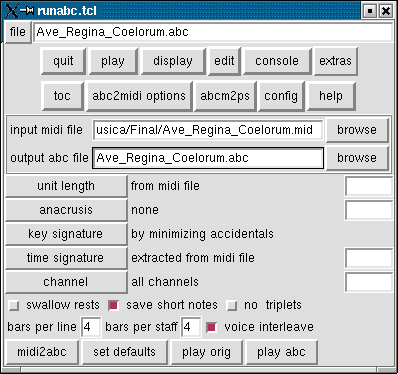
\includegraphics[scale=0.7]{runabc.png}
\caption{Converting a MIDI file to \ABC{} with \runabc{}.}
\label{fig:runabc}
\end{figure}

Don't expect to obtain perfect sources all the time! In fact, while
sheet music (be it written in \ABC{} or in any other format) can
always be translated into MIDI, the opposite does not always hold
true. Remember what I explained in Section~\ref{sec:midi}. For
example, you will see that trills are translated as sequences of short
notes; repeats will just duplicate measures; and many other problems.
Sometimes, note length will look crazy.

Bearing in mind that some of these limitations cannot be avoided, further
development is being planned to improve the output of \cmd{midi2abc}.

% -----

\subsection{Global Settings}

In a tune collection (i.e.\ a file containing several tunes), the same MIDI
settings could be shared by all or most tunes. Instead on inserting the same
\metacmd{MIDI} lines in each tune, it's possible to place them at the
beginning of the file; the parameters will apply to all tunes.

These parameters can be 

\begin{itemize}

  \item \metacmd{MIDI C}
  \item \metacmd{MIDI nobarlines}
  \item \metacmd{MIDI barlines}
  \item \metacmd{MIDI fermatafixed}
  \item \metacmd{MIDI fermataproportional}
  \item \metacmd{MIDI ratio}
  \item \metacmd{MIDI chordname}
  \item \metacmd{MIDI deltaloudness}
  
\end{itemize}

Obviously, these parameters may be overridden by \metacmd{MIDI} lines within
each tune.


% \subsection{\cmd{yaps}}

% This program is another \ABC{}-\ps{} converter. Its output quality and
% other features make it inferior to \abcm, and it will not be further
% discussed.

% -----

% \noteseparator

% -----

\section{Differences and Incompatibilities}

Unfortunately, \abcm{} and \abcmid{} are not completely compatible
with each other, because the first program accepts a more extended
syntax than the second. Moreover, it should be pointed out that some
indications only make sense in a printed score. Consequently, when
writing music in \ABC{} bear in mind that:

\begin{itemize}
  
  \item tremolo decorations don't produce audible effect;
  
  \item if a system change occurs in the middle of a piece, \abcmid{}
  gets lost and generates an incorrect MIDI file;
  
  \item in \field{U:} fields, \abcmid{} only accepts uppercase
  \car{H}{\ldots}\car{Z};
  
  \item {\ldots}there may be others. % TO DO: find them
  
\end{itemize}

Because of these small incompatibilities, we have the problem of writing
music that can be converted by both \abcm{} and \abcmid. In theory, we
should write two source files, one for \abcm{} and another for \abcmid{}:
this is obviously unacceptable. An alternative is to use the \abcpp{}
preprocessor, which is explained in the next section.

% -----

\noteseparator

% -----

\chapter{Converting}

\section{The \abcpp{} Preprocessor}
\label{sec:abcpp}

\lettrine{A}{} \emph{preprocessor} is a program that modifies a text
file, according to commands contained in the file. \abcpp{} is a
preprocessor expressly designed for \ABC{} files. It allows to

\begin{itemize}
  
  \item exclude or include parts of a piece according to specified
  conditions;
  
  \item define \emph{macros}, i.e.\ symbols and sequences of customised
  commands;
  
  \item rename commands, symbols, and notes;
  
  \item include parts of other files.
  
\end{itemize}

Needless to say, \abcpp{} is a command-line program. You run it specifying
the names of input and output files, and possibly defining \emph{symbols}.

% -----

\subsection{Basic Usage}

Let us look at an example. We will write a portable \ABC{} file, which
can be read correctly by \abcm{} and \abcmid. Save this source as
\file{test.abp}:

\begin{alltt}
X: 1
T: Test with abcpp
#ifdef ABCMIDI
T: (version for abc2midi)
Q: 1/4 = 120
#else
T: (version for abcm2ps)
Q: "Allegro" 1/4 = 120
#endif
K: C
cdef gabc'|c'bag fedc|
\end{alltt}

Note the lines that start in \car{\#}: these are \emph{directives}
(commands) to the preprocessor.

The first directive means: ``if the symbol ABCMIDI is defined,
then{\ldots}'' If the condition is true, the source continues with the next
two lines; otherwise, with the lines that follow the \cmd{\#else} directive.
The \cmd{\#endif} directive terminates the condition.

To convert the source to make it acceptable to \abcmid, we'll run \abcpp{}
with this command line:

\begin{verbatim}
abcpp -ABCMIDI test.abp test-midi.abc
\end{verbatim}

This way we define the \cmd{ABCMIDI} symbol, and a new \ABC{} file
will be created:

\begin{alltt}
X: 1
T: Test with abcpp
T: (version for abc2midi)
Q: 1/4 = 120
K: C
cdef gabc'|c'bag fedc|
\end{alltt}

If we run \abcpp{} without defining any symbols, we'll get the right
source for \abcm:

\begin{verbatim}
abcpp test.abp test-ps.abc
\end{verbatim}

\begin{alltt}
X: 1
T: Test with abcpp
T: (version for abcm2ps)
Q: "Allegro" 1/4 = 120
K: C
cdef gabc'|c'bag fedc|
\end{alltt}

Let us consider another example. Some \ABC{} applications don't
support invisible rests. To make it possible to use them portably, we
have to insert these lines in the source:

\begin{verbatim}
#ifdef OLD
#define !x! z
#else
#define !x! x
#endif
\end{verbatim}

In plain English: ``if the \cmd{OLD} symbol is defined, then turn the
\cmd{!x!} decoration into \car{z}; otherwise, \cmd{!x!} will become
\car{x}''. As you write the tune, you will use \cmd{!x!} to denote
invisible rests. When you convert the source for \abcm{} or other
programs, the \cmd{!x!} symbol will be turned into \car{x} or \car{z}
according to the presence of the symbol \cmd{OLD}.

% -----

\subsection{Advanced Usage}

% TO DO: fix this section

We have seen in Figure~\ref{fig:riuriuchiu} an example of \ABC{} file
in which the system changes. Unfortunately, \abcmid{} doesn't
correctly handle this source, because the number of voices is
variable.

Let us see how we can use \abcpp{} to obtain a version compatible with
\abcmid. The idea is to write \emph{all the voices}, even those that
contain only rests, then provide specific instructions for \abcm{} and
\abcmid. We will obtain a source where only voice 3 of parts A and C
is printed, while the second will contain all voices.

{\footnotesize
\begin{abcsource}
X: 1
T: Riu, riu, chiu, \bl{}241la guarda ribera!
C: Villancico (Spagna, sec. XVI)
M: C|
L: 1/2
Q: 1/2 = 240
#ifdef MIDI
P: ABCB
#endif
%%staves 3
V: 3 clef=treble-8 name="Tenor\bl{}nBass"
K: Am
% ONLY THE MEN
#ifdef MIDI
P: A
[V: 1] [M:none] z4               |z4z4    |z6    |
[V: 2] [M:none] z4               |z4z4    |z6    |
[V: 4] [K: Am octave=-1]\bl
[M:none] aaga             |f2ed2efg|a2a2z2|
#endif
[V: 3] [M:none] AAGA             |F2ED2EFG|A2A2z2|
w: Ri-u, ri-u, chi-u, \bl{}241la guar-da ri-be-ra!
%
#ifdef MIDI
[V: 1] z4               |z4z4    |z6    |
[V: 2] z4               |z4z4    |z6    |
[V: 4] aaga             |f2eg2gef|d2d2z2|
#endif
[V: 3] AAGA             |F2EG2GEF|D2D2z2|
w: Di\'os guar-d\'o el lo-bo de nue-stra cor-de-ra,
%
#ifdef MIDI
[V: 1] z4               |z4z4    |z4  |
[V: 2] z4               |z4z4    |z4  |
[V: 4] aaga             |f2eg2gef|d2d2|
#endif
[V: 3] AAGA             |F2EG2GEF|D2D2|
w: Di\'os guar-d\'o el lo-bo de nue-stra cor-de-ra.
% WOMEN AND MEN
#ifndef MIDI
%%staves [1 2 3 4]
V: 1 clef=treble   name="S" sname="S"
V: 2 clef=treble   name="A" sname="A"
V: 3 clef=treble-8 name="T" sname="T"
V: 4 clef=bass     name="B" sname="B"
#else
P: B
#endif
[V: 1]AAGA|F2ED2EFG |A2A2z2|
w: Ri-u, ri-u, chi-u, la guar-da ri-be-ra!
[V: 2]FFEC|D2EF2EDD |C2C2z2|
[V: 3]cccG|A2AA2ADD |E2E2z2|
w: Ri-u, ri-u, chi-u, la guar-da ri-be-ra!
[V: 4]ffcf|d2Ad2c_BB|A2A2z2|
%
[V: 1] z4      |AAGA|F2EF2FEE|D2D2z2|
w: Di\'os guar-d\'o el lo-bo de nue-stra cor-de-ra,
[V: 2] z2EE    |DCEC|D2CD2DCC|D2D2z2|
w: Di\'os guar-d\'o el lob', el lo-bo de nue-stra cor-de-ra,
[V: 3] ccBc    |A2BA|A2AA2AAA|A2A2z2|
w: Di\'os guar-d\'o el lo-bo, el lo-bo de nue-stra cor-de-ra,
[V: 4] aaga    |f2ef|d2Ad2dAA|d2d2z2|
%
[V: 1] z4  |AAGA|F2ED2DCC    |D2D2z2  |
w: Di\'os guar-d\'o el lo-bo de nue-stra cor-de-ra.
[V: 2] z2EE|DCEC|D2CA,2A,A,A,|A,2A,2z2|
w: Di\'os guar-d\'o el lob', el lo-bo de nue-stra cor-de-ra.
[V: 3] ccBc|A2BA|A2AF2FEE    |D2D2z2  |
w: Di\'os guar-d\'o el lo-bo, el lo-bo de nue-stra cor-de-ra.
[V: 4] aaga|f2ef|d2Ad2dAA    |d2d2z2  |
% ONLY THE MEN
#ifdef MIDI
P: C
[V: 1] z4  |z8      |z4|z4  |
[V: 2] z4  |z8      |z4|z4  |
[V: 4] aaga|f2eg2gef|d4|aaga|
#else
%%staves 3
#endif
[V: 3] AAGA|F2EG2GEF|D4|AAGA|
w: El lo-bo ra-bio-so la qui-so mor-der, mas Di\'os po-de-
%
#ifdef MIDI
[V: 1] z8      |z4|z4  |z8      |
[V: 2] z8      |z4|z4  |z8      |
[V: 4] f2feggef|d4|aaga|f2fedefg|
#endif
[V: 3] F2FEGGEF|D4|AAGA|F2FEDEFG|
w: ro-so la su-po de-fen-der; qui so-le ha-ce que no pu-die-sce pe-
%
#ifdef MIDI
[V: 1] z4|z4  |z8      |z4  |
[V: 2] z4|z4  |z8      |z4  |
[V: 4] a4|aaga|f2feggef|d2d2|
#endif
[V: 3] A4|AAGA|F2FEGGEF|D2D2|
w: car: ni~aun o-ri-gi-nal e-sta Vir-gen no tu-vie-ra.
\end{abcsource}
}

% -----

% \noteseparator

% -----

\section{\cmd{abc2abc}}

\lettrine{I}{t} is part of the \abcMID{} package. This command-line
program is used to modify the \ABC{} source in several ways.
\cmd{abc2abc} is followed by the name of the file to modify, and then
by one of these options:

\begin{description}
  
  \item [\cmd{-n} \parm{x}] reformats the source with \parm{x} measures
  per line.
  
  \item [\cmd{-t} \parm{n}] transposes the music by \parm{n} semitones.
  \parm{n} may be a negative number.
  
  \item [\cmd{-d}] doubles the note lengths.
  
  \item [\cmd{-v}] halves the note lengths.
  
  \item [\cmd{-V} \parm{x}] outputs only voice \parm{x} of a
  polyphonic file.\footnote{The program \cmd{abc2prt}
  (Section~\ref{sec:abcprt}) works better.}
  
  \item [\cmd{-X} \parm{n}] for a file with several pieces, renumbers the
  \field{X:} field starting with \parm{n}.
  
\end{description}

As usual, here is an example. Let us modify this scale:

\begin{abcsource}
X: 1
L: 1/4
K: C
CDEF|GABc|cdef|gabc'|c'cCz|
\end{abcsource}

starting \cmd{abc2abc} with this command line:

\begin{verbatim}
$ abc2abc cde.abc -n 2 -t 2
\end{verbatim}

that is, we are reformatting the source to get two measures per line
and transposing by two semitones up. This is what we obtain:

\begin{abcsource}
X:1
L:1/4
K:Eb
%
EFGA|Bcde|
efga|bc'd'e'|
e'eEz|
\end{abcsource}

The transposing feature will be extremely useful to players of
clarinet and other transposing instruments.

% -----

\noteseparator

% -----

\chapter{Other Possibilities}

% -----

\section{Inserting Music in Other Programs}
\label{sec:word}

\lettrine{S}{heet} music in \ps{} format can be easily converted to
other formats suitable for word processing, web pages, etc. In
practice, there are only two recommended formats: \graph{jpg} and
\graph{png}. The latter is the best.

To convert \ps{} to \graph{png}, Windows users can simply use GSview.
Select \entry{File}{Convert}, choose \texttt{png16} in the
\texttt{Device} field, then select the pages you wish to convert.

Resolution is a very important parameter. The higher the resolution,
the better the quality of the output; but the file size also grows
exponentially. A resolution of 300 dots per inch is fine.

Unix users could use the low-level Ghostscript interpreter. The
following script converts an input file to \graph{png}:

\begin{verbatim}
#!/bin/sh
FILE=$(basename $1 .ps)
gs -dNOPAUSE -q -dBATCH -sPAPERSIZE=a4 \
-sDEVICE=pnggray \
-dTextAlphaBits=4 -dGraphicsAlphaBits=4 \
-r300x300 \
-sOutputFile=$FILE-%003d.png \
$1
\end{verbatim}

A similar method is using \app{convert}, a command provided by the
ImageMagick package (\url{http://www.imagemagick.org/}). You use it as
in this example:

\begin{verbatim}
convert -density 300x300 file.ps file.png
\end{verbatim}

The \cmd{-density} parameter specifies the resolution.

% -----

% \noteseparator

% -----

\section{Inserting Music in \LaTeX}
\label{sec:latex}

This guide is written in \LaTeX, which you may want to use instead of
a word processor. To insert \ABC{} music in \LaTeX{} documents,
you have to decide whether your final format will be \ps{} or PDF.

In both cases, you will have to convert the score to \graph{eps}
(encapsulated \ps). This is done either by specifying the \cmd{-E}
switch in the \abcm{} command line, or using the command
\cmd{ps2epsi}. This one is part of Ghostscript. When you are done, you
will include the \app{graphicx} package in your document and include
the music as in this example:

\begin{verbatim}
\documentclass[a4paper,12pt]{article}
\usepackage{graphicx}
\begin{document}
This is some ABC music:

\medskip
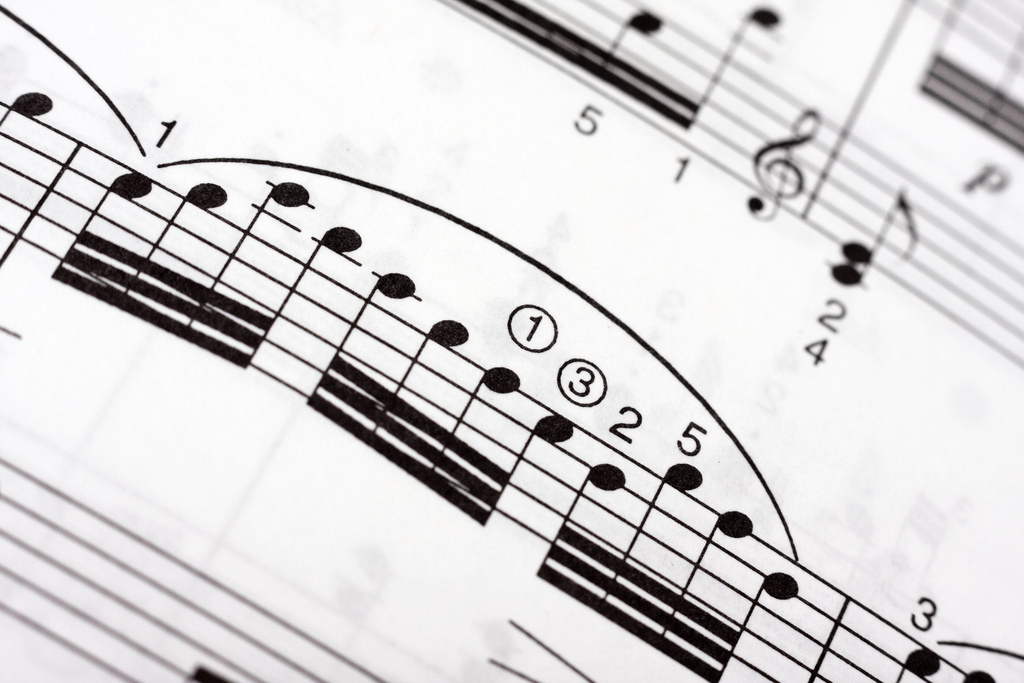
\includegraphics[width=\linewidth]{music.eps}
\end{document}
\end{verbatim}

If you wish to use \cmd{pdflatex}, you will have to convert the score
from \graph{eps} to PDF using \cmd{epstopdf}, then insert the PDF file
in the \LaTeX{} source.

% -----

\subsection{Using \file{abc.sty}}

Prof. Enrico Gregorio of University of Verona, Italy, has written a
package that enables the inclusion of \ABC{} code in \LaTeX{}
documents. The relevant archive, called \file{abc.zip}, can be freely
obtained from CTAN mirrors. Please see Section~\ref{sec:weblinks} for
details.

Once installed, the file \file{abc.sty} provides the following
facilities:

\begin{itemize}

  \item the \texttt{abc} environment
  
  \item the \texttt{\bl{}abcinput} command
  
  \item the \texttt{\bl{}abcwidth} parameter.

\end{itemize}

More explanations are included in the package documentation. This is a
sample \LaTeX{} document that employs \file{abc.sty}:

\begin{verbatim}
\documentclass[a4paper,12pt]{article}
\usepackage[generate,ps2eps]{abc}
\usepackage{mathptmx}

\begin{document}

\title{Example of ABC in \LaTeX{}}
\author{Guido Gonzato}
\date{}
\maketitle

This is a short piece. 

\medskip

\begin{abc}
X:4
T:Cronin's Hornpipe
R:hornpipe
S:Keenan and Glackin
E:7
M:C|
L:1/8
K:G
BA|GABc dBde|gage dega|bage dBGB|cABG A2BA|
GABc dBde|gage dega|bage dBAB|G2G2 G2:|
fg|afd^c d2ga|bged e2ga|(3bag  (3agf gedB|(3cBA AG AcBA|
GABc dBde|~g3e dega|bage dBAB|G2G2 G2:|
\end{abc}

\medskip

Let's now include a tune we have in the current directory as 
\file{tune.abc}:

\medskip

\abcinput{tune}

\end{document}
\end{verbatim}

% -----

% \noteseparator

% -----

\section{Converting Graphics to \graph{eps}}
\label{sec:jpgeps}

Very often, graphic files are in \graph{jpg}, \graph{gif} or
\graph{png} format. Converting such files into \graph{eps} files
suitable for inclusion with the \metacmd{EPS} command is best done
with yet another command-line program, \app{bmeps}. It is available
from \url{http://www.ctan.org/tex-archive/support/bmeps}; I suggest
that Windows users download the provided static binary.

\app{bmeps} is used as in this example:

\begin{verbatim}
$ bmeps -c myfile.png myfile.eps
\end{verbatim}

If you omit \cmd{-c}, the resulting \graph{eps} file will be in black
and white.

% -----

% \noteseparator

% -----

\section{Parts Extraction}
\label{sec:abcprt}

Another useful tool is \abcprt, which extract voices from polyphonic
sources. You use \abcprt{} to create new \ABC{} files containing the
single voices.

For example, let us suppose we want to extract the tenor part (voice
3) from the Ave Verum listed in Section~\ref{sec:format}. All you have
to do is run \abcprt{} this way:

\begin{verbatim}
abc2prt -3 aveverum.abc aveverum-3.abc
\end{verbatim}

A new \ABC{} file called \file{aveverum-3.abc}, containing only voice
3, will be created.

Needless to say, \abcprt{} is integrated in \jedabc{}.

% -----

% \noteseparator

% -----

\section{Limitations of \abcm}

Although it is a very powerful program, \abcm{} currently has a few
limitations to be aware of:

\begin{itemize}
  
  \item no manual control over symbol positioning;
  
  \item some formatting parameters cannot change within the same tune;
  
  \item doesn't support special notations like percussions or Gregorian
  Chant;
  
  \item {\ldots}
  
\end{itemize}

This list was longer some versions ago{\ldots} Most likely, the
missing features will be implemented in future releases.

% -----

% \noteseparator

% -----

\section{Final Comments}

I started with \ABC{} several years ago, and it's always been my
tool of choice whenever I needed to print or listen to a piece of
music. This manual started out as a list of notes I wrote for myself,
and it slowly grew to its present form. Since the \ABC{} software
is free, I decided it was only fair to release this manual for free as
well.

A big ``thank you!'' to the author of \abcm, Jean-Fran\c cois Moine,
for writing such a beautiful and useful program; to Michael Methfessel
for writing the original \app{abc2ps}; to James Allwright for writing
the original \abcMID{}, and to Seymour Schlien for maintaining and
improving it; to Chris Walshaw for creating \ABC{}; to Norman Schmidt
who helped me translating parts of this manual into English.

Thanks to my friend Sandro Pasqualetto and to Gianni Cunich for their
suggestions on how to improve this guide. Last but not least, thanks
to all people who contribute to \ABC!

% -----

\subsection{Please, Make a Donation{\ldots}}

I say again, this manual is free. That said, if the results of my work
on \ABC{} are useful to you, it would be a good thing if you made a
donation. I used to ask for a little amount of money, which I don't
need anymore now that the mortgage's over. So: please make a donation
to a charity of your choice, and let me know. You will gain some good
karma.

May I ask that you send me a postcard, too? I'm especially fond of
natural landscapes. Mountain views or geology images will make my day.

This is my home address: Guido Gonzato, Via Monte Ortigara 2/a, 37126
Verona, Italy.

Thank you so much!

% -----

\subsection{In Loving Memory of Annarosa Del Piero, 1930--2000}

I had the privilege to be a friend of Annarosa's, without whom I would
be a different person.

No rhetoric, Annarosa was unique. She profoundly loved and enjoyed art
and music. She shared her love with me when I was just a kid, giving
me records of opera arias as presents. She took me by train to visit
Venice for the first time in my life, and she introduced me to the
beauty of the mountains.

She confronted her fatal illness with courage and dignity. Till the
end she listened to her favourite music, till the end she gave me
beautiful records of operas as present. This guide is dedicated to her
memory: a tiny leaf born from the seed she throwed when she had a
six-year-old kid listen to Rigoletto, so many years ago. Ciao,
Annarosa.

\noteseparator

% ----- Appendix

\appendix
\chapter{Bits \& Pieces}

% -----

\section{Web Links}
\label{sec:weblinks}

The \ABCPLUS{} home page:

\url{http://abcplus.sourceforge.net}

The original \ABC{} page:

\url{http://www.abcnotation.com}

The \ABC{} Project page:

\url{http://abc.sourceforge.net/}

The \abcm{} home page:

\url{http://moinejf.free.fr}

The \abcmid{} home page and user guide:

\url{http://ifdo.pugmarks.com/~seymour/runabc/top.html}

\url{http://ifdo.pugmarks.com/~seymour/runabc/abcguide/abc2midi_guide.html}

Hudson Lacerda's \ABC{} page, including advanced customisation and
\ps{} new routines:

\url{http://hudsonlacerda.webs.com/}

The Folkinfo web-based \ABC{} converter:

\url{http://www.folkinfo.org/songs/abcconvert.php}

Abctab2ps is an almost complete implementation of \ABCPLUS{} that
supports tablatures for lute:

\url{http://www.lautengesellschaft.de/cdmm/}

The Philip's Music Writer home page is about a powerful and
easy-to-use textual music notation format, which could be a valuable
alternative to \ABC:

\url{http://www.quercite.com/pmw.html}

Lilypond is another high-quality music notation format, very powerful
but rather complex:

\url{http://lilypond.org/web/}

The \file{abc} package for \LaTeX:

\url{http://www.ctan.org/tex-archive/macros/latex/contrib/abc/}

Finally, the MusiX\TeX{} home page. This is a \TeX{}-based, very
complex notation that spurred the creation of two spinoffs, PMX and
M-Tx:

\url{http://icking-music-archive.org/}

% -----

% If you need to print tablatures for guitar, lute, and other string
% instruments, you will have to use a program similar to \abcm, called
% \abctab.


\section{\ABC{} Fields}

% Table~\ref{tab:campi} lists all \ABC{} language fields.

% \begin{table}[hbtp]
\begin{center}
\begin{tabular}{lll}
  \toprule % \hline
  \textbf{Field} & \textbf{Where} & \textbf{Notes and Example} \\
  \midrule % \hline
  A: & header & Area. \field{A:Liverpool} \\
  B: & header & Book. \field{B:Groovy Songs} \\
  C: & header & Composer. \field{C:The Beatles} \\
  D: & header & Discography. \field{D:The Beatles Complete Collection} \\
  d: & body & Decorations. \field{d:!pp! * * !mf! * !ff!} \\
  F: & header & File name. \field{F:http://www.beatles.org/help.abc} \\
  G: & header & Group. \field{G:guitar} \\
  H: & header & History. \field{H:This song was written...} \\
  I: & header & Information. \field{I:lowered by a semitone} \\
  I: & body & Meta-command. \field{I:MIDI program 2 32} \\
  K: & last in header & Key. \field{K:C} \\
  L: & header, body & Note length. \field{L:1/4} \\
  M: & header, body & Metre. \field{M:3/4} \\
  N: & header & Notes. \field{N:See also...} \\
  O: & header & Origin. \field{O:English} \\
  P: & header, body & Part. \field{P:Start} \\
  Q: & header, body & Tempo. \field{Q:1/2=120} \\
  R: & header & Rhythm. \field{R:Reel} \\
  S: & header & Source. \field{S:Collected in Liverpool} \\
  s: & body & Decorations. \field{s:!pp! * * !mf! * !ff!} \\
  T: & second in header & Title. \field{T:Help!} \\
  U: & header & User defined. \field{U:T=!trill!} \\
  V: & header, body & Voice. \field{V:1} \\
  W: & body & Lyrics at end. \field{W:Help! I need...} \\
  w: & body & inline lyrics. \field{w:Help! I need...} \\
  X: & start of header & Index number. \field{X:1} \\
  Z: & header & Transcription notes. \field{Z:Transcribed by ear} \\
  \bottomrule % \hline
\end{tabular}
% \caption{Fields of the \ABC{} language.}
\label{tab:campi}
\end{center}
% \end{table}

% -----

% \noteseparator

% -----

\section{Glossary}
\label{sec:help}

\begin{description}
  
  \item [editor:] a program to write ``ASCII text'', that is with no
  special format. Windows' Notepad (ugh), \app{emacs} and \app{vim}
  are some well-known editors.
  
  \item [font:] type of character; for instance, Times or Helvetica.
  
  \item [GPL:] a software license that disciplines the use of many
  programs available from the Internet. Briefly, a GPL'ed program can
  be freely used, modified and shared, without having to pay for it.
  Please visit \url{http://www.gnu.org/} for more details.
  
  \item [MIDI:] roughly speaking, the audible equivalent of sheet music.
  You can listen to a MIDI file using dedicated players.
  
  \item [PDF:] file format invented by Adobe, very common on the
  Internet to distribute documentation. It is a spinoff of \ps.
  
  \item [\ps:] file format invented by Adobe. Unlike graphic files
  like \graph{jpg}, \graph{png} or others, \ps{} is a \emph{vector}
  format. This means that one can magnify the image at will, without
  losing in details.
  
  \item [system:] set of staves relative to the instruments that play
  together in a musical piece.
  
  \item [string:] word, set of characters.
  
\end{description}

% -----

% \noteseparator

% -----

\section{Character Sets}
\label{sec:isolatin}

% TO DO: probably this section will go away

One of the nicest things in the world is diversity. Different
languages use different characters, but this can lead to
incompatibility problems when, say, an Italian musician wants to send
his or her American friend an \ABC{} source.

Fortunately, there exist a character set called ISO 8859-1 (Latin1)
that includes accented characters used by many languages: all of
central Europe, and all English-speaking countries. These characters
have an ASCII code between 160 and 255, and can be typed as sequences
\car{\bl{}xxx} when not available on the keyboard.

The Latin1 characters and the corresponding octal code are shown
below. I \emph{recommend} that you use the \car{\bl{}xxx} sequence
even if you do have these characters on your keyboard, because this
makes the source more portable.

\score{isolatin}

% Eastern European languages such as Czech, Hungarian, Polish, Romanian,
% Croatian, Slovak, Slovenian, and Serbian use the ISO-8859-2 (Latin2)
% character set:

% \score{isolatin2}

% -----

% \noteseparator

% -----

\section{Formatting Commands}
\label{sec:commands}

Command parameters will be specified as follows:

\medskip

\begin{center}
\begin{tabular}{ll}
  \toprule % \hline
  \textbf{Parameter} & \textbf{Type} \\
  \midrule % \hline
  \emph{len\-gth} & unit length indicated in \texttt{cm},
     \texttt{in} or \texttt{pt}  \\
  \emph{text} & generic text \\
  \emph{logical} & logical value, \texttt{yes} or \texttt{no}, or 1 or 0 \\
  \emph{int} & integer number \\
  \emph{float} & number with decimals \\
  \emph{str} & character string \\
  \bottomrule % \hline
\end{tabular}
\end{center}


% ----- page format

\subsection{Page Format}

These commands set the page geometry.

\begin{description}

  \item[\metacmd{botmargin} \parm{len\-gth}:] sets the page bottom margin
  to \parm{len\-gth}.

  \item[\metacmd{footer} \parm{text}:] sets the text to be printed as
  footer on each page. % TO BE EXPANDED

  \item[\metacmd{header} \parm{text}:] sets the text to be printed as
  header on each page. % TO BE EXPANDED

  \item[\metacmd{indent} \parm{len\-gth}:] sets the indentation for
  the first line or system to \parm{len\-gth}.

  \item[\metacmd{landscape} \parm{logical}:] if 1, sets the page
  layout as landscape.

  \item[\metacmd{leftmargin} \parm{len\-gth}:] sets the page left
  margin to \parm{len\-gth}.
  
  \item[\metacmd{multicol} \parm{command}:] defines columns.
  \parm{command} may be \cmd{start}, \cmd{new}, and \cmd{end}. See
  Section~\ref{sec:multicol} for details.

  \item[\metacmd{pageheight} \parm{len\-gth}:] sets the page height to
  \parm{len\-gth}. For European A4 paper, the right value is
  \cmd{29.7cm}; for US Letter, \cmd{11in}.

  \item[\metacmd{pagewidth} \parm{len\-gth}:] sets the page width to
  \parm{len\-gth}. For European A4 paper, the right value is
  \cmd{21cm}; for US Letter, \cmd{8.5in}.

  \item[\metacmd{rightmargin} \parm{len\-gth}:] sets the page right
  margin to \parm{len\-gth}.

  \item[\metacmd{staffwidth} \parm{len\-gth}:] used as an alternative
  to the commands \metacmd{page\-height} and \metacmd{pa\-ge\-width}.

  \item[\metacmd{topmargin} \parm{len\-gth}:] sets the page top margin
  to \parm{len\-gth}.

\end{description}

% ----- text

\subsection{Text}

These commands are used to write text lines within a tune and between
tunes. Fonts and spacing are set with other commands that we will
examine later on.

\begin{description}

  \item [\metacmd{begintext{\ldots}\%\%endtext}]: the pair
  \metacmd{begintext} and \metacmd{endtext} includes a group of text
  lines. These lines will be printed. If no text follows
  \metacmd{}, the line is a paragraph separator. For example:

\begin{verbatim}
%%begintext
%%Spanish folk song, usually
%%accompanied by guitar and cymbals.
%%endtext
\end{verbatim}

  The command \metacmd{begintext} can be given a parameter to change the
  text alignment:

  \begin{description}

    \item [\metacmd{begintext obeylines}] prints text as is;

    \item [\metacmd{begintext fill}] (or \cmd{ragged}) formats the text to
    the page margins;

    \item [\metacmd{begintext justify}] (or \cmd{align}) as above, but
    aligns to the page right margin;

    \item [\metacmd{begintext skip}] ignores the following lines.

  \end{description}

  \item [\metacmd{center} \parm{text}:] centers the following text.

  \item [\metacmd{text} \parm{text}:] writes the following text. For
  example:

\begin{verbatim}
%%text Spanish folk song
\end{verbatim}

  \item [\metacmd{textoption} \parm{int}:] sets the default text
  option to be used between \metacmd{be\-gin\-text} and \metacmd{end\-text},
  or in \metacmd{EPS} files. The parameter can be a digit or a corresponding
  string: 0 or \cmd{obeylines}), 1 (\cmd{justify}), 2 (\cmd{fill}), 3
  (\cmd{center}), 4 (\cmd{skip}), 5 (\cmd{right}). If the option is 4
  (\cmd{skip}), no text or EPS is output.


\end{description}

% ----- font

\subsection{Fonts}
\label{sec:fonts}

These commands specify the character fonts used in various parts of a
score. Please note that the common True Type fonts used by Windows
\emph{are not the same fonts} used by \abcm. In fact, \abcm{} uses the
\ps{} fonts, provided for and managed by Ghostscript.

Standard fonts are shown in Appendix~\ref{sec:fontlist}. I remind you that
indications for adding new fonts are given in Section~\ref{sec:addfonts}.

\begin{description}

  \item[\metacmd{annotationfont} \parm{string}:] font of 
  annotations.
  
  \item[\metacmd{composerfont} \parm{string}:] \field{C:} field font.

  \item[\metacmd{footerfont} \parm{string}:] font of \metacmd{footer}
  lines.

  \item[\metacmd{font} \parm{string}:] declares a font for later usage.

  \item[\metacmd{gchordfont} \parm{string}:] guitar chords font.

  \item[\metacmd{headerfont} \parm{string}:] font of \metacmd{header}
  lines.
  
  \item[\metacmd{historyfont} \parm{string}:] font of \field{H:}
  field.

% TO DO - inconsistent!

  \item[\metacmd{infofont} \parm{string}:] text font in \field{I:} fields.
  
  \item[\metacmd{measurefont} \parm{string} \optparm{box}:] text font of
  measure numbers. If the word \cmd{box} is present, a box is drawn around
  the measure number.

  \item[\metacmd{partsfont} \parm{string}:] \field{P:} fields font.
  
  \item[\metacmd{repeatfont} \parm{string}:] font of repeat numbers or text.
  
  \item[\metacmd{setfont-}\parm{int} \parm{string} \parm{int}:] sets an
  alternate font for strings. In most strings, the current font may be
  changed by \cmd{\$n} (n = 1, 2, 3, 4). \cmd{\$0} resets the font to the
  default value.

  \item[\metacmd{subtitlefont} \parm{string}:] font of the second \field{T:}
  field.

  \item[\metacmd{tempofont} \parm{string}:] tempo font.

  \item[\metacmd{textfont} \parm{string}:] text font in \metacmd{text}
  lines.
  
  \item[\metacmd{titlecaps} \parm{logical}:] if true, writes the title in
  capital letters.

  \item[\metacmd{titlefont} \parm{string}:] font of the first \field{T:}
  field.

  \item[\metacmd{titleformat} \parm{string}:] defines the format of the tune
  title. This format overrides \metacmd{ti\-tle\-left},
  \metacmd{infoline}, and \metacmd{composerspace}. See
  Section~\ref{sec:titles} for examples. % TO BE EXPANDED.

  \item[\metacmd{titleleft} \parm{logical}:] if true, writes the title
  left-aligned instead of centered.

  \item[\metacmd{voicefont} \parm{string}:] font of voice names.

  \item[\metacmd{vocalfont} \parm{string}:] font of the text in \field{w:}
  lines.

  \item[\metacmd{wordsfont} \parm{string}:] font of the text in \field{W:}
  lines.

\end{description}

% ----- spacing

\subsection{Spacing}

These commands specify spacing between score elements.

\begin{description}

  \item[\metacmd{barsperstaff} \parm{int}:] tries to typeset the score
  with \parm{int} bars on each line.

  \item[\metacmd{breakoneoln} \parm{logical}:] if true, treats an end of
  line as if it were a space (i.e.\ breaks note beams).

  \item[\metacmd{composerspace} \parm{len\-gth}:] sets the vertical space
  before the composer to \parm{len\-gth}.
  
  \item[\metacmd{gracespace} \parm{float} \parm{float} \parm{float}:]
  defines the space before, within and after grace no\-tes.

  \item[\metacmd{infospace} \parm{len\-gth}:] sets the vertical space
  before the infoline to \parm{len\-gth}.

  \item[\metacmd{lineskipfac} \parm{float}:] sets the factor for spacing
  between lines of text to \parm{float}.

  \item[\metacmd{maxshrink} \parm{float}:] sets how much to compress
  horizontally when staff breaks are chosen automatically. \parm{float}
  must be between 0 (don't shrink) and 1 (full shrink).

  \item[\metacmd{maxstaffsep} \parm{len\-gth}:] sets the maximum
  vertical space between staves.
  
  \item[\metacmd{maxsysstaffsep} \parm{len\-gth}:] sets the maximum
  vertical space between systems.

  \item[\metacmd{musicspace} \parm{len\-gth}:] sets the vertical space 
  before the first staff to \parm{len\-gth}.

  \item [\metacmd{newpage}:] sets a page break.
  
  \item[\metacmd{notespacingfactor} \parm{float}:] sets the proportional
  spacing of notes. The default value is 1.414 ($\sqrt{2}$); 1 makes all
  notes equally spaced.

  \item[\metacmd{parskipfac} \parm{float}:] sets the factor for spacing
  between parts to \parm{float}.

  \item[\metacmd{partsspace} \parm{len\-gth}:] sets the vertical space 
  before a new part to \parm{len\-gth}.

  \item[\metacmd{scale} \parm{float}:] sets the music scale factor to
  \parm{float}.

  \item [\metacmd{sep}:] prints a centered separator (a short line).

  \item [\metacmd{sep} \parm{len\-gth1} \parm{len\-gth2} \parm{len\-gth3}:] 
  prints a separator of len\-gth \parm{len\-gth3}, with spacing
  \parm{le\-ngth1} above and \parm{len\-gth2} below.

  \item[\metacmd{slurheight} \parm{float}:] sets the slur height factor;
  lesser than 1 flattens the slur, greater than 1 expands it.

  \item[\metacmd{staffbreak} \parm{len\-gth} \optparm{``f''}:] sets a
  \parm{len\-gth}-long break (gap) in the current staff. If the letter
  ``f'' is present, the staff break is forced even if it occurs at the
  beginning or end of a line.
  
  \item[\metacmd{staffsep} \parm{len\-gth}:] sets the vertical space between
  different systems to \parm{len\-gth}.

  \item[\metacmd{stretchlast} \parm{logical}:] stretches the last staff of
  the tune when underfull.

  \item[\metacmd{stretchstaff} \parm{logical}:] stretches underfull staves
  across page.

  \item[\metacmd{subtitlespace} \parm{len\-gth}:] sets the vertical space
  before the subtitle to \parm{len\-gth}.

  \item[\metacmd{sysstaffsep} \parm{len\-gth}:] sets the vertical space between
  staves in the same system to \parm{len\-gth}.

  \item[\metacmd{textspace} \parm{len\-gth}:] sets the vertical space before
  texts to \parm{len\-gth}.

  \item[\metacmd{titlespace} \parm{len\-gth}:] sets the vertical space before
  the title to \parm{len\-gth}.

  \item[\metacmd{topspace} \parm{len\-gth}:] sets the vertical space at the
  top of a tune to \parm{len\-gth}. Note that a tune may begin with
  \metacmd{text} commands before the title.

  \item[\metacmd{vocalspace} \parm{len\-gth}:] sets the vertical space before
  the lyrics under staves to \parm{len\-gth}.

  \item [\metacmd{vskip} \parm{h}:] adds \parm{h} vertical space. \parm{h}
  may be a negative value.
  
  \item[\metacmd{wordsspace} \parm{len\-gth}:] sets the vertical space before
  the lyrics at end of the tune to \parm{len\-gth}.

\end{description}

% ----- other

\subsection{Other Commands}
\label{sec:othercmd}

Miscellaneous commands are grouped in this section.

\begin{description}

  \item[\metacmd{abc2pscompat} \parm{logical}]: if true, reverts to the old
  metod of dealing with notes in bass and other clefs. Please see
  Section~\ref{sec:bassclef}.

  \item[\metacmd{alignbars} \parm{int}:] aligns the bars of the next 
  \parm{int} lines of music. It only works on single-voice tunes.

  \item[\metacmd{aligncomposer} \parm{int}:] specifies where to 
  print the composer field. A negative value me\-ans ``on the left'',
  0 means ``centre'', and a positive value means ``on the right''.
  
  \item[\metacmd{autoclef} \parm{logical}:] if true, prints clefs and
  possibly clef changes when no clef is defined in \field{K:} or \field{V:}.

  \item[\metacmd{barnumbers} \parm{int}:] same as \metacmd{measurenb}, 
  see below.
  
  \item[\metacmd{beginps}--\metacmd{endps}:] start/end of a \ps{} sequence.
  
  \item[\metacmd{bstemdown} \parm{logical}:] if true, the stem of
  the note on the middle of the staff goes downwards. Otherwise, it goes
  upwards or downwards according to the previous note.
  
  \item[\metacmd{comball} \parm{logical}:] if true and 
  \metacmd{combinevoices} is set, combines voices in all cases.
  
  \item[\metacmd{combinevoices} \parm{logical}:] if true, notes
  of same duration that belong to voices of the same staff are combined
  producing chords. It does not apply when note pitches are in unison,
  inverted or differ by a second.
  
  \item[\metacmd{continueall} \parm{logical}:] ignores the line breaks in
  tune if true. It's the equivalent of the \cmd{-c} command line flag.
  
  \item[\metacmd{contbarnb} \parm{logical}:] if true, the bar number
  of the second repeat(s) is reset to the number of the first repeat. If
  false, bars are sequentially numbered.
  
  \item[\metacmd{dateformat} \parm{string}:] defines the format of
  date and time. Default is \cmd{\%b \%e, \%Y \%H:\%M}. The fields specify,
  respectively: abbreviated month name (Jan--Dec), day of month (1--31),
  year, hour (0--23), minute (0--59).

  \item[\metacmd{deco} \parm{string1} \parm{int1} \parm{string2} \parm{int2}
  \parm{int3} \parm{int4} \parm{string3}:] adds a new decoration. Details
  are explained in Section~\ref{sec:decopers}.
  
  \item[\metacmd{dynalign} \parm{logical}:] if true, horizontally 
  aligns the dynamic marks.

  \item[\metacmd{EPS} \parm{string3}:] includes an external EPS
  file in the score.

  \item[\metacmd{encoding} \parm{int}:] (for expert users) sets the
  language encoding to ISO-Latin\parm{int}, which may range from 0 to 6.
  The value 0 is the same as 1, but the \ps{} encoding table is not output.

  \item[\metacmd{exprabove} \parm{logical}:] draws the expression
  decorations above the staff. If neither \cmd{expr\-above} nor
  \cmd{exprbelow} are true, the expression decorations are drawn above the
  staff if there are lyrics on the staff, below otherwise. \cmd{exprabove}
  takes precedence over \cmd{expr\-below}.

  \item[\metacmd{exprbelow} \parm{logical}:] draws the expression
  decorations below the staff.

  \item[\metacmd{flatbeams} \parm{logical}:] if true, forces flat beams in
  bagpipe tunes (\field{K:HP}).

  \item[\metacmd{freegchord} \parm{logical}:] if true, prevents the
  characters \car{\#}, \car{b} and \car{=} from being displayed as sharp,
  flat and natural sign in guitar chords. When this flag is set, displaying
  accidental may be forced escaping the characters (e.g.\
  \car{\textbackslash{}\#}.)
  
  \item[\metacmd{format} \parm{string}:] reads the format file specified
  as parameter.

  \item[\metacmd{gchordbox} \parm{logical}:] draws a box around accompaniment
  chords.
  
  \item[\metacmd{graceslurs} \parm{logical}:] draws slurs on grace notes.
  
  \item[\metacmd{hyphencont} \parm{logical}:] if true and if lyrics
  under the staff end with a hyphen, puts a hyphen in the next line.
  
  \item[\metacmd{infoline} \parm{logical}:] if true, displays the rhythm
  and the origin on the same line, plus the \field{A:} field.
  
  \item[\metacmd{infoname} \parm{string} \parm{string}:] defines the
  fields to be printed when \metacmd{writehistory} is true.

  \item[\metacmd{measurenb} \parm{int}:] draws the measure number
  every \parm{int} bars.

  \item[\metacmd{measurebox} \parm{logical}:] draws a box around measure
  numbers.

  \item[\metacmd{measurefirst} \parm{int}:] starts numbering the
  measures from \parm{int}.

  \item[\metacmd{musiconly} \parm{logical}:] if true, doesn't output the
  lyrics.

  \item[\metacmd{oneperpage} \parm{logical}:] outputs one tune per page.

  \item[\metacmd{partsbox} \parm{logical}:] draws a box around part names.

  \item[\metacmd{postscript} \parm{string}:] a series of these commands
  lets the user add a new \ps{} routine, or change an existing one.

  \item[\metacmd{printparts} \parm{logical}:] prints the part indications
  (\field{P:}).

  \item[\metacmd{printtempo} \parm{logical}:] prints the tempo indications
  (\field{Q:}).
  
  \item[\metacmd{pslevel} \parm{int}:] specifies the \ps{} level (1, 2,
  or 3).
  
  \item[\metacmd{repbra} \parm{logical}:] if false, prevents
  displaying repeat brackets for the current voice.
  
  \item[\metacmd{score} \parm{string}:] like \metacmd{staves}, but
  with a different behaviour regarding bars. See
  Section~\ref{sec:staves} for details.
  
  \item[\metacmd{setbarnb} \parm{int}:] sets the number of the next measure.
  
  \item[\metacmd{setdefl} \parm{logical}:] if true, outputs some
  indications about the note/chord and/or decorations for
  customization purposes. These indications are stored in the
  PostScript variable ``defl''.
  
  \item[\metacmd{shifthnote} \parm{logical}:] in multivoice
  tunes, when voices go to unison with a white and a black note (say, a half
  and a quarter note), only the black note head is printed. When this flag
  is set, a note shift is done and both are printed.

  \item[\metacmd{shiftunisson} \parm{logical}:] if true, shifts note heads
  that belong to different voices that are in unison. It applies to dotted
  notes and notes shorter than minim.

  \item[\metacmd{splittune} \parm{logical}:] if true, splits tunes that do
  not fit in a single page.

  \item[\metacmd{squarebreve} \parm{logical}:] displays ``brevis'' notes 
  in square format.

  \item[\metacmd{straightflags} \parm{logical}:] prints straight flags on
  stems in bagpipe tunes.
  
  \item[\metacmd{staff} \parm{int}:] prints the next symbols of
  the current voice on the \parm{int}-th staff.
  
  \item[\metacmd{staffnonote} \parm{logical}:] if false, staves with no
  notes are not printed.
  
  \item[\metacmd{staves} \parm{string}:] defines how staves are to be
  printed. See Section~\ref{sec:staves} for details.
  
  \item[\metacmd{stemheight} \parm{float}:] sets the stem height to
  \parm{float}.

  \item[\metacmd{tablature} :] TO BE WRITTEN

  \item[\metacmd{timewarn} \parm{logical}:] if true, if a time signature
  occurs at the beginning of a music line, a cautionary time signature is
  added at the end of the previous line.
  
  \item[\metacmd{titletrim} \parm{logical}:] if true, move the last word 
  of a title to the head if it starts with a capital letter and it's
  preceded by a space and a comma.

  \item[\metacmd{tuplets} \parm{int1} \parm{int2} \parm{int3}:]
  defines how tuplets are to be drawn. See Section~\ref{sec:tuplets} for
  details.

  \item[\metacmd{vocalabove} \parm{logical}:] draws the vocals above the
  staff.

  \item[\metacmd{withxrefs} \parm{logical}:] prints the \field{X:} number
  in the title.

  \item[\metacmd{writehistory} \parm{logical}:] outputs notes, history,
  etc.

\end{description}

% -----

% \noteseparator

% ----- abc2midi commands

\section{\abcMID{} commands}
\label{sec:midcmds}

Some of these commands will only make sense to advanced users who have
some experience with MIDI files. In a few cases, explanations are
taken from the \file{abcguide.txt} file included in the \abcMID{}
archive.

\begin{description}

  \item [\metacmd{MIDI barlines}:] turns off \metacmd{nobarlines}.

  \item [\metacmd{MIDI bassprog} \parm{int}:] sets the MIDI instrument
  for the bass notes in accompaniment chords to \parm{int} (0--127).

  \item [\metacmd{MIDI bassvol} \parm{int}:] sets the velocity (i.e., 
  volume) of the bass notes to \parm{int} (0--127).

  \item [\metacmd{MIDI beat} \parm{int1} \parm{int2} \parm{int3} 
  \parm{int4}:] controls the volumes of the notes in a measure. The
  first note in a bar has volume \parm{int1}; other ``strong'' notes
  have volume \parm{int2} and all the rest have volume \parm{int3}.
  These values must be in the range 0--127. The parameter \parm{int4}
  determines which notes are ``strong''. If the time signature is x/y,
  then each note is given a position number \emph{k} = 0, 1, 2{\ldots}
  x-1 within each bar. If \emph{k} is a multiple of \parm{int4}, then
  the note is ``strong''.
  
  \item [\metacmd{MIDI beataccents}:] reverts to normally emphasised
  notes. See also \metacmd{MIDI no\-beat\-ac\-cents}.
  
  \item [\metacmd{MIDI beatmod} \parm{int}:] increments the velocities
  as defined by \metacmd{MIDI beat}

  \item [\metacmd{MIDI beatstring} \parm{string}:] similar to
  \metacmd{MIDI beat}, but indicated with an \cmd{fmp} string.

  \item [\metacmd{MIDI c} \parm{int}:] specifies the MIDI pitch which
  corresponds to \car{C}. The default is 60. This number should
  normally be a multiple of 12.

  \item [\metacmd{MIDI channel} \parm{int}:] selects the melody channel
  \parm{int} (1--16).

  \item [\metacmd{MIDI chordattack} \parm{int}:] delays the start
  of chord notes by \parm{int} MIDI units.

  \item [\metacmd{MIDI chordname}
  \parm{string int1 int2 int3 int4 int5 int6}:] defines new chords or
  rede\-fi\-nes existing ones as was seen in Section~\ref{sec:newacc}.

  \item [\metacmd{MIDI chordprog} \parm{int}:] sets the MIDI
  instrument for accompaniment chords to \parm{int} (0--127).

  \item [\metacmd{MIDI chordvol} \parm{int}:] sets the volume (velocity)
  of the chord notes to \parm{int} (0--127).

  \item [\metacmd{MIDI control} \parm{bass/chord} \parm{int1 int2}:]
  generates a MIDI control event. If \metacmd{control} is followed by
  \parm{bass} or \parm{chord}, the event apply to the bass or chord
  channel, otherwise it will be applied to the melody channel.
  \parm{int1} is the MIDI control number (0--127) and \parm{int2} the
  value (0--127).

  \item [\metacmd{MIDI deltaloudness} \parm{int}:] by default, 
  \cmd{!crescendo!} and \cmd{!dimuendo!} modify the be\-at variables
  \parm{vol1} \parm{vol2} \parm{vol3} 15 volume units. This command
  allows the user to change this default.

  \item [\metacmd{MIDI drone} \parm{int1 int2 int3 int4 int5}:]
  specifies a two-note drone accompaniment. \parm{int1} is the drone
  MIDI instrument, \parm{int2} the MIDI pitch 1, \parm{int3} the MIDI
  pitch 2, \parm{int4} the MIDI volume 1, \parm{int5} the MIDI volume
  2. Default values are 70 45 33 80 80.

  \item [\metacmd{MIDI droneoff}:] turns the drone accompaniment off.
  
  \item [\metacmd{MIDI droneon}:] turns the drone accompaniment on.

  \item [\metacmd{MIDI drumbars} \parm{int}:] specifies the number of
  bars over which a drum pattern string is spread. Default is 1.

  \item [\metacmd{MIDI drum} \parm{str}
  \parm{int1 int2 int3 int4 int5 int6 int7 int8}:] generates a drum
  accom\-pa\-ni-ment pattern, as described in Section~\ref{sec:rhythm}.

  \item [\metacmd{MIDI drummap} \parm{str} \parm{int}:] associates 
  the note \parm{str} (in \ABC{} notation) to the a percussion
  instrument, as listed in Section~\ref{sec:perc}.

  \item [\metacmd{MIDI drumoff}] turns drum accompaniment off.
  
  \item [\metacmd{MIDI drumon}] turns drum accompaniment on.

  \item [\metacmd{MIDI fermatafixed}:] expands a \cmd{!fermata!} by
  one unit len\-gth; that is, \cmd{HC3} becomes \cmd{C4}.
  
  \item [\metacmd{MIDI fermataproportional}:] doubles the len\-gth of a
  note preceded by \cmd{!fermata!}; that is, \cmd{HC3} becomes
  \cmd{C6}. \abcmid{} does this by default.

  \item [\metacmd{MIDI gchordbars} \parm{str}:] spreads the gchord
  string over \parm{n} consecutive bars of equal length. The gchord
  string should be evenly divisible by \parm{n} or else the gchords
  will not work
  properly. % COPIED FROM ABCMIDI DOC

  \item [\metacmd{MIDI gchord} \parm{str}:] sets up how guitar chords
  are generated. Please see Section~\ref{sec:midichords}.

  \item [\metacmd{MIDI gchordoff}:] turns guitar chords off.

  \item [\metacmd{MIDI gchordon}:] turns guitar chords on.

  \item [\metacmd{MIDI grace} \parm{float}:] sets the fraction of the
  next note that grace notes will take up. \parm{float} must be a
  fraction such as \texttt{1/6}.

  \item [\metacmd{MIDI gracedivider} \parm{int}:] sets the grace note
  len\-gth as 1/\parm{int}th of the following note.

  \item [\metacmd{MIDI makechordchannels} \parm{int}:] this is a very 
  complex command used in chords containing microtones. Please consult the
  \abcMID{} documentation.

  \item [\metacmd{MIDI nobarlines}:] normally, an accidental applied
  to a note also applies to other equal notes until the next bar. By
  using this command, the accidental will apply to the following note
  only.

  \item [\metacmd{MIDI nobeataccents}:] forces the \parm{int2} volume
  (see \metacmd{MIDI beat}) for each note in a bar, regardless of
  their position.

  \item [\metacmd{MIDI noportamento}:] turns off the portamento
  controller on the current channel.

  \item [\metacmd{MIDI pitchbend} \parm{bass/chord} \parm{int1 int2}:]
  generates a pitchbend event on the current channel, or on the bass
  or chord channel as specified. The value given by the following two
  bytes indicates the pitch change. This option is not well
  documented.

  \item [\metacmd{MIDI portamento} \optparm{bass} \optparm{chord}
  \parm{int}:] turns on the portamento controller (glide effect) on
  the current channel (or to bass/chord channel) and set it to
  \parm{int}. 0 turns off the effect.

  \item [\metacmd{MIDI program} \optparm{int1} \parm{int2}:] selects the
  program (instrument) \parm{int2} (0--127) for channel \parm{int1}.
  If this is not specified, the instrument will apply to the current
  channel.

  \item [\metacmd{MIDI randomchordattack}:] delays the start
  of chord notes by a random number of MIDI units.

  \item [\metacmd{MIDI ratio} \parm{int1 int2}:] sets the ratio of note
  len\-gths in broken rhythm. Normally \cmd{c>c} will make the first
  note three times as long as the second; this ratio can be changed
  with \metacmd{ratio 2 1}.

  \item [\metacmd{MIDI rtranspose} \parm{int1}:]
  transposes relatively to a prior \metacmd{transpose} command by
  \parm{int1} semitones; the total transposition will be \parm{int1 +
  int2} semitones.
  
  \item [\metacmd{MIDI snt} \parm{int} \parm{float}:] alters the
  standard MIDI pitch of a note \parm{0--127}; e.g.\ \metacmd{MIDI snt
  60 60.5} alters the pitch of \cmd{C}.
  
  \item [\metacmd{MIDI temperament} \parm{int1} \parm{int2}:] TO BE WRITTEN

  \item [\metacmd{MIDI temperamentlinear} \parm{float1 float2}:]
  changes the temperament of the scale. \parm{fl\-oat1} specifies the
  size of an octave in cents of a semitone, or 1/1200 of an octave.
  \parm{float2} specifies in the size of a fifth (normally 700 cents).
  
  \item [\metacmd{MIDI temperamentnormal}:] restores normal temperament.

  \item [\metacmd{MIDI transpose} \parm{int1}:] transposes the output
  by \parm{int1} semitones. \parm{int1} may be positive or negative.
  
  \item [\metacmd{MIDI trim} \parm{int1} \parm{int2}:] controls the
  articulation of notes and chords by placing silent gaps between the
  notes. The len\-gth of these gaps is determined by
  \parm{int1}/\parm{int2} and the unit len\-gth is specified by the
  \field{L:} command. These gaps are produced by shortening the notes
  by the same amount. If the note is already shorter than the
  specified gap, then the gap is set to half the len\-gth of the note.
  It is recommended that \parm{int1}/\parm{int2} be a fraction close
  to zero. Trimming is disabled inside slurs as indicated by
  parentheses. Trimming is disabled by setting \parm{int1} to 0.

\end{description}

% ----- Font PostScript

% \noteseparator

% -----

\section{PostScript Fonts}
\label{sec:fontlist}

There are 35 standard \ps{} fonts. They are all listed below, with the
exception of ZapfDingbats which is not supported by \abcm.

\medskip

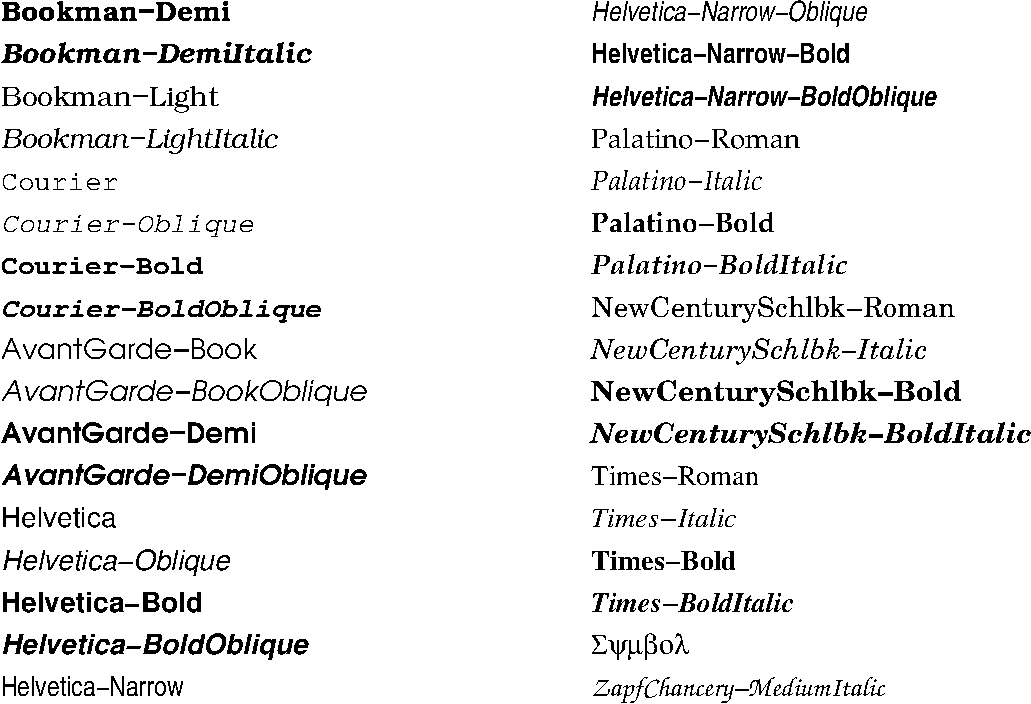
\includegraphics[width=0.95\linewidth]{fonts.pdf}

% -----

% \noteseparator

% -----

\section{MIDI Instruments}
\label{sec:midiinstr}

\subsection{Standard instruments}

The following is a complete list of the General MIDI standard instruments,
subdivided according to instrument family. Remember, when using \abcmid{}
the instrument number must be decreased by 1.

\bigskip

% -----
\newcommand{\mi}[2]
{\textbf{#1}. #2}
% -----

{\small
{\centering
\begin{supertabular}{p{0.3\linewidth}p{0.3\linewidth}p{0.3\linewidth}}
  %
  \textbf{Piano} & \textbf{Chromatic Percussion} &
  \textbf{Organ} \\
  %
  \mi{1}{Acoustic Grand} & \mi{9}{Celesta} & \mi{17}{Drawbar Organ} \\
  \mi{2}{Bright Acoustic} & \mi{10}{Glockenspiel} & \mi{18}{Percussive Organ} \\
  \mi{3}{Electric Grand} & \mi{11}{Music Box} & \mi{19}{Rock Organ} \\
  \mi{4}{Honky-Tonk} & \mi{12}{Vibraphone} & \mi{20}{Church Organ} \\
  \mi{5}{Electric Piano 1} & \mi{13}{Marimba} & \mi{21}{Reed Organ} \\
  \mi{6}{Electric Piano 2} & \mi{14}{Xylophone} & \mi{22}{Accordion} \\
  \mi{7}{Harpsichord} & \mi{15}{Tubular Bells} & \mi{23}{Harmonica} \\
  \mi{8}{Clavinet} & \mi{16}{Dulcimer} & \mi{24}{Tango Accordion} \\
  %
  \rule{0pt}{0.5cm} \textbf{Guitar} & \textbf{Bass} &
  \textbf{Solo Strings} \\
  \mi{25}{Nylon String Guitar} & \mi{33}{Acoustic Bass} & \mi{41}{Violin} \\
  \mi{26}{Steel String Guitar} & \mi{34}{Electric Bass(finger)} &
  \mi{42}{Viola} \\
  \mi{27}{Electric Jazz Guitar} & \mi{35}{Electric Bass(pick)} &
  \mi{43}{Cello} \\
  \mi{28}{Electric Clean Guitar} & \mi{36}{Fretless Bass} &
  \mi{44}{Contrabass} \\
  \mi{29}{Electric Muted Guitar} & \mi{37}{Slap Bass 1} & \mi{45}{Tremolo Strings} \\
  \mi{30}{Overdriven Guitar} & \mi{38}{Slap Bass 2} & \mi{46}{Pizzicato Strings} \\
  \mi{31}{Distortion Guitar} & \mi{39}{Synth Bass 1} & \mi{47}{Orchestral Strings} \\
  \mi{32}{Guitar Harmonics} & \mi{40}{Synth Bass 2} & \mi{48}{Timpani} \\
  %
  \rule{0pt}{0.5cm} \textbf{Ensemble} & \textbf{Brass} & \textbf{Reed} \\
  %
  \mi{49}{String Ensemble 1} & \mi{57}{Trumpet} & \mi{65}{Soprano Sax} \\
  \mi{50}{String Ensemble 2} & \mi{58}{Trombone} & \mi{66}{Alto Sax} \\
  \mi{51}{SynthStrings 1} & \mi{59}{Tuba} & \mi{67}{Tenor Sax} \\
  \mi{52}{SynthStrings 2} & \mi{60}{Muted Trumpet} & \mi{68}{Baritone Sax} \\
  \mi{53}{Choir Aahs} & \mi{61}{French Horn} & \mi{69}{Oboe} \\
  \mi{54}{Voice Oohs} & \mi{62}{Brass Section} & \mi{70}{English Horn} \\
  \mi{55}{Synth Voice} & \mi{63}{SynthBrass 1} & \mi{71}{Bassoon} \\
  \mi{56}{Orchestra Hit} & \mi{64}{SynthBrass 2} &\mi{72}{Clarinet} \\
  %
  \rule{0pt}{0.5cm} \textbf{Pipe} & \textbf{Synth Lead} & \textbf{Synth Pad} \\
  %
  \mi{73}{Piccolo} & \mi{81}{Lead 1 (square)} & \mi{89}{Pad 1 (new age)} \\
  \mi{74}{Flute} & \mi{82}{Lead 2 (sawtooth)} & \mi{90}{Pad 2 (warm)} \\
  \mi{75}{Recorder} & \mi{83}{Lead 3 (calliope)} & \mi{91}{Pad 3 (polysynth)} \\
  \mi{76}{Pan Flute} & \mi{84}{Lead 4 (chiff)} & \mi{92}{Pad 4 (choir)} \\
  \mi{77}{Blown Bottle} & \mi{85}{Lead 5 (charang)} & \mi{93}{Pad 5 (bowed)} \\
  \mi{78}{Skakuhachi} & \mi{86}{Lead 6 (voice)} & \mi{94}{Pad 6 (metallic)} \\
  \mi{79}{Whistle} & \mi{87}{Lead 7 (fifths)} & \mi{95}{Pad 7 (halo)} \\
  \mi{80}{Ocarina} & \mi{88}{Lead 8 (bass+lead)} & \mi{96}{Pad 8 (sweep)} \\
  %
  \rule{0pt}{0.5cm} \textbf{Synth Effects} & \textbf{Ethnic} & \textbf{Percussive} \\
  %
  \mi{97}{FX 1 (rain)} & \mi{105}{Sitar} & \mi{113}{Tinkle Bell} \\
  \mi{98}{FX 2 (soundtrack)} & \mi{106}{Banjo} & \mi{114}{Agogo} \\
  \mi{99}{FX 3 (crystal)} & \mi{107}{Shamisen} & \mi{115}{Steel Drums} \\
  \mi{100}{FX 4 (atmosphere)} & \mi{108}{Koto} & \mi{116}{Woodblock} \\
  \mi{101}{FX 5 (brightness)} & \mi{109}{Kalimba} & \mi{117}{Taiko Drum} \\
  \mi{102}{FX 6 (goblins)} & \mi{110}{Bagpipe} & \mi{118}{Melodic Tom} \\
  \mi{103}{FX 7 (echoes)} & \mi{111}{Fiddle} & \mi{119}{Synth Drum} \\
  \mi{104}{FX 8 (sci-fi)} & \mi{112}{Shanai} & \mi{120}{Reverse Cymbal} \\
  %
  \rule{0pt}{0.5cm} \textbf{Sounds Effects} & & \\
  %
  \mi{121}{Guitar Fret Noise} & & \\
  \mi{122}{Breath Noise} & & \\
  \mi{123}{Seashore} & & \\
  \mi{124}{Bird Tweet} & & \\
  \mi{125}{Telephone Ring} & & \\
  \mi{126}{Helicopter} & & \\
  \mi{127}{Applause} & & \\
  \mi{128}{Gunshot} & & \\
\end{supertabular}
} % \centering
} % \small

% -----
\newcommand{\miwn}[3]
{\textbf{#1}. \car{#2} #3}
% -----

\subsection{Percussion Instruments}
\label{sec:perc}

These instruments can be used with \metacmd{MIDI drum}, or using the
corresponding note in the MIDI channel 10.

\medskip

{\small
{\centering
\begin{tabular}{p{0.3\linewidth}p{0.3\linewidth}p{0.3\linewidth}}
  %
  \miwn{35}{B,,,}{Acoustic Bass Drum} & \miwn{36}{C,,~}{Bass Drum 1} &
  \miwn{37}{\char94C,,}{Side Stick} \\
  \miwn{38}{D,,~}{Acoustic Snare} &
  \miwn{39}{\char94D,,}{Hand Clap} &
  \miwn{40}{E,,~}{Electric Snare} \\
  \miwn{41}{F,,~}{Low Floor Tom} &
  \miwn{42}{\char94F,,}{Closed Hi Hat} &
  \miwn{43}{G,,~}{High Floor Tom} \\
  \miwn{44}{\char94G,,}{Pedal Hi-Hat} & \miwn{45}{A,,~}{Low Tom} &
  \miwn{46}{\char94A,,}{Open Hi-Hat} \\
  \miwn{47}{B,,~}{Low-Mid Tom} & \miwn{48}{C,~~}{Hi Mid Tom} &
  \miwn{49}{\char94C,~}{Crash Cymbal 1} \\
  \miwn{50}{D,~~}{High Tom} & \miwn{51}{\char94D,~}{Ride Cymbal 1} &
  \miwn{52}{E,~~}{Chinese Cymbal} \\
  \miwn{53}{F,~~}{Ride Bell} & \miwn{54}{\char94F,~}{Tambourine} &
  \miwn{55}{G,~~}{Splash Cymbal} \\
  \miwn{56}{\char94G,~}{Cowbell} & \miwn{57}{A,~~}{Crash Cymbal 2} &
  \miwn{58}{\char94A,~}{Vibraslap} \\
  \miwn{59}{B,~~}{Ride Cymbal 2} & \miwn{60}{C~~~}{Hi Bongo} &
  \miwn{61}{\char94C~~}{Low Bongo} \\
  \miwn{62}{D~~~}{Mute Hi Conga} &
  \miwn{63}{\char94D~~}{Open Hi Conga} &
  \miwn{64}{E~~~}{Low Conga} \\
  \miwn{65}{F~~~}{High Timbale} & \miwn{66}{\char94F~~}{Low Timbale} &
  \miwn{67}{G~~~}{High Agogo} \\
  \miwn{68}{\char94G~~}{Low Agogo} & \miwn{69}{A~~~}{Cabasa} &
  \miwn{70}{\char94A~~}{Maracas} \\
  \miwn{71}{B~~~}{Short Whistle} & \miwn{72}{c~~~}{Long Whistle} &
  \miwn{73}{\char94c~~}{Short Guiro} \\
  \miwn{74}{d~~~}{Long Guiro} & \miwn{75}{\char94d~~}{Claves} &
  \miwn{76}{e~~~}{Hi Wood Block} \\
  \miwn{77}{f~~~}{Low Wood Block} & \miwn{78}{\char94f~~}{Mute Cuica} &
  \miwn{79}{g~~~}{Open Cuica} \\
  \miwn{80}{\char94g~~}{Mute Triangle} &
  \miwn{81}{a~~~}{Open Triangle} & \\
\end{tabular}}}

% \noteseparator

\end{document}

% ----- End of file abcplus_en.tex
